% Initial version by Darian Muresan, Ph.D.
% Edit and adjust as needed.

\documentclass[12pt]{cornell}

% add index support
\makeindex

% graphing programs
\usepackage{color}
\usepackage{psfrag}
\usepackage{verbatim}
\usepackage{fancyhdr}
%\usepackage{titlesec}
\usepackage{fancyvrb} 
% hyperlink programs
\usepackage[pdfmark, 
breaklinks=true, 
colorlinks=true,
citecolor=blue,
linkcolor=blue,
menucolor=black,
pagecolor=black,
urlcolor=blue
]{hyperref} % links in pdf
%\usepackage[colorlinks]{hyperref} % links in dvi
\usepackage{listings}
\usepackage{amsfonts} 
\usepackage{amssymb} 
%\usepackage{tabto}

\usepackage{tabularx,colortbl}
\usepackage[chapter]{algorithm} 
\usepackage{algorithmic} 
\usepackage{blindtext}
\usepackage{imakeidx}


\definecolor{DarkGreen}{rgb}{0,0.6,0}
\definecolor{mygreen}{rgb}{0,0.6,0}
\definecolor{mygray}{rgb}{0.5,0.5,0.5}
\definecolor{mymauve}{rgb}{0.58,0,0.82}

\usepackage{tocloft}
\usepackage{amsmath}
\usepackage{tcolorbox}
\usepackage{enumitem}
\usepackage{longtable}
%\usepackage{textcomp}
\usepackage{txfonts}

%part for \part titles
%chap for \chapter titles
%sec for \section titles
%subsec for \subsection titles
%subsubsec for \subsubsection titles
%para for \paragraph titles
%subpara for \subparagraph titles
%fig for figure \caption titles
%subfig for subfigure \caption titles
%tab for table \caption titles
%subtab for subtable \caption titles

% update chapter number spacing
\setlength{\cftchapnumwidth}{2em}
\setlength{\cftsecnumwidth}{2.5em}
\setlength{\cftsubsecnumwidth}{3.5em}
\setlength{\cftsubsubsecnumwidth}{4.5em}

\addtolength{\cftsecindent}{0.5em}
\addtolength{\cftsubsecindent}{0.5em}
\addtolength{\cftsubsubsecindent}{0.5em}

%\titlespacing*{\chapter}{0pt}{-50pt}{20pt}
%\titleformat{\chapter}[display]{\normalfont\huge\bfseries}{\chaptertitlename\ 
%\thechapter}{20pt}{\Huge}
%\pagestyle{fancy}
%\pagestyle{cornell}
%
%\rhead{F054-021-0172}
%\chead{Nonlinear Enhancement of Visual Target Detection (AF05-T021)}
%\lhead{GSTI}
%\lfoot{\scriptsize Use or disclosure of data on this page is subject
%to the restriction on the title page of this proposal.}
%\cfoot{}
%\rfoot{\thepage}

\newfont{\Bp}{msbm10}
\newfont{\BpBig}{msbm10 scaled\magstep2}
\newfont{\Sc}{eusm10}
\newfont{\ScBig}{eusm10 scaled\magstep3}
\newfont{\Fr}{eufm10}
\newfont{\FrBig}{eufm10 scaled\magstep1}

% some commands:
\newcommand{\dxi}{{\tt m\_xDeltaInput}}
\newcommand{\dyi}{{\tt m\_yDeltaInput}}
\newcommand{\dci}{{\tt m\_cDeltaInput}}
\newcommand{\dxo}{{\tt m\_xDeltaOutput}}
\newcommand{\dyo}{{\tt m\_yDeltaOutput}}
\newcommand{\dco}{{\tt m\_cDeltaOutput}}
\newcommand{\ttf}[1]{{\tt #1}}
\newcommand{\tbl}[2]{{\begin{tabular}{c} #1 \\ #2 \end{tabular}}}

\newcommand{\urltwo}[2]{\mbox{\href{#1}{\tt #2}}}
\newcommand{\qnorm}[1]{\|#1\|_{\bQ}}
\newcommand{\qdot}[2]{\lrb #1, #2 \rrb_{\bQ}}
\newcommand{\kdot}[2]{\lrb #1, #2 \rrb_{\bf k}}
\newcommand{\tdot}[2]{\lrb #1, #2 \rrb}
\newcommand{\mydiff}[2]{\lrb #1 - #2 \rrb}
\newcommand{\lena}{\textit{lena}}
\newcommand{\barb}{\textit{barbara}}
\newcommand{\boat}{\textit{boat}}
\newcommand{\leaves}{\textit{leaves}}
\newcommand{\rings}{\textit{rings}}
\newcommand{\treg}{\textit{train region}}
\newcommand{\dreg}{\textit{denoise region}}
\newcommand{\oreg}{\textit{overlap region}}
\newcommand{\sil}{\sigma_l^2}
\newcommand{\sn}{\sigma^2}
\newcommand{\bn}{{\mbox{\bf \FrBig N}}}
\newcommand{\n}{\mbox{\Fr N}}
%\newcommand{\bn}{\bf N}
%\newcommand{\n}{N}
\newcommand{\bY}{\textbf{Y}}
\newcommand{\bX}{\textbf{X}}
\newcommand{\bb}{\textbf{b}}
\newcommand{\bu}{\textbf{u}}
\newcommand{\bv}{\textbf{v}}
\newcommand{\by}{\textbf{y}}
\newcommand{\bx}{\textbf{x}}
\newcommand{\be}{\textbf{e}}
\newcommand{\bz}{\textbf{z}}
\newcommand{\bs}{\textbf{s}}
\newcommand{\bw}{\textbf{w}}
\newcommand{\bQ}{\textbf{Q}}
\newcommand{\bphi}{\textbf{$\phi$}}
\newcommand{\lsb}{\left[}
\newcommand{\rsb}{\right]}
\newcommand{\lrb}{\left(}
\newcommand{\rrb}{\right)}
\newcommand{\lcb}{\left\{}
\newcommand{\rcb}{\right\}}
\newcommand{\R}{\mbox{\BpBig R}}
\newcommand{\F}{{\cal F}}
\newcommand{\Fk}{\mbox{\Sc F}}
\newcommand{\bQF}{\textbf{Q}_{\mbox{\Sc F}}}
\newcommand{\N}{{\cal N}}
\newcommand{\xlz}{X_l(z)}
\newcommand{\xhz}{X_h(z)}
\newcommand{\xz}{X(z)}
\newcommand{\pr}{ perfect reconstruction }
\newcommand{\smb}{Smith-Barnwell }
\newcommand{\xw}{X(e^{j\omega})}
\newcommand{\xmw}{X(-e^{j\omega})}
\newcommand{\dw}{D(e^{j\omega})}
\newcommand{\dmw}{D(-e^{j\omega})}
\newcommand{\ew}{E(e^{j\omega})}
\newcommand{\emw}{E(-e^{j\omega})}
\newcommand{\fw}{F_0(e^{j\omega})}
\newcommand{\fmw}{F_0(-e^{j\omega})}
\newcommand{\hoz}{H_1(z)}
\newcommand{\hzz}{H_0(z)}
\newcommand{\goz}{G_1(z)}
\newcommand{\gzz}{G_0(z)}
\newcommand{\hzw}{H_{0}(e^{j\omega})}
\newcommand{\hzmw}{H_{0}(-e^{j\omega})}
\newcommand{\hzcw}{H_{0}(e^{-j\omega})}
\newcommand{\how}{H_1(e^{j\omega})}
\newcommand{\homw}{H_1(-e^{j\omega})}
\newcommand{\gzw}{G_0(e^{j\omega})}
\newcommand{\gzmw}{G_0(-e^{j\omega})}
\newcommand{\gow}{G_1(e^{j\omega})}
\newcommand{\gomw}{G_1(-e^{j\omega})}
\newcommand{\wl}{e^{-jwL}}
\newcommand{\aqua}{\textit{AQua with OR }}
\newtheorem{theorem}{Theorem}
\newtheorem{lemma}{Lemma}
\newtheorem{corollary}{Corollary}
\newtheorem{claim}{Claim}
\newtheorem{definition}{Definition}
\newenvironment{proof}{\noindent{\em Proof.}}{\ \hfill Q.E.D.}
%\newtheorem{moduleCount}{L}
\newcommand*{\labelfile}[1]{%
  \label{file:#1}%
}

\lstset{ %
  backgroundcolor=\color{white},   % choose the background color; you must add \usepackage{color} or \usepackage{xcolor}
  basicstyle=\footnotesize,        % the size of the fonts that are used for the code
  breakatwhitespace=false,         % sets if automatic breaks should only happen at whitespace
  breaklines=true,                 % sets automatic line breaking
  captionpos=b,                    % sets the caption-position to bottom
  commentstyle=\color{DarkGreen},    % comment style
  deletekeywords={...},            % if you want to delete keywords from the given language
  escapeinside={\%*}{*)},          % if you want to add LaTeX within your code
  extendedchars=true,              % lets you use non-ASCII characters; for 8-bits encodings only, does not work with UTF-8
  %frame=single,                   % adds a frame around the code
  keepspaces=true,                 % keeps spaces in text, useful for keeping indentation of code (possibly needs columns=flexible)
  keywordstyle=\color{blue},       % keyword style
  language=C++,                    % the language of the code
  morekeywords={*,...},            % if you want to add more keywords to the set
  numbers=left,                    % where to put the line-numbers; possible values are (none, left, right)
  numbersep=5pt,                   % how far the line-numbers are from the code
  numberstyle=\tiny\color{mygray}, % the style that is used for the line-numbers
  rulecolor=\color{black},         % if not set, the frame-color may be changed on line-breaks within not-black text (e.g. comments (green here))
  showspaces=false,                % show spaces everywhere adding particular underscores; it overrides 'showstringspaces'
  showstringspaces=false,          % underline spaces within strings only
  showtabs=false,                  % show tabs within strings adding particular underscores
  stepnumber=1,                    % the step between two line-numbers. If it's 1, each line will be numbered
  stringstyle=\color{mymauve}     % string literal style
  %tabsize=2,                      % sets default tabsize to 2 spaces
  %caption=\lstname                % show the filename of files included with \lstinputlisting; also try caption instead of title
}

% Uncomment draftcopy to get the word DRAFT boldly across the first page
%   By the way, xdvi won't show it but it will come out when you print
%\usepackage[light,all]{draftcopy}		% DRAFT on first page
%\draftcopySetGrey{.97}
%\draftcopyName{Confidential}{150}
%\draftcopFirstPage{1}

% Uncomment drafthead to get the date and DRAFT in the header of pages
% that are normallly numbered on the top, pages 2-n of each chapter for example
% This doesn't work with centered page numbers: \pagestyle{cornellc}
%\usepackage{drafthead}

% Including selective chapters:
% use this to selectively process chapters, etc.  Put a % in front of
% the sections that you don't want done this time.  Includes are
% used instead of \input so that LaTeX will keep track of chapters and
% pages without processing everything.  Don't let any spaces creep in
% around the words or it will not work!


\includeonly{
prologue,
manIntroduction,
Identifyprojecttitle,
Referenceddocuments,
Currentsystemorsituation,
Justificationforandnatureofchanges,
Conceptsfortheproposedsystem,
Operationalscenarios,
Summaryofimpacts,
Analysisoftheproposedsystem,
Notes

}

\makeindex

\begin{document}

\pagenumbering{roman}
\singlespacing
% File: prologue.tex
% Thesis prologue:  Title page, acknowledgements, table of contents,
% list of figures, and list of tables.
%
% this file is to be \include'd after the \begin{document}

% Cornell-style title page
\begin{titlepage}
        \title{Projects Assignments}
        \author{Ashay Pable\\Divyamshu Mandadi\\Neel Savani\\ Stevens.edu }
        \conferraldate{}{\today} \maketitle
\end{titlepage}

% Copyright page
%\begin{copyrightpage}
\makecopyright
%\end{copyrightpage}

% Abstract: the abstract body is pulled from the file abstract.tex;
%  the title is pulled from the \title command in the titlepage section
\begin{abstract}
        %\makeabstitle
        \input abstract      % puts the abstract file here
\end{abstract}

% Biographical information pulled from file bio.tex
%\begin{biosketch} \input bio \end{biosketch}

% Dedication (optional):  pulls information from file dedication.tex
%\begin{dedication} 
%\input dedicate 
%\end{dedication}

% Acknowledgements:  pulls information from file acknow
%\begin{acknowledgements} \input acknow \end{acknowledgements}

% Table of contents
\contentspage

% If you have no tables or figures put a % in front of the list page line
% List of tables
\tablelistpage

% List of figures
\figurelistpage



\setcounter{page}{1}        % set page counter
\pagenumbering{arabic}      % set page number style
\pagestyle{fancy}         % top right page numbers
%\pagestyle{cornell}
%\pagestyle{cornellc}       % centered page numbers, disables drafthead

\renewcommand{\chaptermark}[1]{\markboth{#1}{}}
\renewcommand{\sectionmark}[1]{\markright{#1}{}}

\fancyhead{} % clear all fields

\lhead{Chapter \thechapter}
%\lhead{\thechapter}
\chead{\leftmark}
\rhead{\thepage}


\lfoot{Chapter \thechapter}
\cfoot{\copyright Stevens -- \today \mbox{} -- Project Name}
\rfoot{\thepage}

\renewcommand{\headrulewidth}{0.4pt}
\renewcommand{\footrulewidth}{0.4pt}

%\rhead{F054-021-0172}
%\chead{Nonlinear Enhancement of Visual Target Detection (AF05-T021)}
%\lhead{GSTI}
%\lfoot{\scriptsize Use or disclosure of data on this page is subject
%to the restriction on the title page of this proposal.}
%\cfoot{}
%\rfoot{\thepage}


\singlespacing
% \chapter{Introduction \\
% \small{\textit{-- Author Name}} 
% % \index{Chapter!introduction}
% \index{introduction}
% \label{Chapter::Introduction}}

% \chapter{Analysis of the proposed system \\ 
% % \small{\textit{-- Author Name}}
% \index{Analysis of the proposed system}
% \label{Chapter::Analysisoftheproposedsystem}}

% % Add a section and label it so that we can reference it later
% \section{My Section \label{Section::MySection}}


% % add a new page
% \newpage

% Hi there world!  Here is an example of a note\footnote{Here is a reference 
% to Figure \ref{Figure::manAgile} and an indexed keyword\index{keyword}.}

\chapter{Identify project and Mission statement \\
% \small{\textit{-- Ashay Pable}} 
%\index{Chapter!Homework One -- Requirements}
\index{Identify project and Mission statement}
\label{Chapter::Identify project and Mission statement}}

% Add a section and label it so that we can reference it later
\section{Team Members \label{Section::teamMembers}}
\begin{enumerate}
  \item \textbf{Ashay Pable} : I am a Masters in Software Engineering student. I have worked as a software
developer for 4 years in India with a wide range of experience from Artificial Intelligence to
3D Graphics development. I have a keen interest in automation powered by AI and research
in contributing fields. My experience as a developer has made me realise the importance of
planning and documentation before initiation of a project
  \item \textbf{Divyamshu Mandadi} : My name is Divyamshu Mandadi and I’m currently in my third
semester doing my Masters in Software Engineering. Before moving to the US I have
worked as a Software Developer in India. My experience while working there combined
with the curiosity to learn more about the Software development processes led me here.
  \item \textbf{Neel Savani} : My name is Neel Savani. I had completed my under-graduation in Informa-
tion and Technology at birla vishwakarma mahavidhyalaya. I am currently in my second-
semester pursuing my masters in Software engineering. I am interested in developing soft-
ware.
\end{enumerate}

\section{Team Name \label{Section::teamName}}
"Group 3 - Inventory Management System for Retail Stores"
\section{Project Chosen \label{Section::projectChosen}}
\begin{itemize}
 \item Inventory Management system for Retail Stores.
 \item The project's goal is to create an intuitive and efficient inventory management system that will provide a retail business with real-time visibility into inventory levels and movement.
\end{itemize}
\section{Project Mission Statement \label{Section::projectMissionStatement}}
Our mission is to provide seamless and continuous supply of inventory so that customers needs are catered to in an efficient manner. Our system will provide an intuitive user interface that enables efficient recording and management of each item in the inventory. Retailers will be able to minimize stockouts, manage inventory levels for maximum profitability, and base data-driven choices on real-time inventory levels. This system provides a comprehensive solution that improves inventory management for retail establishments, frees up time, reduces expenses, and increases overall operational performance.

% \cite{GM1998}.

%\begin{figure}
%\centering
%\scalebox{0.8}{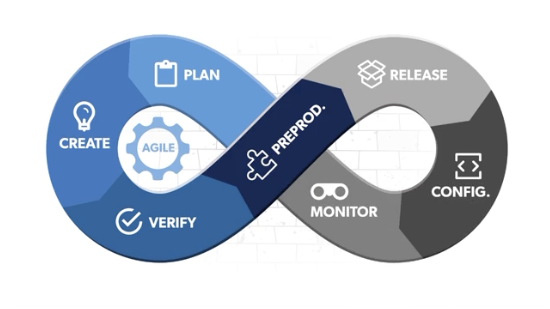
\includegraphics{Figures/manAgileProcess.png}}
%\caption{\label{Figure::manAgile} Figure of the continuous agile process.}
%\end{figure}

% add a new page
\newpage

\chapter{Referenced documents \\ 
% \small{\textit{-- Author Name}}
\index{Referenced documents}
\label{Chapter::Referenceddocuments}} 

Several recent studies, relevant research papers and articles with keywords such as “Inventory Management” and “Retail” or “Retail Sector” and “Operations Research” Databases such as Google Scholar, Science Direct and Z-library were also used. We also used Oracle Retail Store Inventory Management Documentation Library extensively to identify their features, limitations and how through our system we can mitigate them.\cite{ORACLE}

\newpage
\chapter{Current system or situation \\ 
% \small{\textit{-- Author Name}}
\index{Current system or situation}
\label{Chapter::Currentsystemorsituation}} 
\section{Background, objectives, and scope \label{Section::Backgroundobjectivesandscope}}
The instore inventory management system is an essential tool for managing inventory in a retail store. The system is responsible for tracking the movement of goods, monitoring stock levels, and ensuring that the right products are available at the right time. The current manual inventory management system is time-consuming, prone to errors, and lacks real-time visibility of inventory levels. The new instore inventory management system aims to address these challenges by automating the process, providing accurate and real-time inventory information, and enabling efficient and effective management of inventory levels.
The primary objective of the instore inventory management system is to improve the accuracy, efficiency, and effectiveness of inventory management in the retail store. Specifically, the system aims to achieve the following objectives:
\begin{enumerate}    
\item Real-time inventory visibility: Provide accurate and real-time visibility of inventory levels to store managers and staff.

\item Automated inventory tracking: Automate the process of tracking inventory movement, including receiving, stocking, and selling products.

\item Efficient inventory management: Enable efficient management of inventory levels, including setting reorder points, managing stock levels, and reducing waste.

\item Improved decision-making: Provide data analytics and reporting tools to support informed decision-making related to inventory management.
\end{enumerate}
The instore inventory management system will be designed to manage inventory for a single retail store. The system will be integrated with the existing point-of-sale (POS) system to provide real-time inventory information. The system will track the movement of goods from the time they are received into the store until they are sold or removed from inventory. The system will include features for setting reorder points, generating purchase orders, and monitoring stock levels. The system will also include reporting and data analytics tools to support informed decision-making related to inventory management.

The system will be designed to be user-friendly and intuitive to use, with minimal training required for store managers and staff. The system will be scalable, allowing for the addition of new products and the expansion of the store. The system will be designed to be compatible with existing hardware and software systems in the store. Finally, the system will be secure and reliable, ensuring the confidentiality and integrity of inventory data.

\section{Operational policies and constraints \label{Section::Operationalpoliciesandconstraints}}

\textbf{Operational policies:}
\begin{enumerate}
\item Access control: Access to the instore inventory management system will be restricted to authorized personnel only. Access credentials will be assigned on a need-to-know basis.
\item Data protection: The system will store inventory data in a secure and encrypted manner. Data backups will be taken regularly to ensure data integrity and availability in case of system failure.
\item Maintenance and support: The system will be maintained and supported by trained personnel to ensure optimal performance and reliability. Maintenance schedules will be developed to minimize disruptions to store operations.
\item Training and documentation: Store managers and staff will be provided with adequate training and documentation to ensure proper use of the system. Training will be ongoing, and documentation will be updated as needed.
\item Change management: Changes to the system, including upgrades and modifications, will be managed through a formal change management process. Changes will be tested and validated before implementation.

\end{enumerate}

\noindent
\textbf{Constraints:}
\begin{enumerate}
\item Budget: The implementation of the instore inventory management system will be subject to budgetary constraints. The cost of hardware, software, and personnel will need to be within the allocated budget.

\item Integration with existing systems: The system will need to be integrated with the existing point-of-sale (POS) system, which may have limitations on compatibility.

\item Technical limitations: The system will be subject to technical limitations, such as hardware capacity and bandwidth limitations.

\item User adoption: The success of the system will depend on the adoption by store managers and staff. The system will need to be user-friendly and intuitive to ensure adoption.

\item Regulatory compliance: The system will need to comply with all relevant regulatory requirements, including data privacy and security regulations.
\end{enumerate}

\section{Description of the current system or situation \label{Section::Descriptionofthecurrentsystemorsituation}}
The current inventory management system in the retail store is a manual process that is time-consuming and prone to errors. The process involves tracking inventory movement, monitoring stock levels, and placing orders for replenishment. The system relies on physical counts, spreadsheets, and manual record-keeping to track inventory.

The process begins with the receipt of goods from suppliers. The store manager or staff checks the goods against the purchase order and records the receipt in a manual log. The goods are then moved to the storage area, and the stock level is updated manually.

When items are sold, the store manager or staff records the sale in the point-of-sale (POS) system and manually updates the inventory count. When stock levels fall below a certain threshold, the store manager or staff manually creates a purchase order to replenish the inventory.

The current system has several limitations. Firstly, the manual process is time-consuming and prone to errors, leading to inaccurate inventory counts and stockouts. Secondly, the system lacks real-time visibility of inventory levels, making it challenging to manage stock levels effectively. Finally, the manual process does not provide data analytics and reporting tools to support informed decision-making related to inventory management.\cite{OR2020}
\begin{figure}[H]
  \centering
   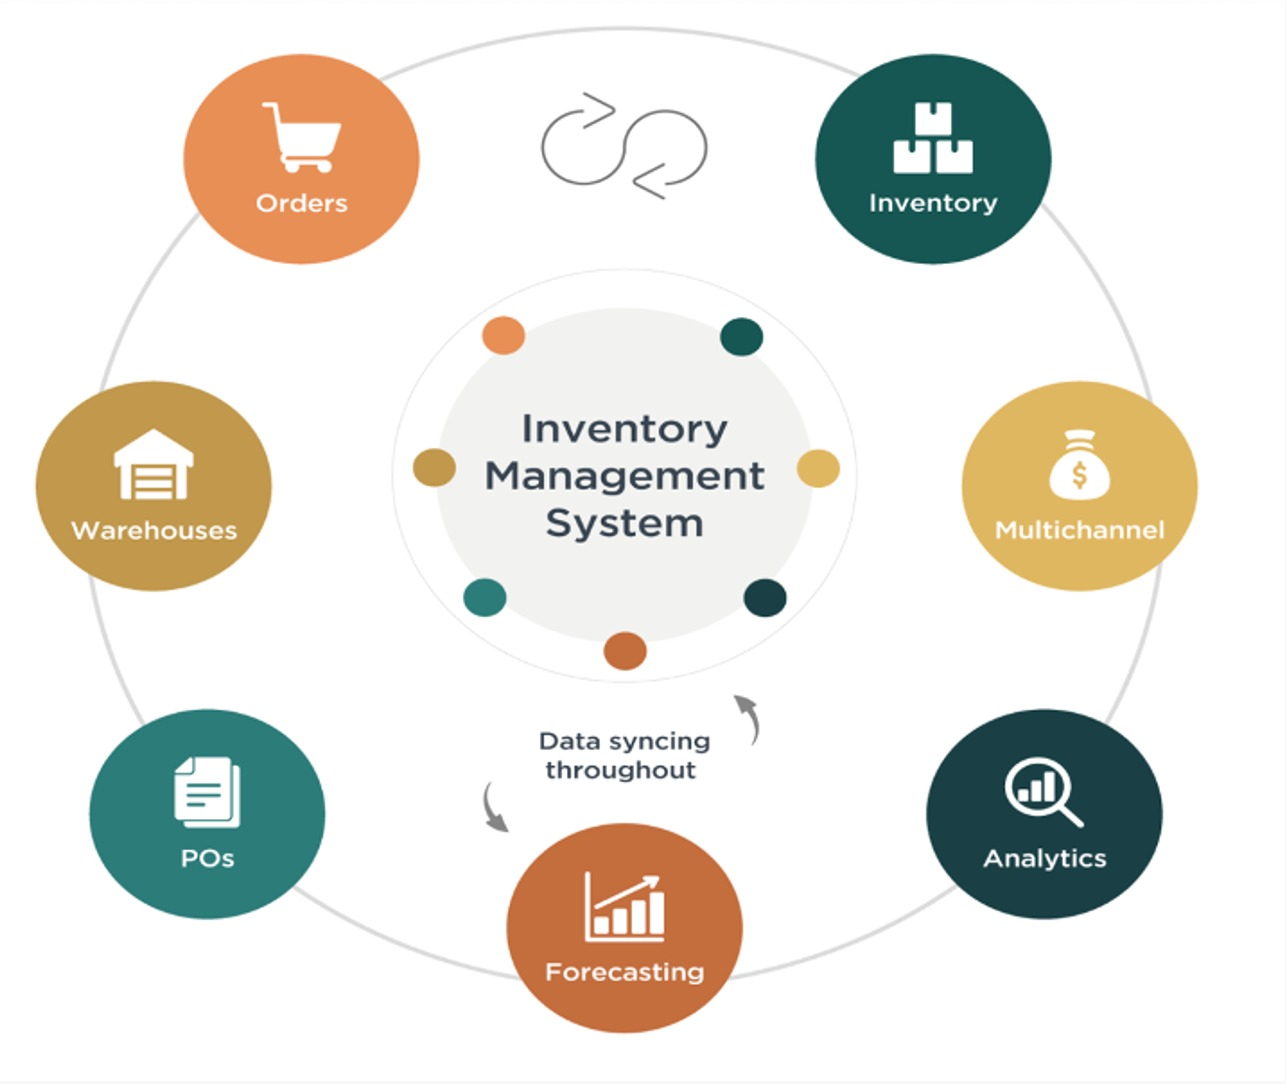
\includegraphics[width=9cm]{Figures/SpiritDiagram.jpeg}
  \caption{Overview Diagram}
\label{}
\end{figure}
\section{Modes of operation for the current system or situation \label{Section::Modesofoperationforthecurrentsystemorsituation}}
The current inventory management system in the retail store operates in the following modes:

\begin{enumerate}
    
\item Receiving mode: This mode is activated when goods are received from suppliers. The store manager or staff checks the goods against the purchase order and records the receipt in a manual log. The goods are then moved to the storage area, and the stock level is updated manually.

\item Stocking mode: This mode is activated when goods are moved from the storage area to the shelves or display areas. The store manager or staff manually updates the inventory count.

\item Selling mode: This mode is activated when items are sold to customers. The store manager or staff records the sale in the point-of-sale (POS) system and manually updates the inventory count.

\item Ordering mode: This mode is activated when stock levels fall below a certain threshold. The store manager or staff manually creates a purchase order to replenish the inventory.

\end{enumerate}

The current system operates in a sequential manner, with each mode depending on the previous mode's completion. The system lacks real-time visibility of inventory levels and does not provide automated inventory tracking or reporting tools.

\section{User classes and other involved personnel \label{Section::Userclassesandotherinvolvedpersonnel}}
The following are the user classes and other personnel involved in the instore inventory management system:

\begin{enumerate}

    \item Store manager: The store manager is responsible for managing the inventory and overseeing the instore inventory management system's operation. The store manager is responsible for setting up the system, assigning access credentials to authorized personnel, and ensuring the system's proper use.


    \item Store staff: The store staff is responsible for handling the goods, updating inventory levels, and generating reports using the instore inventory management system. The store staff will be provided with adequate training and documentation to ensure proper use of the system.

    \item IT personnel: The IT personnel will be responsible for    installing, configuring, and maintaining the hardware and software components of the system. They will also be responsible for ensuring the system's security, integrity, and availability.

    \item Suppliers: The suppliers will be involved in the system through the receipt of purchase orders generated by the system. The suppliers will need to ensure timely delivery of goods and accurate order fulfillment.

    \item Customers: The customers indirectly interact with the system by purchasing goods that are managed by the instore inventory management system. The system will ensure that the customers have access to the products they need when they need them, improving their shopping experience.
    
\end{enumerate}

The involvement of these user classes and personnel is critical to the success of the instore inventory management system, and their cooperation and support will be essential for the system's effective implementation and operation.

\section{Support environment \label{Section::Supportenvironment}}
\begin{enumerate}
    \item Help desk: A help desk will be set up to provide support and assistance to store managers and staff using the system. The help desk will be staffed by trained personnel who can provide technical assistance and troubleshooting support.

    \item Online documentation: The instore inventory management system will include online documentation that provides detailed instructions on how to use the system's features and functionality. The documentation will be regularly updated and available online for easy access.

    \item Training sessions: Store managers and staff will be provided with adequate training on the system's operation and functionality. Training sessions will be conducted both online and in-person and will be tailored to the specific needs of the user class.

    \item Maintenance and support team: A dedicated maintenance and support team will be responsible for ensuring the system's optimal performance and reliability. The team will be available to respond to system issues and perform maintenance tasks as required.

    \item Vendor support: The system vendor will provide technical support and assistance in case of system issues or malfunctions. The vendor will be responsible for ensuring that the system operates as intended and meets the user's requirements.
    
\end{enumerate}


\newpage
\chapter{Justification for and nature of changes \\ 
% \small{\textit{-- Author Name}}
\index{Justification for and nature of changes}
\label{Chapter::Justificationforandnatureofchanges}} 
\section{Justication of changes \label{Section::Justicationofchanges}}
The justification for these changes is to address several key issues identified through a recent analysis of our company's operations. This analysis revealed a number of inefficiencies and bottlenecks that have been negatively impacting productivity and profitability. The proposed changes aim to streamline workflows, improve communication and collaboration, and optimize resource allocation to achieve better results.

\noindent
There are several reasons why changes are required, including:

\begin{enumerate}

    \item New business requirements: The business requirements for the instore inventory management system may change as the business grows or as market conditions change. These changes may require modifications to the system to support new requirements.

    \item Technological advancements: Advancements in technology may provide new opportunities to improve the system's performance, reliability, and scalability. These advancements may require changes to the system to take advantage of the new capabilities.

    \item User feedback: Feedback from users may reveal areas where the system could be improved to better meet their needs. This feedback may prompt changes to the system's design or functionality.

    \item Regulatory requirements: Changes in regulatory requirements may require modifications to the system to ensure compliance with new regulations.

    \item External factors: External factors, such as changes in the competitive landscape or economic conditions, may require modifications to the system to remain competitive or to reduce costs.

\end{enumerate}

The nature of changes in the instore inventory management system can range from minor modifications to major overhauls. Changes may involve adding new functionality, modifying existing functionality, or removing functionality that is no longer required. Changes may also involve modifications to the system's architecture or infrastructure to improve performance, reliability, or scalability.


\section{Description of desired changes \label{Section::Descriptionofdesiredchanges}}
The instore inventory management system requires several changes to enhance its performance, reliability, and scalability. Some of the desired changes are:

\begin{enumerate}

    \item Multi-store support: The system will now support multiple stores, enabling store managers and staff to manage inventory across several locations. This change will provide centralized inventory control and enable inventory transfers between stores, reducing the risk of stockouts or overstocking.

    \item Mobile access: The system will now provide mobile access, allowing store managers and staff to access inventory data and perform inventory management tasks from anywhere at any time. This change will enable remote inventory management and reduce the need for physical presence in the store, increasing efficiency and reducing costs.

    \item Customizable alerts: The system will now enable customizable alerts that notify store managers and staff of low inventory levels, stockouts, and other inventory-related issues. These alerts can be customized to specific thresholds and sent via email, SMS, or in-app notifications. This change will help ensure timely inventory management and reduce the risk of stockouts or overstocking.

    \item Integration with POS system: The system will now integrate with the point-of-sale (POS) system, allowing inventory levels to be automatically updated based on sales transactions. This change will ensure accurate inventory tracking and reduce errors related to manual data entry.

    \item Vendor management: The system will now include vendor management functionality, enabling store managers and staff to manage vendor relationships and track vendor performance. This change will help optimize the purchasing process and ensure timely delivery of goods, reducing the risk of stockouts or overstocking.
    
\end{enumerate}
These changes will improve the system's functionality and make it more user-friendly, efficient, and accurate. The system will provide multi-store support, mobile access, customizable alerts, integration with the POS system, and vendor management functionality, enabling store managers and staff to manage inventory efficiently and effectively across multiple stores.

\section{Priorities among changes \label{Section::Prioritiesamongchanges}}
The priorities of the desired changes for the inventory management system would depend on the specific needs of the product. However, general benefits are:

\begin{enumerate}

    \item Integration with POS system: Integrating the inventory management system with the point-of-sale (POS) system should be a top priority as it would enable automatic inventory updates based on sales transactions. This would ensure accurate inventory tracking, reduce errors related to manual data entry, and provide real-time visibility into inventory levels.

    \item Customizable alerts: Implementing customizable alerts should be a high priority as it would notify store managers and staff of low inventory levels, stockouts, and other inventory-related issues, enabling timely inventory management and reducing the risk of stockouts or overstocking.

    \item Mobile access: Providing mobile access to the inventory management system should also be a high priority as it would enable store managers and staff to access inventory data and perform inventory management tasks from anywhere at any time, increasing efficiency and reducing costs.

    \item Vendor management: Including vendor management functionality should be a moderate priority as it would help optimize the purchasing process and ensure timely delivery of goods, reducing the risk of stockouts or overstocking.

    \item Multi-store support: Implementing multi-store support should be a moderate priority as it would enable store managers and staff to manage inventory across multiple locations, providing centralized inventory control and enabling inventory transfers between stores.

\end{enumerate}
Prioritizing these changes would enable the organization to implement the most critical improvements first and progressively enhance the system's functionality and efficiency over time.

\section{Changes considered but not included \label{Section::Changesconsideredbutnotincluded}}
During the development of the proposed instore inventory management system, several changes may have been considered but not included for various reasons. May be in a future iteration these can be incorporated. Some of these changes may include:

\begin{enumerate}
    \item RFID Technology: The use of RFID technology to track inventory in real-time is an option that may have been considered. However, this technology can be expensive to implement, and it may not be feasible for smaller organizations with limited resources.

    \item Advanced Artificial Intelligence: The use of artificial intelligence to automate inventory management tasks and make more accurate predictions have been considered. However, this technology can be complex and may require significant resources to implement and maintain. This will require a certain scale of operation before it may become profitable. Meanwhile, systems with lesser accuracy may suffice.

    \item Automatic Reorder: Automatic reorder functionality can be used to automatically generate purchase orders when inventory levels fall below a certain threshold. However, this feature involves a high risk factor and utilizing this without thorough testing and establishment may taint the products image in the market.

    \item Custom Barcode Generation: Barcode generation functionality can be used to generate barcodes for inventory items. However, This system may not be necessary as most products already come with a unique barcode. It is done only in case of threat with regards to barcode tampering, which only happens when the suppliers are non trusted entities, which is extremely rare.

\end{enumerate}

\newpage
\chapter{Concepts for the proposed system \\ 
% \small{\textit{-- Author Name}}
\index{Concepts for the proposed system}
\label{Chapter::Conceptsfortheproposedsystem}} 
\section{Background, objectives, and scope \label{Section::Backgroundobjectivesandscope}}
\begin{enumerate}
    
    \item Multi-store support: The system will support multiple stores, allowing store managers and staff to manage inventory across multiple locations. This will provide centralized inventory control and enable inventory transfers between stores.

    \item Mobile access: The system will provide mobile access, allowing store managers and staff to access inventory data and perform inventory management tasks from anywhere at any time. This will enable remote inventory management and reduce the need for physical presence in the store.

    \item Customizable alerts: The system will enable customizable alerts that notify store managers and staff of low inventory levels, stockouts, and other inventory-related issues. Alerts can be customized to specific thresholds and sent via email, SMS, or in-app notifications.

    \item Integration with POS system: The system will integrate with the point-of-sale (POS) system, allowing inventory levels to be automatically updated based on sales transactions. This will ensure accurate inventory tracking and reduce errors related to manual data entry.

    \item Vendor management: The system will include vendor management functionality, allowing store managers and staff to manage vendor relationships and track vendor performance. This will help optimize the purchasing process and ensure timely delivery of goods.

\end{enumerate}

\section{Operational policies and constraints \label{Section::Operationalpoliciesandconstraints}}
\textbf{Operational policies}:
\begin{enumerate}
    \item Access control: Access to the instore inventory management system will be restricted to authorized personnel only. Access credentials will be assigned on a need-to-know basis.

    \item Data protection: The system will store inventory data in a secure and encrypted manner. Data backups will be taken regularly to ensure data integrity and availability in case of system failure.

    \item Maintenance and support: The system will be maintained and supported by trained personnel to ensure optimal performance and reliability. Maintenance schedules will be developed to minimize disruptions to store operations.

    \item Training and documentation: Store managers and staff will be provided with adequate training and documentation to ensure proper use of the system. Training will be ongoing, and documentation will be updated as needed.

    \item Change management: Changes to the system, including upgrades and modifications, will be managed through a formal change management process. Changes will be tested and validated before implementation.
\end{enumerate}
\textbf{Constraints}:
\begin{enumerate}
    \item Budget: The implementation of the instore inventory management system will be subject to budgetary constraints. The cost of hardware, software, and personnel will need to be within the allocated budget.

    \item Integration with existing systems: The system will need to be integrated with the existing point-of-sale (POS) system, which may have limitations on compatibility.

    \item Technical limitations: The system will be subject to technical limitations, such as hardware availability and bandwidth limitations as the system may need to be operated in remote areas where connectivity is scarce.

    \item User adoption: The success of the system will depend on the adoption by store managers and staff. The system will need to be user-friendly and intuitive to ensure adoption.

    \item Regulatory compliance: The system will need to comply with all relevant regulatory requirements, including data privacy and security regulations.
\end{enumerate}
\section{Description of the proposed system \label{Section::Descriptionoftheproposedsystem}}

The proposed instore inventory management system is a web-based software solution designed to help retailers and store managers manage their inventory more efficiently and effectively. The system will include the following key features:

\begin{enumerate}
    \item Multi-store support: Supports multiple stores with centralized inventory control and transfers between stores.

    \item Mobile access: Provides mobile access for remote inventory management.

    \item Customizable alerts: Enables customizable alerts for low inventory levels and other inventory-related issues.

    \item Integration with POS system: Integrates with POS system for automatic inventory updates.

    \item Vendor management: Includes vendor management functionality for managing vendor relationships and tracking performance.

    \item Reporting and analytics: Provides real-time reporting and analytics for data-driven decision making.

    \item User roles and permissions: Has different user roles and permissions for authorized access and data security.

    \item Security and data privacy: Ensures security and privacy of inventory data and user information with robust security features.
\end{enumerate}
The proposed instore inventory management system will provide retailers and store managers with a comprehensive solution for managing their inventory more efficiently and effectively. It will enable centralized inventory control, remote inventory management, and real-time reporting and analytics to help optimize inventory management strategies and improve overall store performance.

\begin{figure}[H]
  \centering
   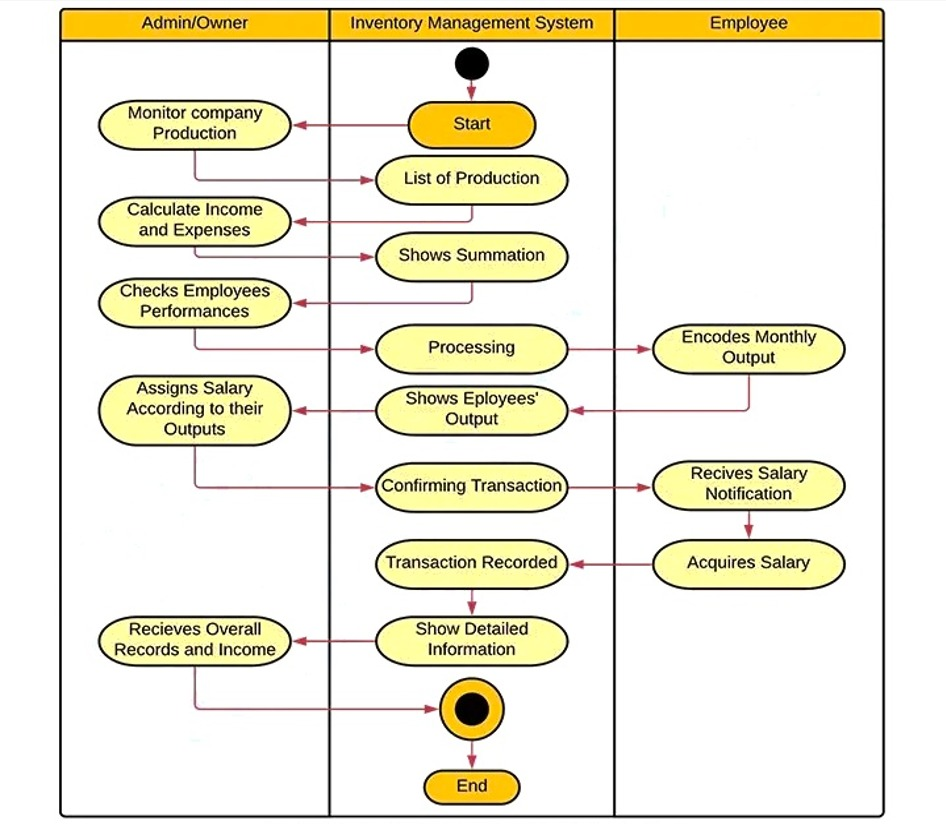
\includegraphics[width=9cm]{Figures/ActivityDiagram.jpeg}
  \caption{Activity Diagram of the system}
\label{}
\end{figure}

\begin{figure}[H]
  \centering
   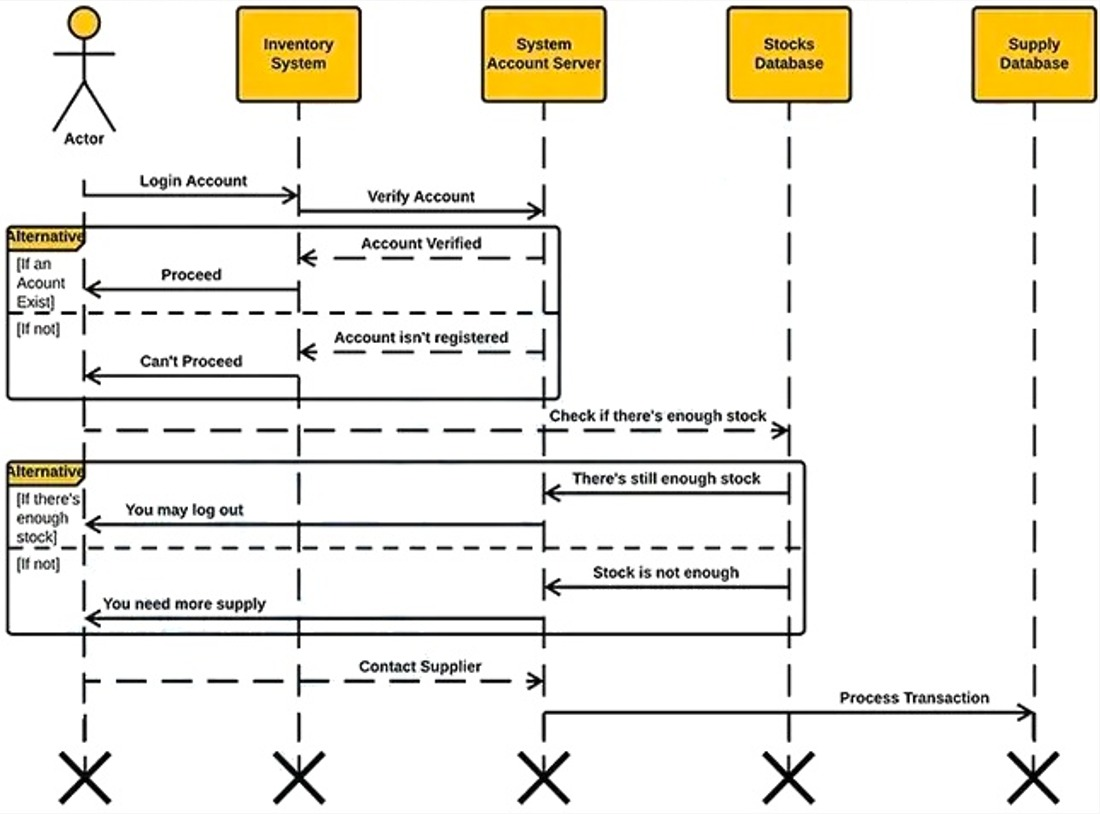
\includegraphics[width=9cm]{Figures/SequenceDiagram.jpeg}
  \caption{Sequence Diagram}
\label{}
\end{figure}

\section{Modes of operation \label{Section::Modesofoperation}}

\begin{enumerate}

    \item Online mode: Allows real-time access to inventory data through a web-based interface.

    \item Offline mode: Enables offline access to inventory data with local storage capabilities, and synchronization with the online system when an internet connection is available.

    \item Mobile mode: Provides mobile access to inventory data through a mobile application that is compatible with both Android and iOS devices.

    \item API mode: Allows integration with third-party systems through RESTful APIs for data sharing and system integration.

    \item Backup and recovery mode: Ensures data backup and recovery capabilities in case of system failures, data loss, or other disruptions.
\end{enumerate}

\section{User classes and other involved personnel \label{Section::Userclassesandotherinvolvedpersonnel}}
\begin{enumerate}
    \item Store managers: Responsible for managing inventory levels, overseeing stock movements, and making purchasing decisions.

    \item Sales staff: Responsible for tracking inventory movements, processing sales transactions, and updating inventory levels in real-time.

    \item Warehouse staff: Responsible for receiving and processing incoming shipments, managing inventory levels, and preparing outgoing shipments.

    \item IT staff: Responsible for system maintenance, upgrades, and technical support for the inventory management system.

    \item Auditors: Responsible for conducting periodic audits of inventory data and transactions to ensure accuracy and compliance with regulatory requirements.

    \item Vendors: Involved in the inventory management system as suppliers of goods and services, and can access the system for order management and delivery tracking.
\end{enumerate}
\begin{figure}[H]
  \centering
   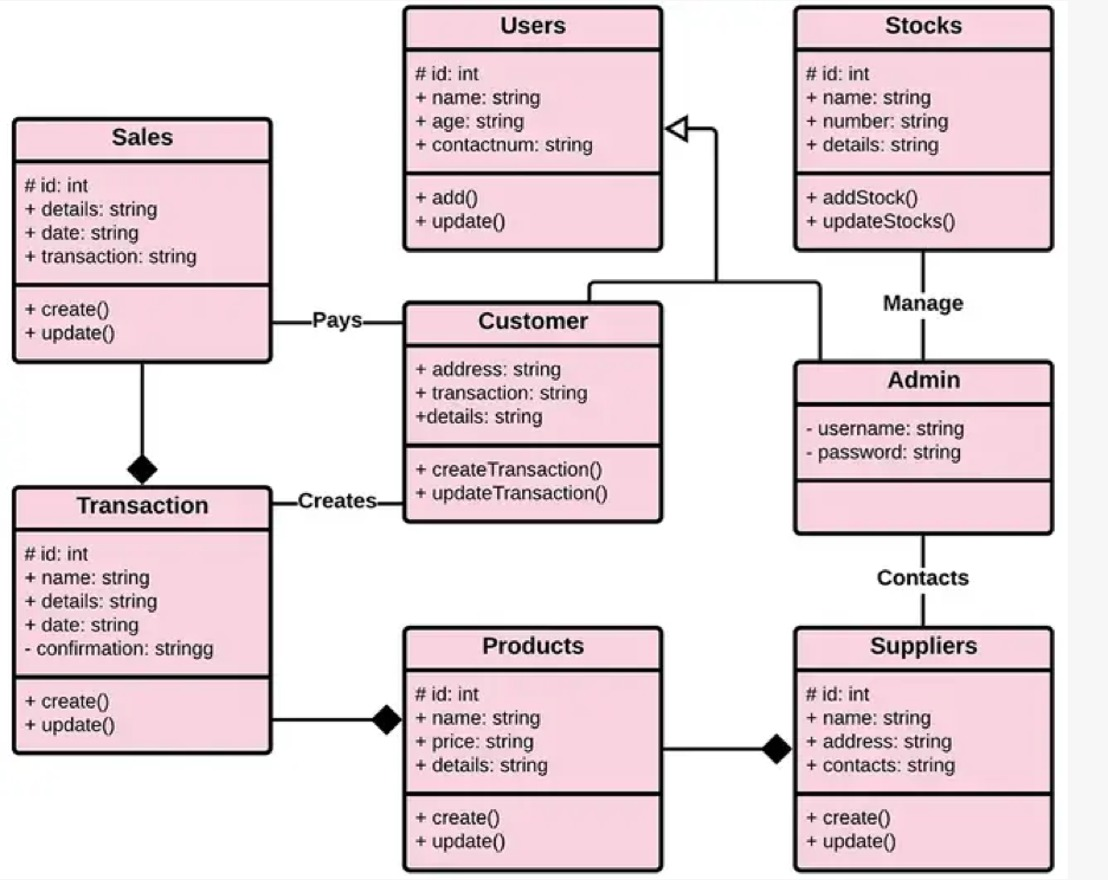
\includegraphics[width=9cm]{Figures/ClassDiagram.jpeg}
  \caption{Class Diagram of the proposed system}
\label{}
\end{figure}

\section{Support environment \label{Section::Supportenvironment}}

\begin{enumerate}
    \item Helpdesk and support services: A centralized helpdesk to provide technical support, assistance, and guidance to system users.

    \item Knowledge base and documentation: A comprehensive knowledge base and documentation system to provide users with resources and self-help tools to resolve issues and answer frequently asked questions.

    \item System maintenance and upgrades: Regular maintenance and upgrades of the system to ensure optimal performance, reliability, and security.

    \item Training and education: Training and education programs for users to ensure they have the necessary knowledge and skills to effectively use the system.

    \item User feedback and feature requests: A mechanism for users to provide feedback and suggest new features and enhancements to the system.
\end{enumerate}
\newpage
\chapter{Operational scenarios \\ 
% \small{\textit{-- Author Name}}
\index{Operational scenarios}
\label{Chapter::Operationalscenarios}} 
\begin{enumerate}
    \item Managing inventory across multiple stores: A store manager can log into the system and view inventory levels across multiple stores, transfer inventory between stores as needed, and receive alerts for low inventory levels or stockouts.


\begin{figure}[H]
  \centering
   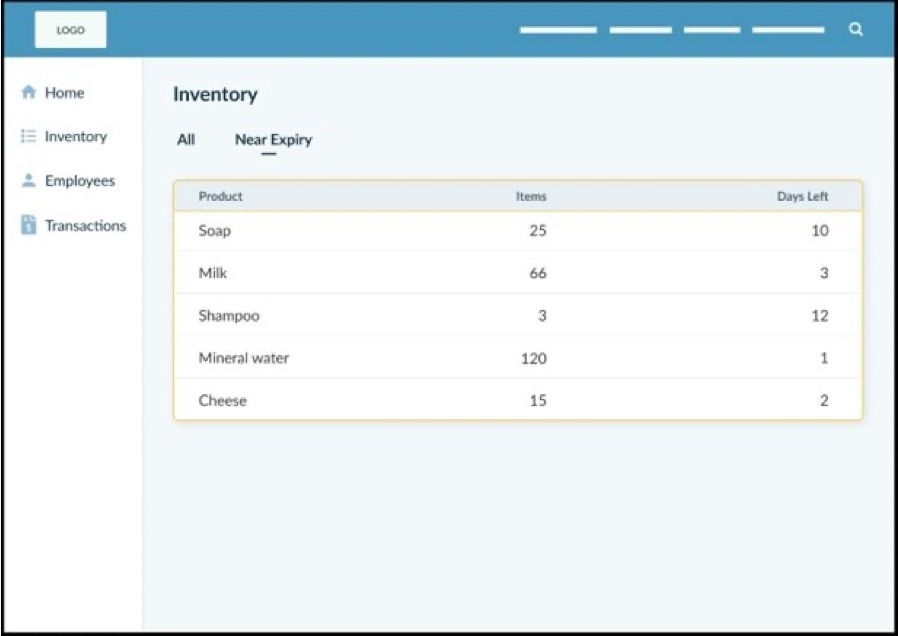
\includegraphics[width=9cm]{Figures/Figma2.jpeg}
  \caption{Inventory tab in the system}
\label{}
\end{figure}

    \item Mobile access for inventory management: A store employee can use the mobile app to access inventory data, update inventory levels, and perform inventory management tasks from anywhere, allowing for more flexibility in managing inventory.

    \begin{figure}[H]
  \centering
   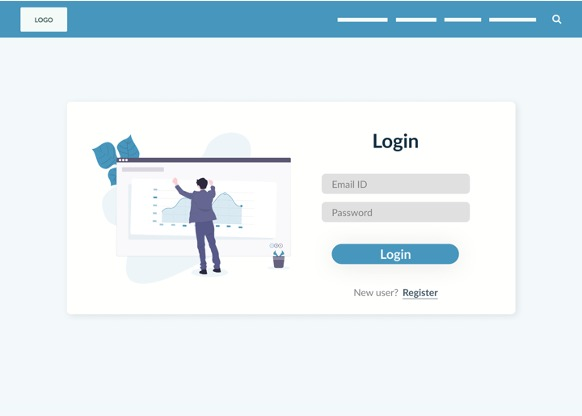
\includegraphics[width=9cm]{Figures/Figma4.jpeg}
  \caption{Login page}
\label{}
\end{figure}

\begin{figure}[H]
  \centering
   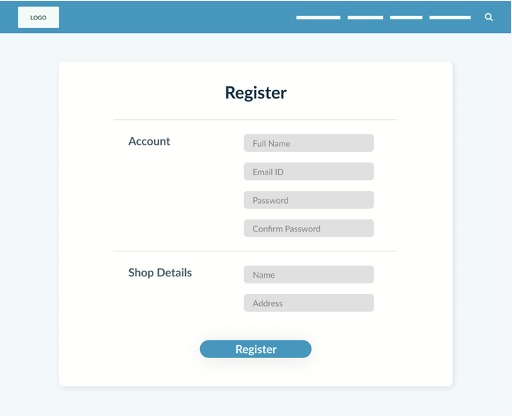
\includegraphics[width=9cm]{Figures/Figma3.jpeg}
  \caption{Registration Page}
\label{}
\end{figure}

\begin{figure}[H]
  \centering
   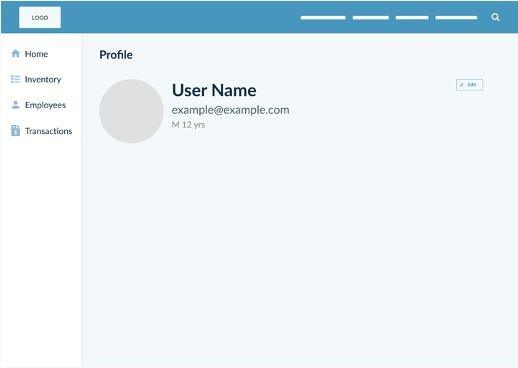
\includegraphics[width=9cm]{Figures/Figma6.jpeg}
  \caption{User profile}
\label{}
\end{figure}

    \item Customizable alerts for inventory issues: A store manager can set up customizable alerts for low inventory levels, stockouts, and other inventory-related issues, receiving notifications via email, SMS, or in-app notifications.

    
    \begin{figure}[H]
  \centering
   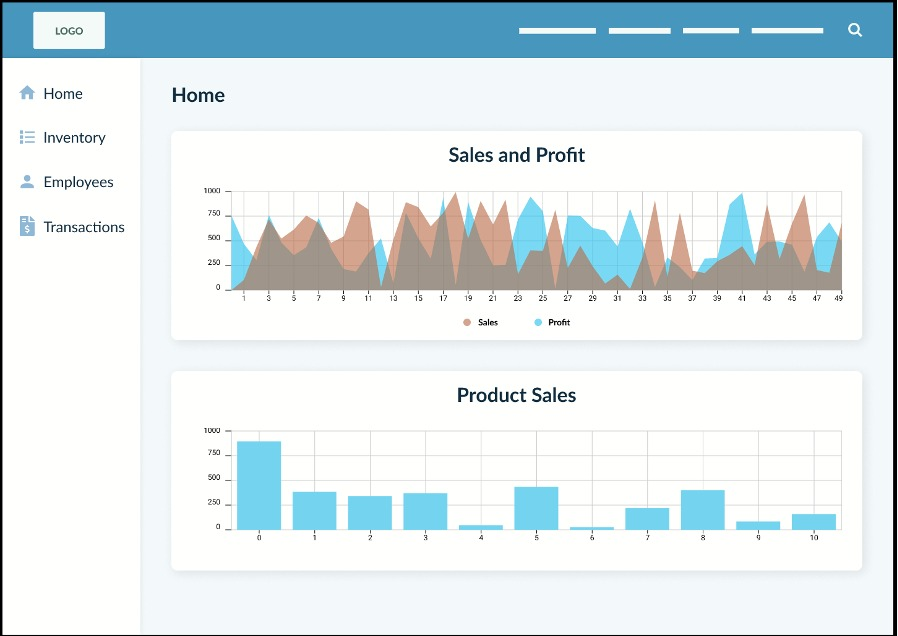
\includegraphics[width=9cm]{Figures/Figma1.jpeg}
  \caption{Homepage of the system}
\label{}
\end{figure}

    \item Automatic updates based on sales transactions: When a customer makes a purchase using the POS system, the inventory management system automatically updates inventory levels, ensuring accurate inventory tracking and reducing errors related to manual data entry.

    \begin{figure}[H]
  \centering
   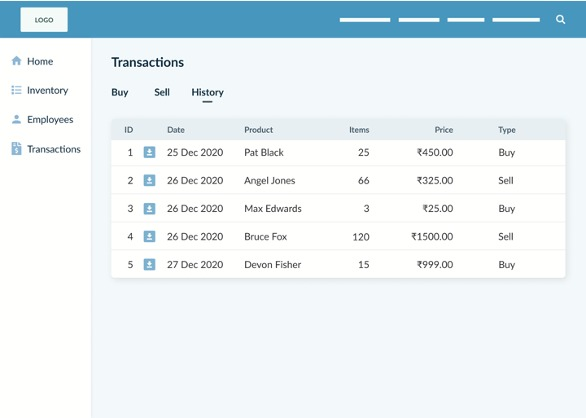
\includegraphics[width=9cm]{Figures/Figma7.jpeg}
  \caption{Transactions History tab}
\label{}
\end{figure}

\begin{figure}[H]
  \centering
   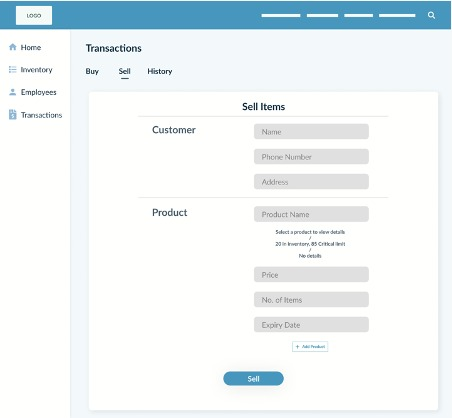
\includegraphics[width=9cm]{Figures/Figma8.jpeg}
  \caption{Transaction Details for selling items}
\label{}
\end{figure}

\begin{figure}[H]
  \centering
   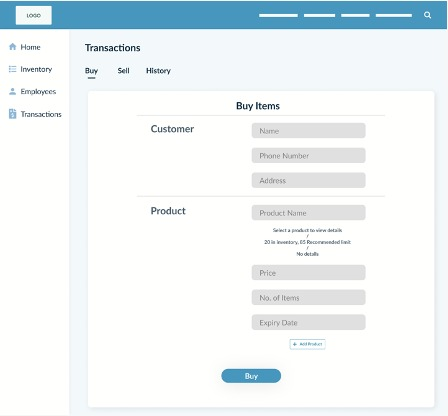
\includegraphics[width=9cm]{Figures/Figma5.jpeg}
  \caption{Transaction Details for buying items}
\label{}
\end{figure}

    \item Managing vendor relationships: A store manager can use the vendor management functionality to track vendor performance, manage purchase orders, and ensure timely delivery of goods, improving the efficiency of the purchasing process and reducing inventory-related issues.
\end{enumerate}
\newpage
\chapter{Summary of impacts \\ 
% \small{\textit{-- Author Name}}
\index{Summary of impacts}
\label{Chapter::Summaryofimpacts}} 
\section{Operational impacts \label{Section::Operationalimpacts}}
\begin{enumerate}
    \item Centralized inventory control: The ability to manage inventory across multiple stores in a centralized manner will lead to greater efficiency and accuracy in inventory tracking and management.

    \item Mobile access: The ability to access inventory data and perform inventory management tasks remotely will increase flexibility and enable more efficient use of staff time.

    \item Customizable alerts: The ability to receive alerts for low inventory levels, stockouts, and other inventory-related issues will improve inventory management and reduce the risk of stockouts and overstocking.

    \item Integration with POS system: The integration of the inventory management system with the point-of-sale system will ensure that inventory levels are automatically updated based on sales transactions, reducing errors and improving accuracy.

    \item Vendor management: The inclusion of vendor management functionality will streamline the purchasing process and improve vendor relationships, leading to more timely delivery of goods and better inventory management.
\end{enumerate}
\section{Organizational impacts \label{Section::Organizationalimpacts}}
\begin{enumerate}
    \item Improved inventory accuracy: The proposed system's automatic updates and centralized inventory control will improve inventory accuracy, reducing errors related to manual data entry and providing more accurate inventory data.

    \item Increased efficiency: Mobile access, customizable alerts, and vendor management functionality will increase the efficiency of inventory management tasks, allowing store managers and staff to manage inventory more quickly and easily.

    \item Reduced costs: Improved inventory accuracy and efficiency will reduce costs associated with overstocking, stockouts, and other inventory-related issues. Additionally, vendor management functionality can help optimize the purchasing process and reduce costs associated with late or incorrect deliveries.
\end{enumerate}

\section{Impacts during development \label{Section::Impactsduringdevelopment}}
\begin{enumerate}
    \item Time and resource requirements: Developing the proposed system will require a significant investment of time and resources, including software development, hardware procurement, and staff training.

    \item Potential disruptions to current operations: The development process may disrupt current inventory management processes, especially if the new system requires changes to existing workflows or data management practices.

    \item Collaboration and communication: Developing the proposed system will require collaboration and communication between developers, project managers, store managers, and other stakeholders to ensure that the system meets their needs and is properly integrated into their workflows.

    \item Technical challenges: The development process may encounter technical challenges, including software bugs, hardware failures, or integration issues with other systems.
\end{enumerate}

\noindent
The technical challenges can be tracked and planned around by utilizing a Bug reporting and job management software. We propose the use of JIRA.
\begin{figure}[H]
  \centering
   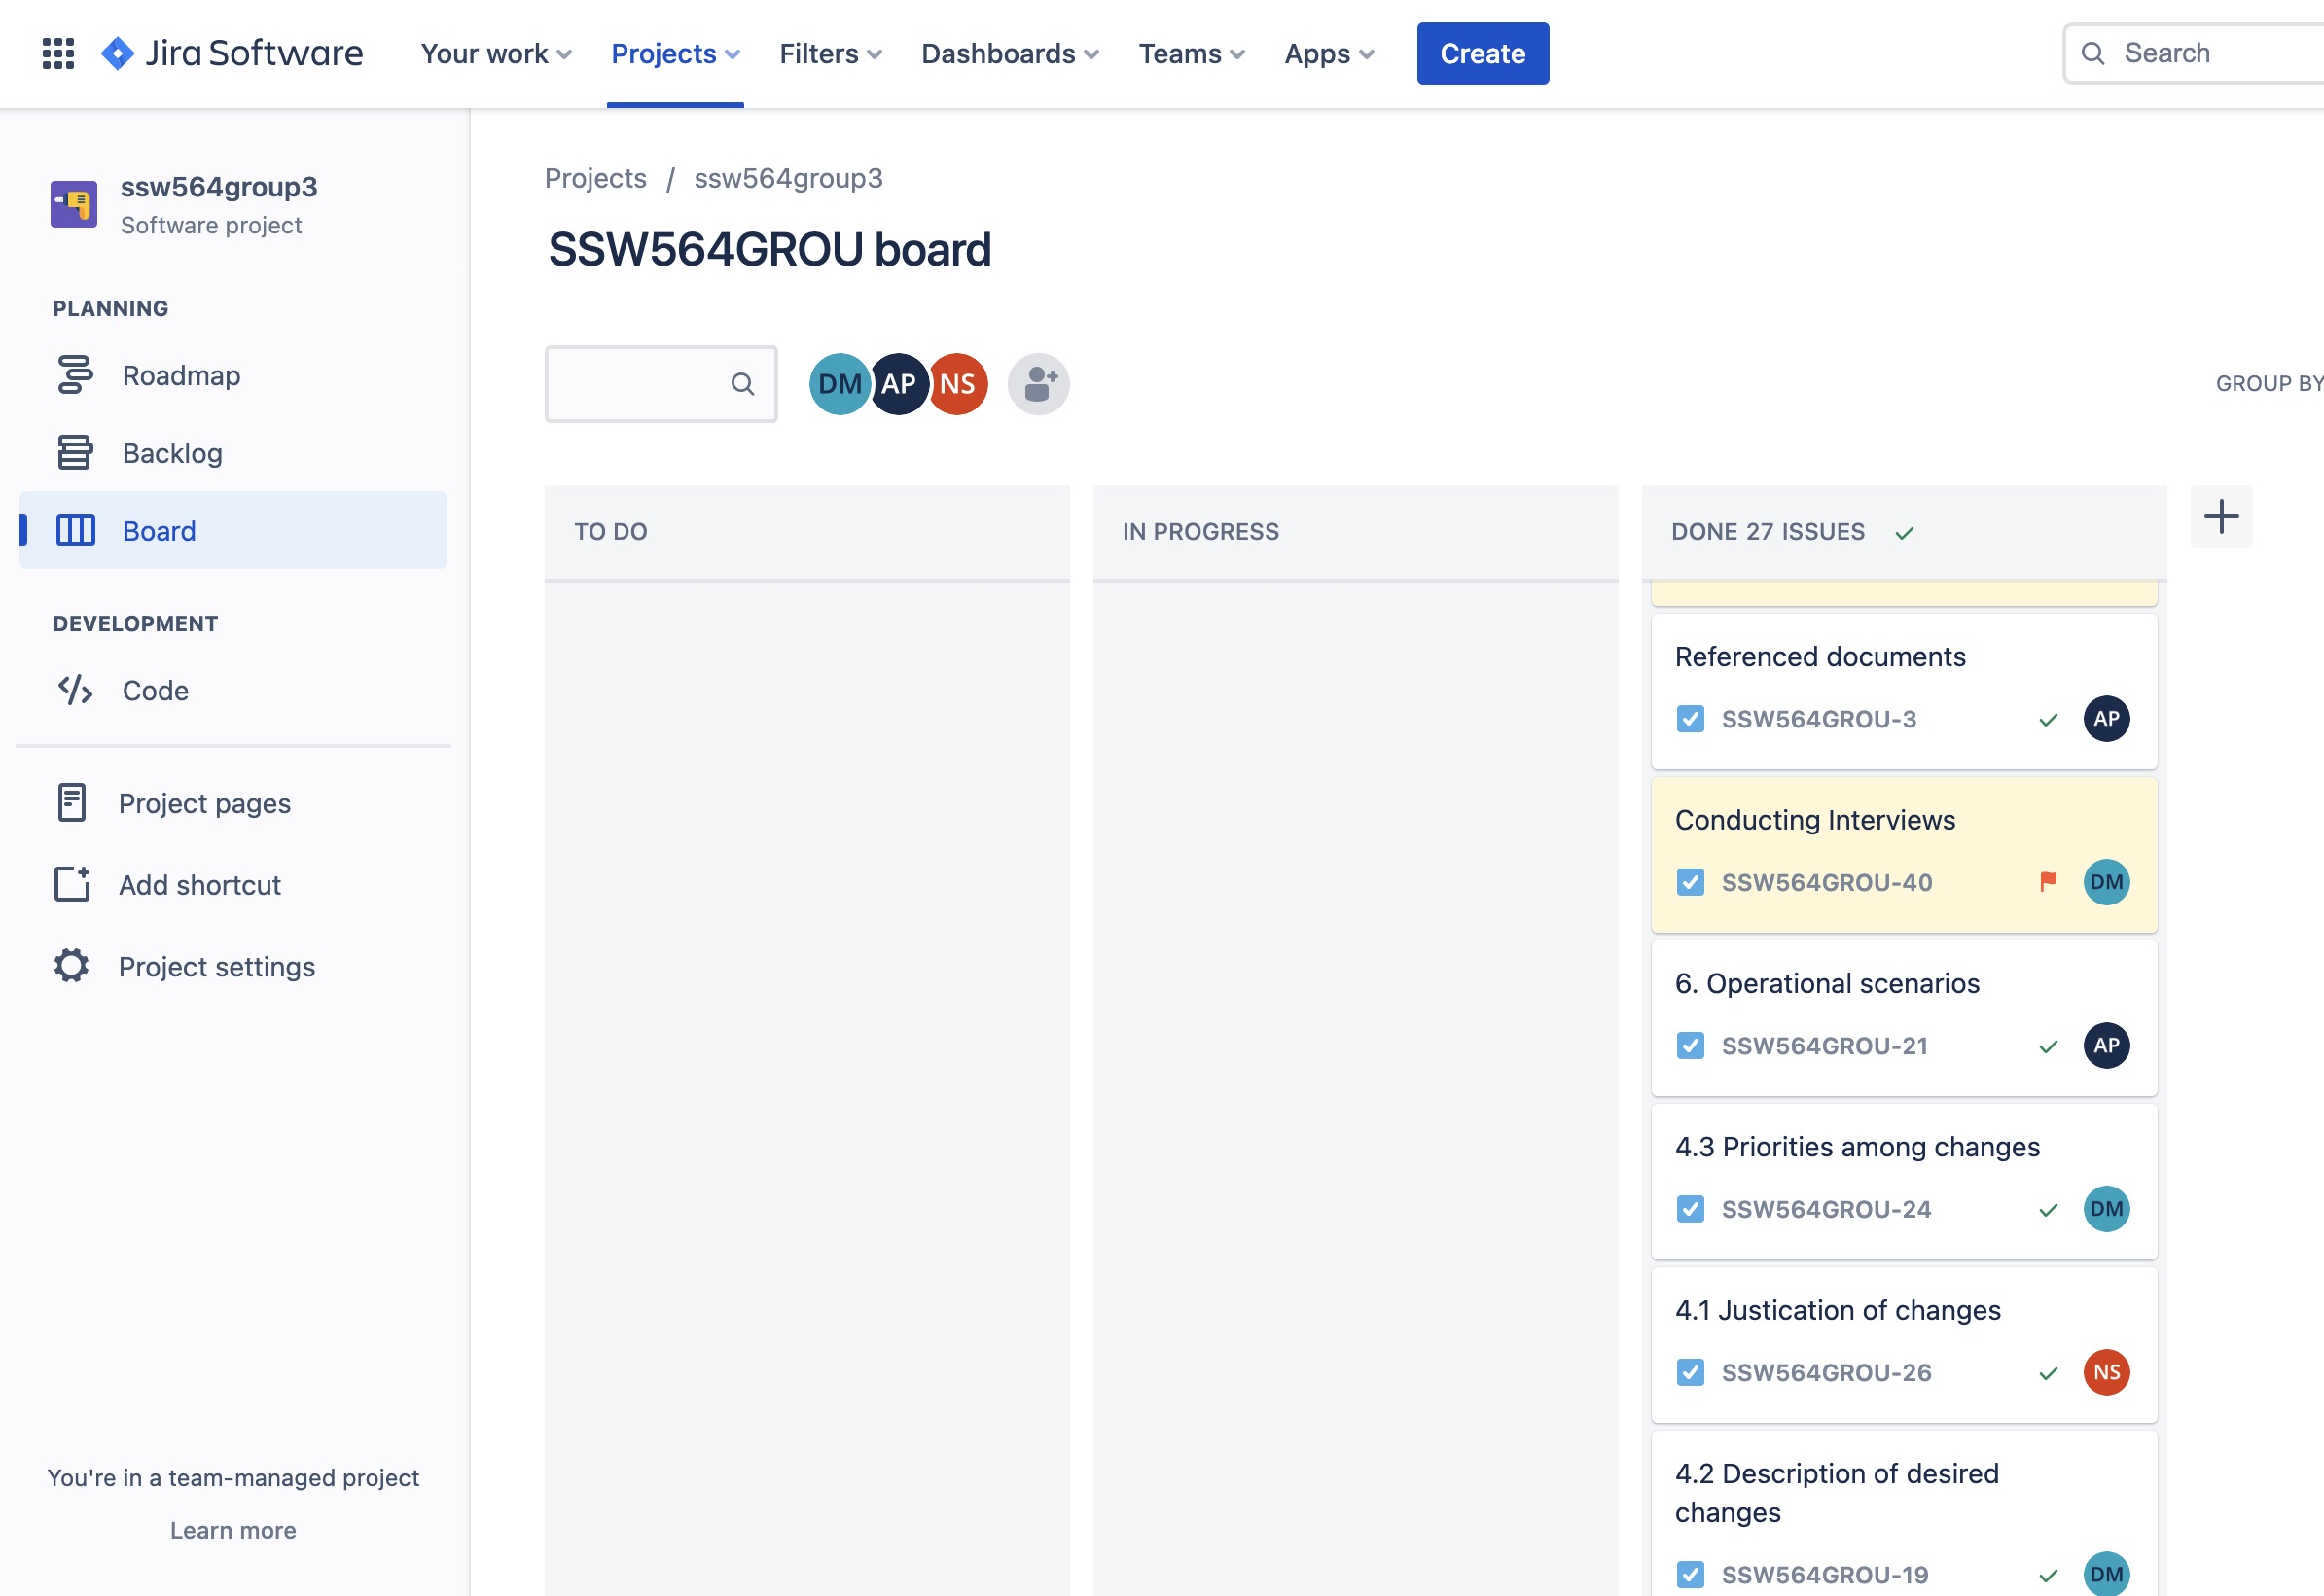
\includegraphics[width=9cm]{Figures/0DA589D3-1556-4FB9-9B0C-23CCDA029EBB_1_201_a.jpeg}
  \caption{Jira Homepage created for the project}
\label{}
\end{figure}
\newpage
\chapter{Analysis of the proposed system \\ 
% \small{\textit{-- Author Name}}
\index{Analysis of the proposed system}
\label{Chapter::Analysisoftheproposedsystem}}
\section{Summary of improvements \label{Section::Summaryofimprovements}}
\begin{enumerate}
    \item Multi-store support: The proposed system will allow for centralized inventory control across multiple locations, enabling inventory transfers between stores.

    \item Mobile access: The proposed system will provide mobile access, allowing for remote inventory management and reducing the need for physical presence in the store.

    \item Customizable alerts: The proposed system will enable customizable alerts to notify store managers and staff of low inventory levels, stockouts, and other inventory-related issues.

    \item Integration with POS system: The proposed system will integrate with the point-of-sale (POS) system, automatically updating inventory levels based on sales transactions, reducing errors related to manual data entry.

    \item Vendor management: The proposed system will include vendor management functionality, allowing for the optimization of the purchasing process and timely delivery of goods.
\end{enumerate}
\noindent
Overall, the proposed system will improve inventory accuracy, increase efficiency, and reduce costs, making it a worthwhile investment.

\section{Disadvantages and limitations \label{Section::Disadvantagesandlimitations}}
\begin{enumerate}


    \item Cost: Developing and implementing the proposed system will require a significant investment of time and resources, including software development, hardware procurement, and staff training.

    \item Technical challenges: The development and implementation of the proposed system may encounter technical challenges, including software bugs, hardware failures, or integration issues with other systems.

    \item Organizational change: The proposed system may require changes to existing workflows or data management practices, which may be disruptive and require staff training.

    \item Security concerns: Storing inventory data in a centralized system may pose security risks if not properly secured.
\end{enumerate}

\section{Alternatives and trade-offs considered \label{Section::Alternativesandtradeoffsconsidered}}
\begin{enumerate}
    \item Even though our system tries to fill in the gaps that are present in the market, the cost of doing that still remains unless and until the system scales and more retailers join, the cost of the system may remain high.
    \item To initially keep the system simple, we decided to keep english as the primary language used in the system. While, we have seen that many of the users may not be well versed with a particular language. However, this ensures a faster development of the initial product in english while later extending support to other languages.
    \item Targeted use of Cloud increases the maintenance and upfront cost of the system, however, in the long run it ensures that the system has higher availability and better scalability.
    \item Incorporation of the system may require changes to the existing workflow as in the initial software versions are designed with specific workflows in mind. Again to ensure a smoother initial release. This workflow is the one that we found to be the most commonly used.
    \item Incorporation of an advanced prediction system for forecasting inventory was considered but the resources required for it may make the system unfeasible. Thus, it should not be a part of the main system. 
\end{enumerate}
\newpage
\chapter{Notes \\ 
% \small{\textit{-- Author Name}}
\index{Notes}
\label{Chapter::Notes}}

\section{Project Mission Statement \label{Section::projectmissionstatement}}
\section{Key Stakeholders \label{Section::keystakeholders}}
\section{Key Drivers \label{Section::keydrivers}}
\section{Key Constraints \label{Section::keyconstraints}}
\section{Key Requirements \label{Section::keyrequirements}}
\section{Requirement Elicitation \label{Section::requirementelicitation}}
\section{Requirement Validation and Analysis \label{Section::requirementvalidationandanalysis}}
\section{Users \label{Section::users}}
\section{JIRA \label{Section::jira}}
\section{GitHub \label{Section::github}}
\begin{itemize}    
    \item The system does not take into account the any mishaps or exceptions in the process unless explicitly informed about it as no sensors are information collection systems are incorporated.
    \item The system may not be compliant to certain regional regulations and may need some customization for operations in such regions.
\end{itemize}

\bibliography{bibfile}
%\bibliographystyle{unsrt}
\bibliographystyle{IEEEtran}

%% Initial version by Darian Muresan, Ph.D.
% Edit and adjust as needed.

\documentclass[12pt]{cornell}

% add index support
\makeindex

% graphing programs
\usepackage{color}
\usepackage{psfrag}
\usepackage{verbatim}
\usepackage{fancyhdr}
%\usepackage{titlesec}
\usepackage{fancyvrb} 
% hyperlink programs
\usepackage[pdfmark, 
breaklinks=true, 
colorlinks=true,
citecolor=blue,
linkcolor=blue,
menucolor=black,
pagecolor=black,
urlcolor=blue
]{hyperref} % links in pdf
%\usepackage[colorlinks]{hyperref} % links in dvi
\usepackage{listings}
\usepackage{amsfonts} 
\usepackage{amssymb} 
%\usepackage{tabto}

\usepackage{tabularx,colortbl}
\usepackage[chapter]{algorithm} 
\usepackage{algorithmic} 
\usepackage{blindtext}
\usepackage{imakeidx}


\definecolor{DarkGreen}{rgb}{0,0.6,0}
\definecolor{mygreen}{rgb}{0,0.6,0}
\definecolor{mygray}{rgb}{0.5,0.5,0.5}
\definecolor{mymauve}{rgb}{0.58,0,0.82}

\usepackage{tocloft}
\usepackage{amsmath}
\usepackage{tcolorbox}
\usepackage{enumitem}
\usepackage{longtable}
%\usepackage{textcomp}
\usepackage{txfonts}

%part for \part titles
%chap for \chapter titles
%sec for \section titles
%subsec for \subsection titles
%subsubsec for \subsubsection titles
%para for \paragraph titles
%subpara for \subparagraph titles
%fig for figure \caption titles
%subfig for subfigure \caption titles
%tab for table \caption titles
%subtab for subtable \caption titles

% update chapter number spacing
\setlength{\cftchapnumwidth}{2em}
\setlength{\cftsecnumwidth}{2.5em}
\setlength{\cftsubsecnumwidth}{3.5em}
\setlength{\cftsubsubsecnumwidth}{4.5em}

\addtolength{\cftsecindent}{0.5em}
\addtolength{\cftsubsecindent}{0.5em}
\addtolength{\cftsubsubsecindent}{0.5em}

%\titlespacing*{\chapter}{0pt}{-50pt}{20pt}
%\titleformat{\chapter}[display]{\normalfont\huge\bfseries}{\chaptertitlename\ 
%\thechapter}{20pt}{\Huge}
%\pagestyle{fancy}
%\pagestyle{cornell}
%
%\rhead{F054-021-0172}
%\chead{Nonlinear Enhancement of Visual Target Detection (AF05-T021)}
%\lhead{GSTI}
%\lfoot{\scriptsize Use or disclosure of data on this page is subject
%to the restriction on the title page of this proposal.}
%\cfoot{}
%\rfoot{\thepage}

\newfont{\Bp}{msbm10}
\newfont{\BpBig}{msbm10 scaled\magstep2}
\newfont{\Sc}{eusm10}
\newfont{\ScBig}{eusm10 scaled\magstep3}
\newfont{\Fr}{eufm10}
\newfont{\FrBig}{eufm10 scaled\magstep1}

% some commands:
\newcommand{\dxi}{{\tt m\_xDeltaInput}}
\newcommand{\dyi}{{\tt m\_yDeltaInput}}
\newcommand{\dci}{{\tt m\_cDeltaInput}}
\newcommand{\dxo}{{\tt m\_xDeltaOutput}}
\newcommand{\dyo}{{\tt m\_yDeltaOutput}}
\newcommand{\dco}{{\tt m\_cDeltaOutput}}
\newcommand{\ttf}[1]{{\tt #1}}
\newcommand{\tbl}[2]{{\begin{tabular}{c} #1 \\ #2 \end{tabular}}}

\newcommand{\urltwo}[2]{\mbox{\href{#1}{\tt #2}}}
\newcommand{\qnorm}[1]{\|#1\|_{\bQ}}
\newcommand{\qdot}[2]{\lrb #1, #2 \rrb_{\bQ}}
\newcommand{\kdot}[2]{\lrb #1, #2 \rrb_{\bf k}}
\newcommand{\tdot}[2]{\lrb #1, #2 \rrb}
\newcommand{\mydiff}[2]{\lrb #1 - #2 \rrb}
\newcommand{\lena}{\textit{lena}}
\newcommand{\barb}{\textit{barbara}}
\newcommand{\boat}{\textit{boat}}
\newcommand{\leaves}{\textit{leaves}}
\newcommand{\rings}{\textit{rings}}
\newcommand{\treg}{\textit{train region}}
\newcommand{\dreg}{\textit{denoise region}}
\newcommand{\oreg}{\textit{overlap region}}
\newcommand{\sil}{\sigma_l^2}
\newcommand{\sn}{\sigma^2}
\newcommand{\bn}{{\mbox{\bf \FrBig N}}}
\newcommand{\n}{\mbox{\Fr N}}
%\newcommand{\bn}{\bf N}
%\newcommand{\n}{N}
\newcommand{\bY}{\textbf{Y}}
\newcommand{\bX}{\textbf{X}}
\newcommand{\bb}{\textbf{b}}
\newcommand{\bu}{\textbf{u}}
\newcommand{\bv}{\textbf{v}}
\newcommand{\by}{\textbf{y}}
\newcommand{\bx}{\textbf{x}}
\newcommand{\be}{\textbf{e}}
\newcommand{\bz}{\textbf{z}}
\newcommand{\bs}{\textbf{s}}
\newcommand{\bw}{\textbf{w}}
\newcommand{\bQ}{\textbf{Q}}
\newcommand{\bphi}{\textbf{$\phi$}}
\newcommand{\lsb}{\left[}
\newcommand{\rsb}{\right]}
\newcommand{\lrb}{\left(}
\newcommand{\rrb}{\right)}
\newcommand{\lcb}{\left\{}
\newcommand{\rcb}{\right\}}
\newcommand{\R}{\mbox{\BpBig R}}
\newcommand{\F}{{\cal F}}
\newcommand{\Fk}{\mbox{\Sc F}}
\newcommand{\bQF}{\textbf{Q}_{\mbox{\Sc F}}}
\newcommand{\N}{{\cal N}}
\newcommand{\xlz}{X_l(z)}
\newcommand{\xhz}{X_h(z)}
\newcommand{\xz}{X(z)}
\newcommand{\pr}{ perfect reconstruction }
\newcommand{\smb}{Smith-Barnwell }
\newcommand{\xw}{X(e^{j\omega})}
\newcommand{\xmw}{X(-e^{j\omega})}
\newcommand{\dw}{D(e^{j\omega})}
\newcommand{\dmw}{D(-e^{j\omega})}
\newcommand{\ew}{E(e^{j\omega})}
\newcommand{\emw}{E(-e^{j\omega})}
\newcommand{\fw}{F_0(e^{j\omega})}
\newcommand{\fmw}{F_0(-e^{j\omega})}
\newcommand{\hoz}{H_1(z)}
\newcommand{\hzz}{H_0(z)}
\newcommand{\goz}{G_1(z)}
\newcommand{\gzz}{G_0(z)}
\newcommand{\hzw}{H_{0}(e^{j\omega})}
\newcommand{\hzmw}{H_{0}(-e^{j\omega})}
\newcommand{\hzcw}{H_{0}(e^{-j\omega})}
\newcommand{\how}{H_1(e^{j\omega})}
\newcommand{\homw}{H_1(-e^{j\omega})}
\newcommand{\gzw}{G_0(e^{j\omega})}
\newcommand{\gzmw}{G_0(-e^{j\omega})}
\newcommand{\gow}{G_1(e^{j\omega})}
\newcommand{\gomw}{G_1(-e^{j\omega})}
\newcommand{\wl}{e^{-jwL}}
\newcommand{\aqua}{\textit{AQua with OR }}
\newtheorem{theorem}{Theorem}
\newtheorem{lemma}{Lemma}
\newtheorem{corollary}{Corollary}
\newtheorem{claim}{Claim}
\newtheorem{definition}{Definition}
\newenvironment{proof}{\noindent{\em Proof.}}{\ \hfill Q.E.D.}
%\newtheorem{moduleCount}{L}
\newcommand*{\labelfile}[1]{%
  \label{file:#1}%
}

\lstset{ %
  backgroundcolor=\color{white},   % choose the background color; you must add \usepackage{color} or \usepackage{xcolor}
  basicstyle=\footnotesize,        % the size of the fonts that are used for the code
  breakatwhitespace=false,         % sets if automatic breaks should only happen at whitespace
  breaklines=true,                 % sets automatic line breaking
  captionpos=b,                    % sets the caption-position to bottom
  commentstyle=\color{DarkGreen},    % comment style
  deletekeywords={...},            % if you want to delete keywords from the given language
  escapeinside={\%*}{*)},          % if you want to add LaTeX within your code
  extendedchars=true,              % lets you use non-ASCII characters; for 8-bits encodings only, does not work with UTF-8
  %frame=single,                   % adds a frame around the code
  keepspaces=true,                 % keeps spaces in text, useful for keeping indentation of code (possibly needs columns=flexible)
  keywordstyle=\color{blue},       % keyword style
  language=C++,                    % the language of the code
  morekeywords={*,...},            % if you want to add more keywords to the set
  numbers=left,                    % where to put the line-numbers; possible values are (none, left, right)
  numbersep=5pt,                   % how far the line-numbers are from the code
  numberstyle=\tiny\color{mygray}, % the style that is used for the line-numbers
  rulecolor=\color{black},         % if not set, the frame-color may be changed on line-breaks within not-black text (e.g. comments (green here))
  showspaces=false,                % show spaces everywhere adding particular underscores; it overrides 'showstringspaces'
  showstringspaces=false,          % underline spaces within strings only
  showtabs=false,                  % show tabs within strings adding particular underscores
  stepnumber=1,                    % the step between two line-numbers. If it's 1, each line will be numbered
  stringstyle=\color{mymauve}     % string literal style
  %tabsize=2,                      % sets default tabsize to 2 spaces
  %caption=\lstname                % show the filename of files included with \lstinputlisting; also try caption instead of title
}

% Uncomment draftcopy to get the word DRAFT boldly across the first page
%   By the way, xdvi won't show it but it will come out when you print
%\usepackage[light,all]{draftcopy}		% DRAFT on first page
%\draftcopySetGrey{.97}
%\draftcopyName{Confidential}{150}
%\draftcopFirstPage{1}

% Uncomment drafthead to get the date and DRAFT in the header of pages
% that are normallly numbered on the top, pages 2-n of each chapter for example
% This doesn't work with centered page numbers: \pagestyle{cornellc}
%\usepackage{drafthead}

% Including selective chapters:
% use this to selectively process chapters, etc.  Put a % in front of
% the sections that you don't want done this time.  Includes are
% used instead of \input so that LaTeX will keep track of chapters and
% pages without processing everything.  Don't let any spaces creep in
% around the words or it will not work!


\includeonly{
prologue,
manIntroduction,
Identifyprojecttitle,
Referenceddocuments,
Currentsystemorsituation,
Justificationforandnatureofchanges,
Conceptsfortheproposedsystem,
Operationalscenarios,
Summaryofimpacts,
Analysisoftheproposedsystem,
Notes

}

\makeindex

\begin{document}

\pagenumbering{roman}
\singlespacing
% File: prologue.tex
% Thesis prologue:  Title page, acknowledgements, table of contents,
% list of figures, and list of tables.
%
% this file is to be \include'd after the \begin{document}

% Cornell-style title page
\begin{titlepage}
        \title{Projects Assignments}
        \author{Ashay Pable\\Divyamshu Mandadi\\Neel Savani\\ Stevens.edu }
        \conferraldate{}{\today} \maketitle
\end{titlepage}

% Copyright page
%\begin{copyrightpage}
\makecopyright
%\end{copyrightpage}

% Abstract: the abstract body is pulled from the file abstract.tex;
%  the title is pulled from the \title command in the titlepage section
\begin{abstract}
        %\makeabstitle
        \input abstract      % puts the abstract file here
\end{abstract}

% Biographical information pulled from file bio.tex
%\begin{biosketch} \input bio \end{biosketch}

% Dedication (optional):  pulls information from file dedication.tex
%\begin{dedication} 
%\input dedicate 
%\end{dedication}

% Acknowledgements:  pulls information from file acknow
%\begin{acknowledgements} \input acknow \end{acknowledgements}

% Table of contents
\contentspage

% If you have no tables or figures put a % in front of the list page line
% List of tables
\tablelistpage

% List of figures
\figurelistpage



\setcounter{page}{1}        % set page counter
\pagenumbering{arabic}      % set page number style
\pagestyle{fancy}         % top right page numbers
%\pagestyle{cornell}
%\pagestyle{cornellc}       % centered page numbers, disables drafthead

\renewcommand{\chaptermark}[1]{\markboth{#1}{}}
\renewcommand{\sectionmark}[1]{\markright{#1}{}}

\fancyhead{} % clear all fields

\lhead{Chapter \thechapter}
%\lhead{\thechapter}
\chead{\leftmark}
\rhead{\thepage}


\lfoot{Chapter \thechapter}
\cfoot{\copyright Stevens -- \today \mbox{} -- Project Name}
\rfoot{\thepage}

\renewcommand{\headrulewidth}{0.4pt}
\renewcommand{\footrulewidth}{0.4pt}

%\rhead{F054-021-0172}
%\chead{Nonlinear Enhancement of Visual Target Detection (AF05-T021)}
%\lhead{GSTI}
%\lfoot{\scriptsize Use or disclosure of data on this page is subject
%to the restriction on the title page of this proposal.}
%\cfoot{}
%\rfoot{\thepage}


\singlespacing
% \chapter{Introduction \\
% \small{\textit{-- Author Name}} 
% % \index{Chapter!introduction}
% \index{introduction}
% \label{Chapter::Introduction}}

% \chapter{Analysis of the proposed system \\ 
% % \small{\textit{-- Author Name}}
% \index{Analysis of the proposed system}
% \label{Chapter::Analysisoftheproposedsystem}}

% % Add a section and label it so that we can reference it later
% \section{My Section \label{Section::MySection}}


% % add a new page
% \newpage

% Hi there world!  Here is an example of a note\footnote{Here is a reference 
% to Figure \ref{Figure::manAgile} and an indexed keyword\index{keyword}.}

\chapter{Identify project and Mission statement \\
% \small{\textit{-- Ashay Pable}} 
%\index{Chapter!Homework One -- Requirements}
\index{Identify project and Mission statement}
\label{Chapter::Identify project and Mission statement}}

% Add a section and label it so that we can reference it later
\section{Team Members \label{Section::teamMembers}}
\begin{enumerate}
  \item \textbf{Ashay Pable} : I am a Masters in Software Engineering student. I have worked as a software
developer for 4 years in India with a wide range of experience from Artificial Intelligence to
3D Graphics development. I have a keen interest in automation powered by AI and research
in contributing fields. My experience as a developer has made me realise the importance of
planning and documentation before initiation of a project
  \item \textbf{Divyamshu Mandadi} : My name is Divyamshu Mandadi and I’m currently in my third
semester doing my Masters in Software Engineering. Before moving to the US I have
worked as a Software Developer in India. My experience while working there combined
with the curiosity to learn more about the Software development processes led me here.
  \item \textbf{Neel Savani} : My name is Neel Savani. I had completed my under-graduation in Informa-
tion and Technology at birla vishwakarma mahavidhyalaya. I am currently in my second-
semester pursuing my masters in Software engineering. I am interested in developing soft-
ware.
\end{enumerate}

\section{Team Name \label{Section::teamName}}
"Group 3 - Inventory Management System for Retail Stores"
\section{Project Chosen \label{Section::projectChosen}}
\begin{itemize}
 \item Inventory Management system for Retail Stores.
 \item The project's goal is to create an intuitive and efficient inventory management system that will provide a retail business with real-time visibility into inventory levels and movement.
\end{itemize}
\section{Project Mission Statement \label{Section::projectMissionStatement}}
Our mission is to provide seamless and continuous supply of inventory so that customers needs are catered to in an efficient manner. Our system will provide an intuitive user interface that enables efficient recording and management of each item in the inventory. Retailers will be able to minimize stockouts, manage inventory levels for maximum profitability, and base data-driven choices on real-time inventory levels. This system provides a comprehensive solution that improves inventory management for retail establishments, frees up time, reduces expenses, and increases overall operational performance.

% \cite{GM1998}.

%\begin{figure}
%\centering
%\scalebox{0.8}{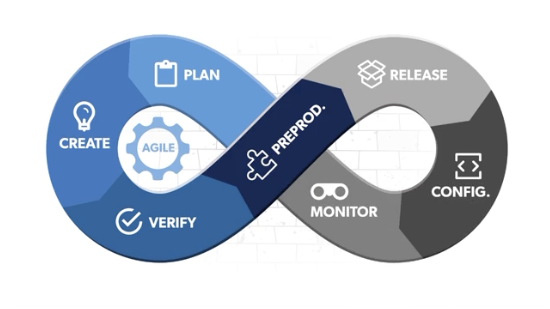
\includegraphics{Figures/manAgileProcess.png}}
%\caption{\label{Figure::manAgile} Figure of the continuous agile process.}
%\end{figure}

% add a new page
\newpage

\chapter{Referenced documents \\ 
% \small{\textit{-- Author Name}}
\index{Referenced documents}
\label{Chapter::Referenceddocuments}} 

Several recent studies, relevant research papers and articles with keywords such as “Inventory Management” and “Retail” or “Retail Sector” and “Operations Research” Databases such as Google Scholar, Science Direct and Z-library were also used. We also used Oracle Retail Store Inventory Management Documentation Library extensively to identify their features, limitations and how through our system we can mitigate them.\cite{ORACLE}

\newpage
\chapter{Current system or situation \\ 
% \small{\textit{-- Author Name}}
\index{Current system or situation}
\label{Chapter::Currentsystemorsituation}} 
\section{Background, objectives, and scope \label{Section::Backgroundobjectivesandscope}}
The instore inventory management system is an essential tool for managing inventory in a retail store. The system is responsible for tracking the movement of goods, monitoring stock levels, and ensuring that the right products are available at the right time. The current manual inventory management system is time-consuming, prone to errors, and lacks real-time visibility of inventory levels. The new instore inventory management system aims to address these challenges by automating the process, providing accurate and real-time inventory information, and enabling efficient and effective management of inventory levels.
The primary objective of the instore inventory management system is to improve the accuracy, efficiency, and effectiveness of inventory management in the retail store. Specifically, the system aims to achieve the following objectives:
\begin{enumerate}    
\item Real-time inventory visibility: Provide accurate and real-time visibility of inventory levels to store managers and staff.

\item Automated inventory tracking: Automate the process of tracking inventory movement, including receiving, stocking, and selling products.

\item Efficient inventory management: Enable efficient management of inventory levels, including setting reorder points, managing stock levels, and reducing waste.

\item Improved decision-making: Provide data analytics and reporting tools to support informed decision-making related to inventory management.
\end{enumerate}
The instore inventory management system will be designed to manage inventory for a single retail store. The system will be integrated with the existing point-of-sale (POS) system to provide real-time inventory information. The system will track the movement of goods from the time they are received into the store until they are sold or removed from inventory. The system will include features for setting reorder points, generating purchase orders, and monitoring stock levels. The system will also include reporting and data analytics tools to support informed decision-making related to inventory management.

The system will be designed to be user-friendly and intuitive to use, with minimal training required for store managers and staff. The system will be scalable, allowing for the addition of new products and the expansion of the store. The system will be designed to be compatible with existing hardware and software systems in the store. Finally, the system will be secure and reliable, ensuring the confidentiality and integrity of inventory data.

\section{Operational policies and constraints \label{Section::Operationalpoliciesandconstraints}}

\textbf{Operational policies:}
\begin{enumerate}
\item Access control: Access to the instore inventory management system will be restricted to authorized personnel only. Access credentials will be assigned on a need-to-know basis.
\item Data protection: The system will store inventory data in a secure and encrypted manner. Data backups will be taken regularly to ensure data integrity and availability in case of system failure.
\item Maintenance and support: The system will be maintained and supported by trained personnel to ensure optimal performance and reliability. Maintenance schedules will be developed to minimize disruptions to store operations.
\item Training and documentation: Store managers and staff will be provided with adequate training and documentation to ensure proper use of the system. Training will be ongoing, and documentation will be updated as needed.
\item Change management: Changes to the system, including upgrades and modifications, will be managed through a formal change management process. Changes will be tested and validated before implementation.

\end{enumerate}

\noindent
\textbf{Constraints:}
\begin{enumerate}
\item Budget: The implementation of the instore inventory management system will be subject to budgetary constraints. The cost of hardware, software, and personnel will need to be within the allocated budget.

\item Integration with existing systems: The system will need to be integrated with the existing point-of-sale (POS) system, which may have limitations on compatibility.

\item Technical limitations: The system will be subject to technical limitations, such as hardware capacity and bandwidth limitations.

\item User adoption: The success of the system will depend on the adoption by store managers and staff. The system will need to be user-friendly and intuitive to ensure adoption.

\item Regulatory compliance: The system will need to comply with all relevant regulatory requirements, including data privacy and security regulations.
\end{enumerate}

\section{Description of the current system or situation \label{Section::Descriptionofthecurrentsystemorsituation}}
The current inventory management system in the retail store is a manual process that is time-consuming and prone to errors. The process involves tracking inventory movement, monitoring stock levels, and placing orders for replenishment. The system relies on physical counts, spreadsheets, and manual record-keeping to track inventory.

The process begins with the receipt of goods from suppliers. The store manager or staff checks the goods against the purchase order and records the receipt in a manual log. The goods are then moved to the storage area, and the stock level is updated manually.

When items are sold, the store manager or staff records the sale in the point-of-sale (POS) system and manually updates the inventory count. When stock levels fall below a certain threshold, the store manager or staff manually creates a purchase order to replenish the inventory.

The current system has several limitations. Firstly, the manual process is time-consuming and prone to errors, leading to inaccurate inventory counts and stockouts. Secondly, the system lacks real-time visibility of inventory levels, making it challenging to manage stock levels effectively. Finally, the manual process does not provide data analytics and reporting tools to support informed decision-making related to inventory management.\cite{OR2020}
\begin{figure}[H]
  \centering
   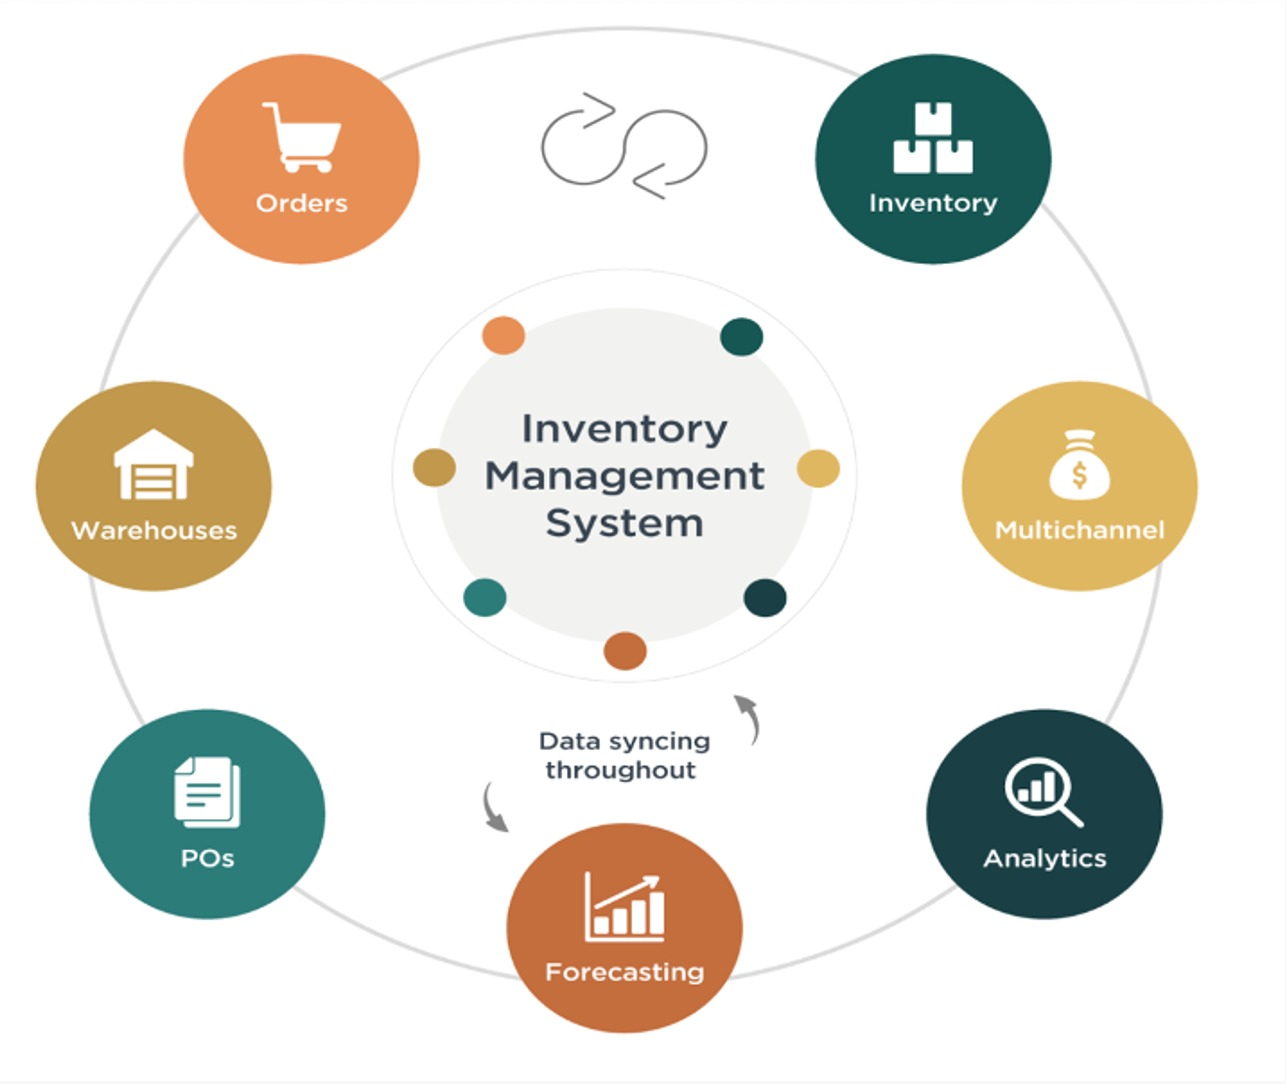
\includegraphics[width=9cm]{Figures/SpiritDiagram.jpeg}
  \caption{Overview Diagram}
\label{}
\end{figure}
\section{Modes of operation for the current system or situation \label{Section::Modesofoperationforthecurrentsystemorsituation}}
The current inventory management system in the retail store operates in the following modes:

\begin{enumerate}
    
\item Receiving mode: This mode is activated when goods are received from suppliers. The store manager or staff checks the goods against the purchase order and records the receipt in a manual log. The goods are then moved to the storage area, and the stock level is updated manually.

\item Stocking mode: This mode is activated when goods are moved from the storage area to the shelves or display areas. The store manager or staff manually updates the inventory count.

\item Selling mode: This mode is activated when items are sold to customers. The store manager or staff records the sale in the point-of-sale (POS) system and manually updates the inventory count.

\item Ordering mode: This mode is activated when stock levels fall below a certain threshold. The store manager or staff manually creates a purchase order to replenish the inventory.

\end{enumerate}

The current system operates in a sequential manner, with each mode depending on the previous mode's completion. The system lacks real-time visibility of inventory levels and does not provide automated inventory tracking or reporting tools.

\section{User classes and other involved personnel \label{Section::Userclassesandotherinvolvedpersonnel}}
The following are the user classes and other personnel involved in the instore inventory management system:

\begin{enumerate}

    \item Store manager: The store manager is responsible for managing the inventory and overseeing the instore inventory management system's operation. The store manager is responsible for setting up the system, assigning access credentials to authorized personnel, and ensuring the system's proper use.


    \item Store staff: The store staff is responsible for handling the goods, updating inventory levels, and generating reports using the instore inventory management system. The store staff will be provided with adequate training and documentation to ensure proper use of the system.

    \item IT personnel: The IT personnel will be responsible for    installing, configuring, and maintaining the hardware and software components of the system. They will also be responsible for ensuring the system's security, integrity, and availability.

    \item Suppliers: The suppliers will be involved in the system through the receipt of purchase orders generated by the system. The suppliers will need to ensure timely delivery of goods and accurate order fulfillment.

    \item Customers: The customers indirectly interact with the system by purchasing goods that are managed by the instore inventory management system. The system will ensure that the customers have access to the products they need when they need them, improving their shopping experience.
    
\end{enumerate}

The involvement of these user classes and personnel is critical to the success of the instore inventory management system, and their cooperation and support will be essential for the system's effective implementation and operation.

\section{Support environment \label{Section::Supportenvironment}}
\begin{enumerate}
    \item Help desk: A help desk will be set up to provide support and assistance to store managers and staff using the system. The help desk will be staffed by trained personnel who can provide technical assistance and troubleshooting support.

    \item Online documentation: The instore inventory management system will include online documentation that provides detailed instructions on how to use the system's features and functionality. The documentation will be regularly updated and available online for easy access.

    \item Training sessions: Store managers and staff will be provided with adequate training on the system's operation and functionality. Training sessions will be conducted both online and in-person and will be tailored to the specific needs of the user class.

    \item Maintenance and support team: A dedicated maintenance and support team will be responsible for ensuring the system's optimal performance and reliability. The team will be available to respond to system issues and perform maintenance tasks as required.

    \item Vendor support: The system vendor will provide technical support and assistance in case of system issues or malfunctions. The vendor will be responsible for ensuring that the system operates as intended and meets the user's requirements.
    
\end{enumerate}


\newpage
\chapter{Justification for and nature of changes \\ 
% \small{\textit{-- Author Name}}
\index{Justification for and nature of changes}
\label{Chapter::Justificationforandnatureofchanges}} 
\section{Justication of changes \label{Section::Justicationofchanges}}
The justification for these changes is to address several key issues identified through a recent analysis of our company's operations. This analysis revealed a number of inefficiencies and bottlenecks that have been negatively impacting productivity and profitability. The proposed changes aim to streamline workflows, improve communication and collaboration, and optimize resource allocation to achieve better results.

\noindent
There are several reasons why changes are required, including:

\begin{enumerate}

    \item New business requirements: The business requirements for the instore inventory management system may change as the business grows or as market conditions change. These changes may require modifications to the system to support new requirements.

    \item Technological advancements: Advancements in technology may provide new opportunities to improve the system's performance, reliability, and scalability. These advancements may require changes to the system to take advantage of the new capabilities.

    \item User feedback: Feedback from users may reveal areas where the system could be improved to better meet their needs. This feedback may prompt changes to the system's design or functionality.

    \item Regulatory requirements: Changes in regulatory requirements may require modifications to the system to ensure compliance with new regulations.

    \item External factors: External factors, such as changes in the competitive landscape or economic conditions, may require modifications to the system to remain competitive or to reduce costs.

\end{enumerate}

The nature of changes in the instore inventory management system can range from minor modifications to major overhauls. Changes may involve adding new functionality, modifying existing functionality, or removing functionality that is no longer required. Changes may also involve modifications to the system's architecture or infrastructure to improve performance, reliability, or scalability.


\section{Description of desired changes \label{Section::Descriptionofdesiredchanges}}
The instore inventory management system requires several changes to enhance its performance, reliability, and scalability. Some of the desired changes are:

\begin{enumerate}

    \item Multi-store support: The system will now support multiple stores, enabling store managers and staff to manage inventory across several locations. This change will provide centralized inventory control and enable inventory transfers between stores, reducing the risk of stockouts or overstocking.

    \item Mobile access: The system will now provide mobile access, allowing store managers and staff to access inventory data and perform inventory management tasks from anywhere at any time. This change will enable remote inventory management and reduce the need for physical presence in the store, increasing efficiency and reducing costs.

    \item Customizable alerts: The system will now enable customizable alerts that notify store managers and staff of low inventory levels, stockouts, and other inventory-related issues. These alerts can be customized to specific thresholds and sent via email, SMS, or in-app notifications. This change will help ensure timely inventory management and reduce the risk of stockouts or overstocking.

    \item Integration with POS system: The system will now integrate with the point-of-sale (POS) system, allowing inventory levels to be automatically updated based on sales transactions. This change will ensure accurate inventory tracking and reduce errors related to manual data entry.

    \item Vendor management: The system will now include vendor management functionality, enabling store managers and staff to manage vendor relationships and track vendor performance. This change will help optimize the purchasing process and ensure timely delivery of goods, reducing the risk of stockouts or overstocking.
    
\end{enumerate}
These changes will improve the system's functionality and make it more user-friendly, efficient, and accurate. The system will provide multi-store support, mobile access, customizable alerts, integration with the POS system, and vendor management functionality, enabling store managers and staff to manage inventory efficiently and effectively across multiple stores.

\section{Priorities among changes \label{Section::Prioritiesamongchanges}}
The priorities of the desired changes for the inventory management system would depend on the specific needs of the product. However, general benefits are:

\begin{enumerate}

    \item Integration with POS system: Integrating the inventory management system with the point-of-sale (POS) system should be a top priority as it would enable automatic inventory updates based on sales transactions. This would ensure accurate inventory tracking, reduce errors related to manual data entry, and provide real-time visibility into inventory levels.

    \item Customizable alerts: Implementing customizable alerts should be a high priority as it would notify store managers and staff of low inventory levels, stockouts, and other inventory-related issues, enabling timely inventory management and reducing the risk of stockouts or overstocking.

    \item Mobile access: Providing mobile access to the inventory management system should also be a high priority as it would enable store managers and staff to access inventory data and perform inventory management tasks from anywhere at any time, increasing efficiency and reducing costs.

    \item Vendor management: Including vendor management functionality should be a moderate priority as it would help optimize the purchasing process and ensure timely delivery of goods, reducing the risk of stockouts or overstocking.

    \item Multi-store support: Implementing multi-store support should be a moderate priority as it would enable store managers and staff to manage inventory across multiple locations, providing centralized inventory control and enabling inventory transfers between stores.

\end{enumerate}
Prioritizing these changes would enable the organization to implement the most critical improvements first and progressively enhance the system's functionality and efficiency over time.

\section{Changes considered but not included \label{Section::Changesconsideredbutnotincluded}}
During the development of the proposed instore inventory management system, several changes may have been considered but not included for various reasons. May be in a future iteration these can be incorporated. Some of these changes may include:

\begin{enumerate}
    \item RFID Technology: The use of RFID technology to track inventory in real-time is an option that may have been considered. However, this technology can be expensive to implement, and it may not be feasible for smaller organizations with limited resources.

    \item Advanced Artificial Intelligence: The use of artificial intelligence to automate inventory management tasks and make more accurate predictions have been considered. However, this technology can be complex and may require significant resources to implement and maintain. This will require a certain scale of operation before it may become profitable. Meanwhile, systems with lesser accuracy may suffice.

    \item Automatic Reorder: Automatic reorder functionality can be used to automatically generate purchase orders when inventory levels fall below a certain threshold. However, this feature involves a high risk factor and utilizing this without thorough testing and establishment may taint the products image in the market.

    \item Custom Barcode Generation: Barcode generation functionality can be used to generate barcodes for inventory items. However, This system may not be necessary as most products already come with a unique barcode. It is done only in case of threat with regards to barcode tampering, which only happens when the suppliers are non trusted entities, which is extremely rare.

\end{enumerate}

\newpage
\chapter{Concepts for the proposed system \\ 
% \small{\textit{-- Author Name}}
\index{Concepts for the proposed system}
\label{Chapter::Conceptsfortheproposedsystem}} 
\section{Background, objectives, and scope \label{Section::Backgroundobjectivesandscope}}
\begin{enumerate}
    
    \item Multi-store support: The system will support multiple stores, allowing store managers and staff to manage inventory across multiple locations. This will provide centralized inventory control and enable inventory transfers between stores.

    \item Mobile access: The system will provide mobile access, allowing store managers and staff to access inventory data and perform inventory management tasks from anywhere at any time. This will enable remote inventory management and reduce the need for physical presence in the store.

    \item Customizable alerts: The system will enable customizable alerts that notify store managers and staff of low inventory levels, stockouts, and other inventory-related issues. Alerts can be customized to specific thresholds and sent via email, SMS, or in-app notifications.

    \item Integration with POS system: The system will integrate with the point-of-sale (POS) system, allowing inventory levels to be automatically updated based on sales transactions. This will ensure accurate inventory tracking and reduce errors related to manual data entry.

    \item Vendor management: The system will include vendor management functionality, allowing store managers and staff to manage vendor relationships and track vendor performance. This will help optimize the purchasing process and ensure timely delivery of goods.

\end{enumerate}

\section{Operational policies and constraints \label{Section::Operationalpoliciesandconstraints}}
\textbf{Operational policies}:
\begin{enumerate}
    \item Access control: Access to the instore inventory management system will be restricted to authorized personnel only. Access credentials will be assigned on a need-to-know basis.

    \item Data protection: The system will store inventory data in a secure and encrypted manner. Data backups will be taken regularly to ensure data integrity and availability in case of system failure.

    \item Maintenance and support: The system will be maintained and supported by trained personnel to ensure optimal performance and reliability. Maintenance schedules will be developed to minimize disruptions to store operations.

    \item Training and documentation: Store managers and staff will be provided with adequate training and documentation to ensure proper use of the system. Training will be ongoing, and documentation will be updated as needed.

    \item Change management: Changes to the system, including upgrades and modifications, will be managed through a formal change management process. Changes will be tested and validated before implementation.
\end{enumerate}
\textbf{Constraints}:
\begin{enumerate}
    \item Budget: The implementation of the instore inventory management system will be subject to budgetary constraints. The cost of hardware, software, and personnel will need to be within the allocated budget.

    \item Integration with existing systems: The system will need to be integrated with the existing point-of-sale (POS) system, which may have limitations on compatibility.

    \item Technical limitations: The system will be subject to technical limitations, such as hardware availability and bandwidth limitations as the system may need to be operated in remote areas where connectivity is scarce.

    \item User adoption: The success of the system will depend on the adoption by store managers and staff. The system will need to be user-friendly and intuitive to ensure adoption.

    \item Regulatory compliance: The system will need to comply with all relevant regulatory requirements, including data privacy and security regulations.
\end{enumerate}
\section{Description of the proposed system \label{Section::Descriptionoftheproposedsystem}}

The proposed instore inventory management system is a web-based software solution designed to help retailers and store managers manage their inventory more efficiently and effectively. The system will include the following key features:

\begin{enumerate}
    \item Multi-store support: Supports multiple stores with centralized inventory control and transfers between stores.

    \item Mobile access: Provides mobile access for remote inventory management.

    \item Customizable alerts: Enables customizable alerts for low inventory levels and other inventory-related issues.

    \item Integration with POS system: Integrates with POS system for automatic inventory updates.

    \item Vendor management: Includes vendor management functionality for managing vendor relationships and tracking performance.

    \item Reporting and analytics: Provides real-time reporting and analytics for data-driven decision making.

    \item User roles and permissions: Has different user roles and permissions for authorized access and data security.

    \item Security and data privacy: Ensures security and privacy of inventory data and user information with robust security features.
\end{enumerate}
The proposed instore inventory management system will provide retailers and store managers with a comprehensive solution for managing their inventory more efficiently and effectively. It will enable centralized inventory control, remote inventory management, and real-time reporting and analytics to help optimize inventory management strategies and improve overall store performance.

\begin{figure}[H]
  \centering
   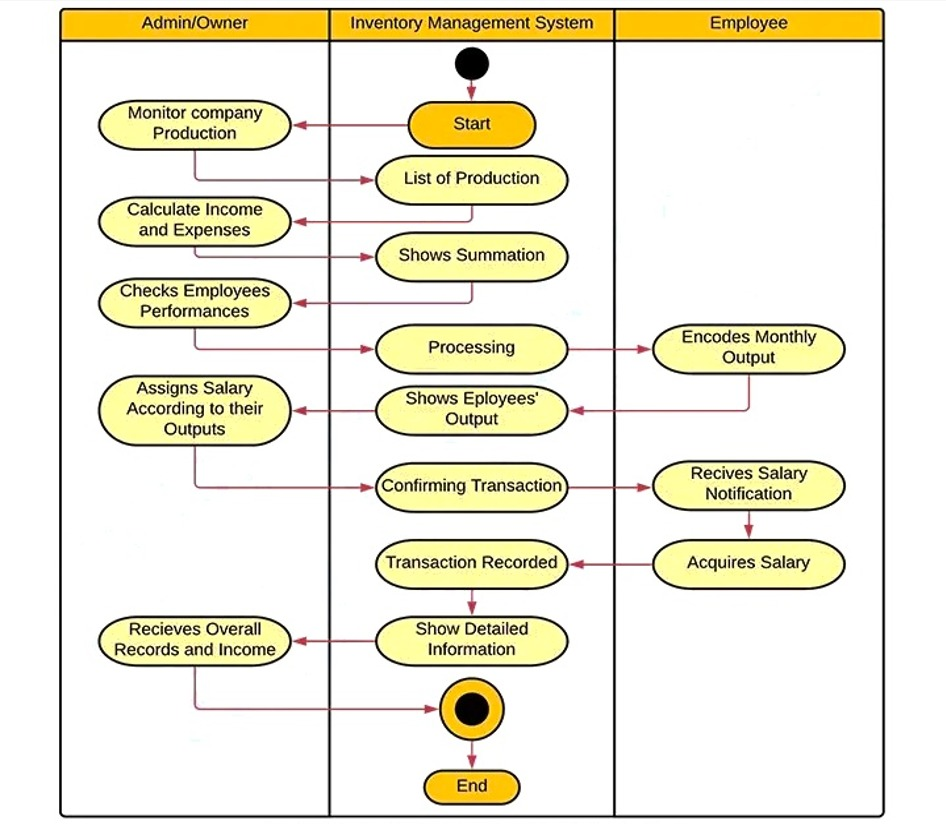
\includegraphics[width=9cm]{Figures/ActivityDiagram.jpeg}
  \caption{Activity Diagram of the system}
\label{}
\end{figure}

\begin{figure}[H]
  \centering
   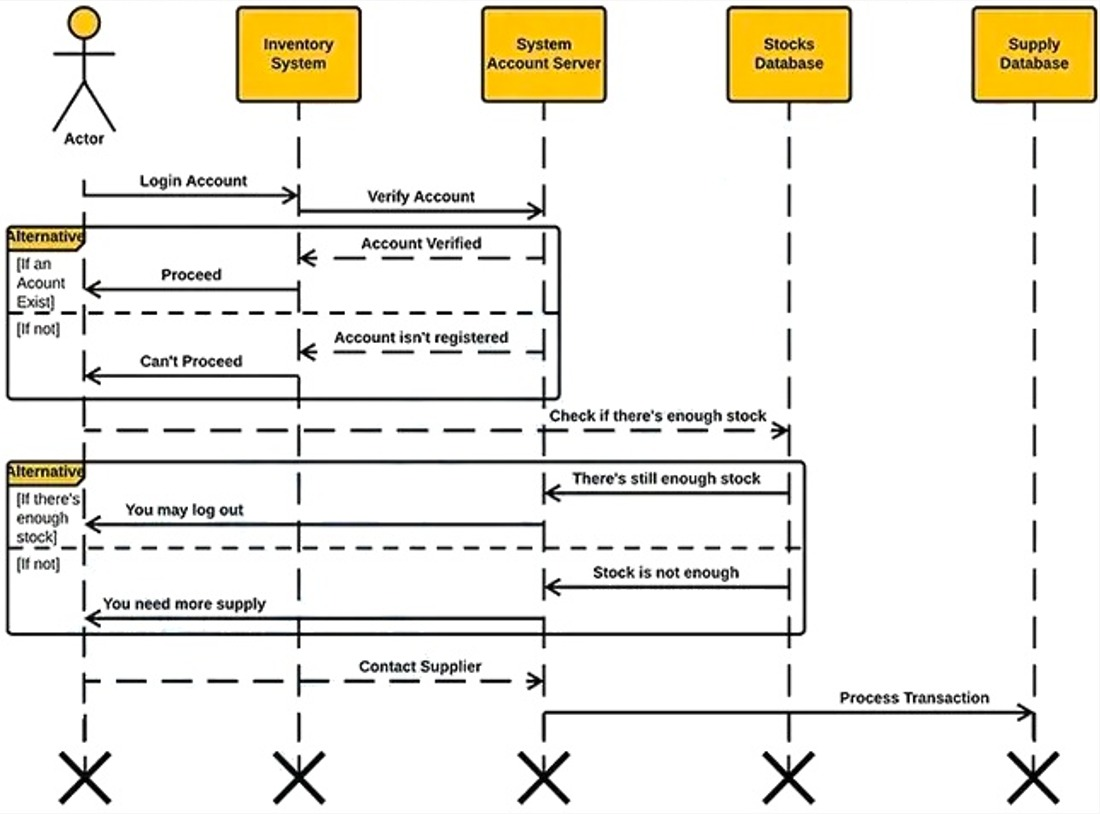
\includegraphics[width=9cm]{Figures/SequenceDiagram.jpeg}
  \caption{Sequence Diagram}
\label{}
\end{figure}

\section{Modes of operation \label{Section::Modesofoperation}}

\begin{enumerate}

    \item Online mode: Allows real-time access to inventory data through a web-based interface.

    \item Offline mode: Enables offline access to inventory data with local storage capabilities, and synchronization with the online system when an internet connection is available.

    \item Mobile mode: Provides mobile access to inventory data through a mobile application that is compatible with both Android and iOS devices.

    \item API mode: Allows integration with third-party systems through RESTful APIs for data sharing and system integration.

    \item Backup and recovery mode: Ensures data backup and recovery capabilities in case of system failures, data loss, or other disruptions.
\end{enumerate}

\section{User classes and other involved personnel \label{Section::Userclassesandotherinvolvedpersonnel}}
\begin{enumerate}
    \item Store managers: Responsible for managing inventory levels, overseeing stock movements, and making purchasing decisions.

    \item Sales staff: Responsible for tracking inventory movements, processing sales transactions, and updating inventory levels in real-time.

    \item Warehouse staff: Responsible for receiving and processing incoming shipments, managing inventory levels, and preparing outgoing shipments.

    \item IT staff: Responsible for system maintenance, upgrades, and technical support for the inventory management system.

    \item Auditors: Responsible for conducting periodic audits of inventory data and transactions to ensure accuracy and compliance with regulatory requirements.

    \item Vendors: Involved in the inventory management system as suppliers of goods and services, and can access the system for order management and delivery tracking.
\end{enumerate}
\begin{figure}[H]
  \centering
   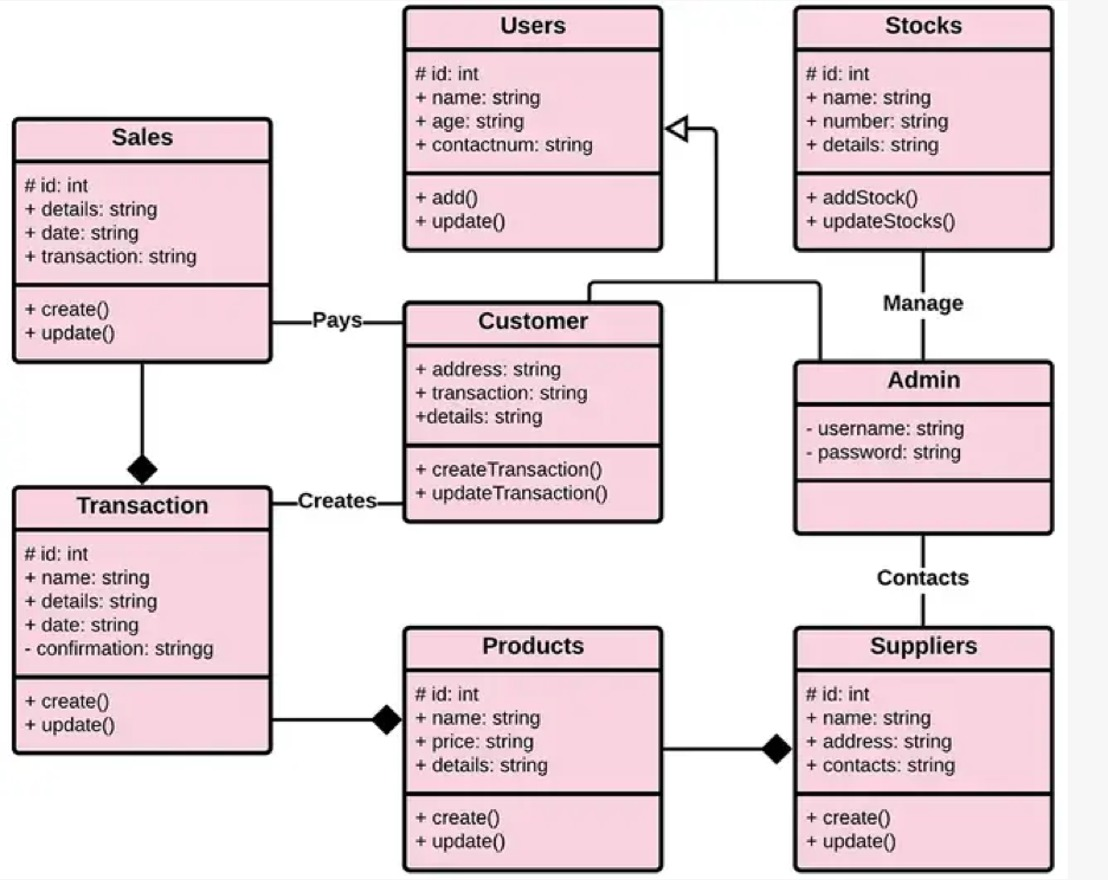
\includegraphics[width=9cm]{Figures/ClassDiagram.jpeg}
  \caption{Class Diagram of the proposed system}
\label{}
\end{figure}

\section{Support environment \label{Section::Supportenvironment}}

\begin{enumerate}
    \item Helpdesk and support services: A centralized helpdesk to provide technical support, assistance, and guidance to system users.

    \item Knowledge base and documentation: A comprehensive knowledge base and documentation system to provide users with resources and self-help tools to resolve issues and answer frequently asked questions.

    \item System maintenance and upgrades: Regular maintenance and upgrades of the system to ensure optimal performance, reliability, and security.

    \item Training and education: Training and education programs for users to ensure they have the necessary knowledge and skills to effectively use the system.

    \item User feedback and feature requests: A mechanism for users to provide feedback and suggest new features and enhancements to the system.
\end{enumerate}
\newpage
\chapter{Operational scenarios \\ 
% \small{\textit{-- Author Name}}
\index{Operational scenarios}
\label{Chapter::Operationalscenarios}} 
\begin{enumerate}
    \item Managing inventory across multiple stores: A store manager can log into the system and view inventory levels across multiple stores, transfer inventory between stores as needed, and receive alerts for low inventory levels or stockouts.


\begin{figure}[H]
  \centering
   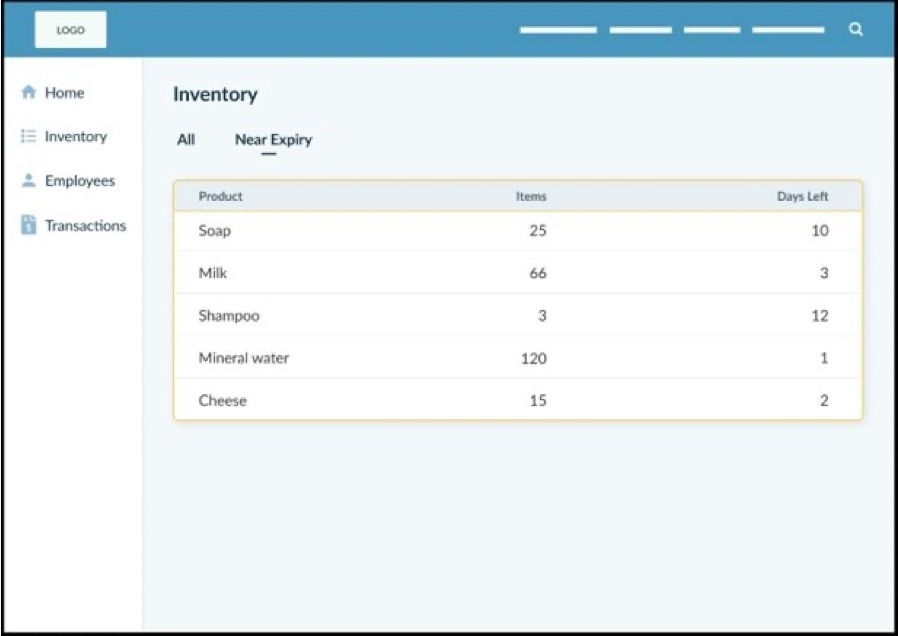
\includegraphics[width=9cm]{Figures/Figma2.jpeg}
  \caption{Inventory tab in the system}
\label{}
\end{figure}

    \item Mobile access for inventory management: A store employee can use the mobile app to access inventory data, update inventory levels, and perform inventory management tasks from anywhere, allowing for more flexibility in managing inventory.

    \begin{figure}[H]
  \centering
   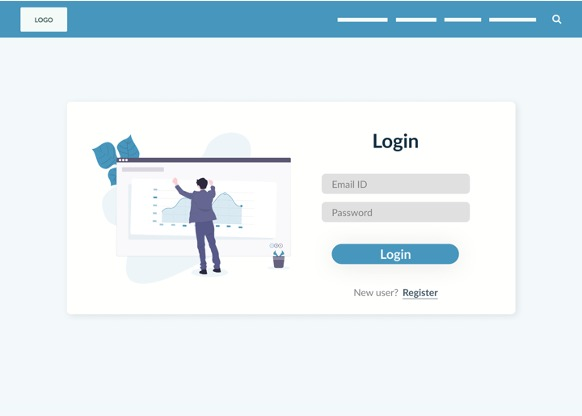
\includegraphics[width=9cm]{Figures/Figma4.jpeg}
  \caption{Login page}
\label{}
\end{figure}

\begin{figure}[H]
  \centering
   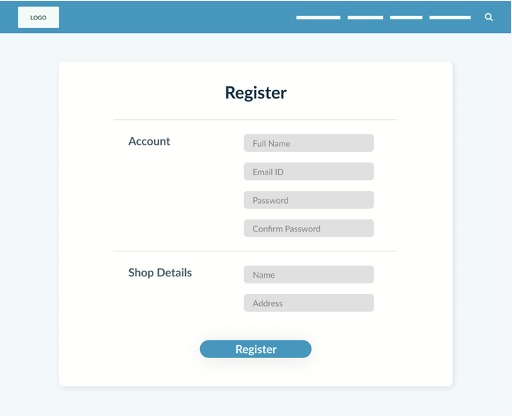
\includegraphics[width=9cm]{Figures/Figma3.jpeg}
  \caption{Registration Page}
\label{}
\end{figure}

\begin{figure}[H]
  \centering
   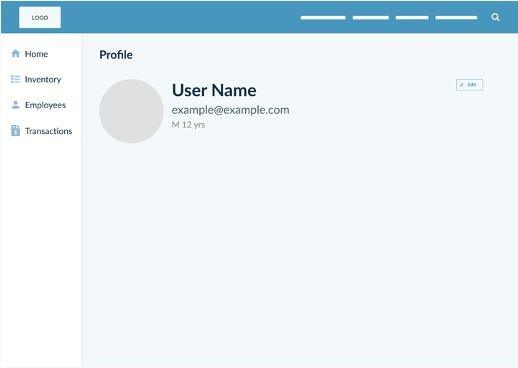
\includegraphics[width=9cm]{Figures/Figma6.jpeg}
  \caption{User profile}
\label{}
\end{figure}

    \item Customizable alerts for inventory issues: A store manager can set up customizable alerts for low inventory levels, stockouts, and other inventory-related issues, receiving notifications via email, SMS, or in-app notifications.

    
    \begin{figure}[H]
  \centering
   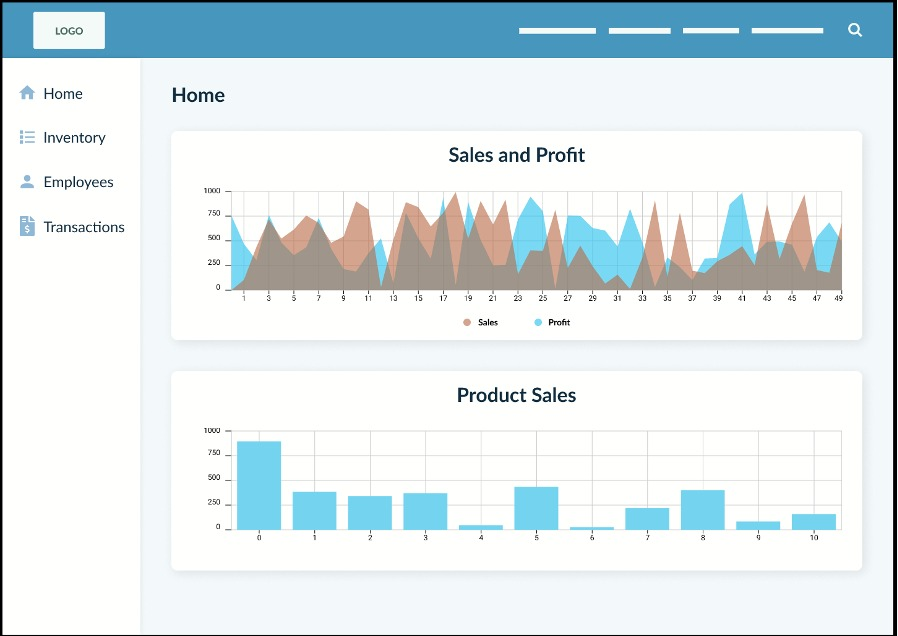
\includegraphics[width=9cm]{Figures/Figma1.jpeg}
  \caption{Homepage of the system}
\label{}
\end{figure}

    \item Automatic updates based on sales transactions: When a customer makes a purchase using the POS system, the inventory management system automatically updates inventory levels, ensuring accurate inventory tracking and reducing errors related to manual data entry.

    \begin{figure}[H]
  \centering
   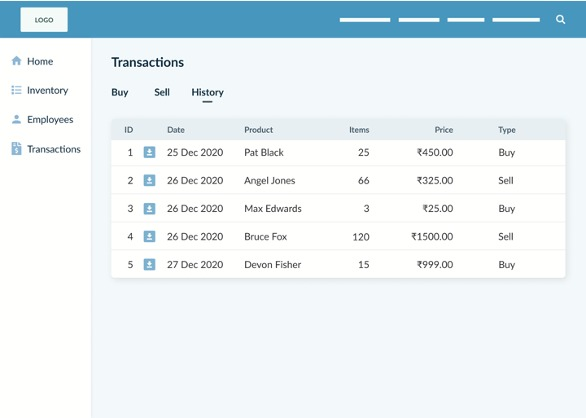
\includegraphics[width=9cm]{Figures/Figma7.jpeg}
  \caption{Transactions History tab}
\label{}
\end{figure}

\begin{figure}[H]
  \centering
   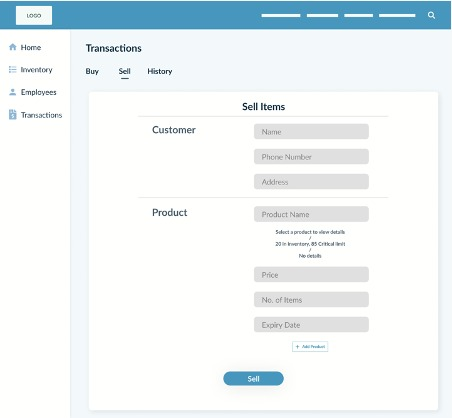
\includegraphics[width=9cm]{Figures/Figma8.jpeg}
  \caption{Transaction Details for selling items}
\label{}
\end{figure}

\begin{figure}[H]
  \centering
   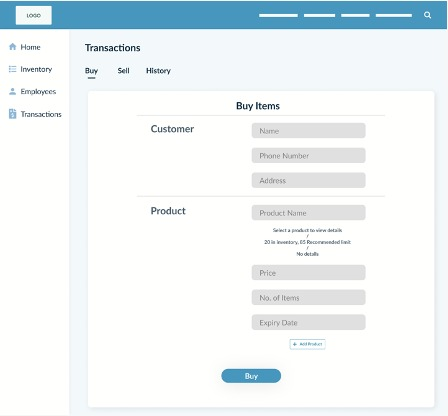
\includegraphics[width=9cm]{Figures/Figma5.jpeg}
  \caption{Transaction Details for buying items}
\label{}
\end{figure}

    \item Managing vendor relationships: A store manager can use the vendor management functionality to track vendor performance, manage purchase orders, and ensure timely delivery of goods, improving the efficiency of the purchasing process and reducing inventory-related issues.
\end{enumerate}
\newpage
\chapter{Summary of impacts \\ 
% \small{\textit{-- Author Name}}
\index{Summary of impacts}
\label{Chapter::Summaryofimpacts}} 
\section{Operational impacts \label{Section::Operationalimpacts}}
\begin{enumerate}
    \item Centralized inventory control: The ability to manage inventory across multiple stores in a centralized manner will lead to greater efficiency and accuracy in inventory tracking and management.

    \item Mobile access: The ability to access inventory data and perform inventory management tasks remotely will increase flexibility and enable more efficient use of staff time.

    \item Customizable alerts: The ability to receive alerts for low inventory levels, stockouts, and other inventory-related issues will improve inventory management and reduce the risk of stockouts and overstocking.

    \item Integration with POS system: The integration of the inventory management system with the point-of-sale system will ensure that inventory levels are automatically updated based on sales transactions, reducing errors and improving accuracy.

    \item Vendor management: The inclusion of vendor management functionality will streamline the purchasing process and improve vendor relationships, leading to more timely delivery of goods and better inventory management.
\end{enumerate}
\section{Organizational impacts \label{Section::Organizationalimpacts}}
\begin{enumerate}
    \item Improved inventory accuracy: The proposed system's automatic updates and centralized inventory control will improve inventory accuracy, reducing errors related to manual data entry and providing more accurate inventory data.

    \item Increased efficiency: Mobile access, customizable alerts, and vendor management functionality will increase the efficiency of inventory management tasks, allowing store managers and staff to manage inventory more quickly and easily.

    \item Reduced costs: Improved inventory accuracy and efficiency will reduce costs associated with overstocking, stockouts, and other inventory-related issues. Additionally, vendor management functionality can help optimize the purchasing process and reduce costs associated with late or incorrect deliveries.
\end{enumerate}

\section{Impacts during development \label{Section::Impactsduringdevelopment}}
\begin{enumerate}
    \item Time and resource requirements: Developing the proposed system will require a significant investment of time and resources, including software development, hardware procurement, and staff training.

    \item Potential disruptions to current operations: The development process may disrupt current inventory management processes, especially if the new system requires changes to existing workflows or data management practices.

    \item Collaboration and communication: Developing the proposed system will require collaboration and communication between developers, project managers, store managers, and other stakeholders to ensure that the system meets their needs and is properly integrated into their workflows.

    \item Technical challenges: The development process may encounter technical challenges, including software bugs, hardware failures, or integration issues with other systems.
\end{enumerate}

\noindent
The technical challenges can be tracked and planned around by utilizing a Bug reporting and job management software. We propose the use of JIRA.
\begin{figure}[H]
  \centering
   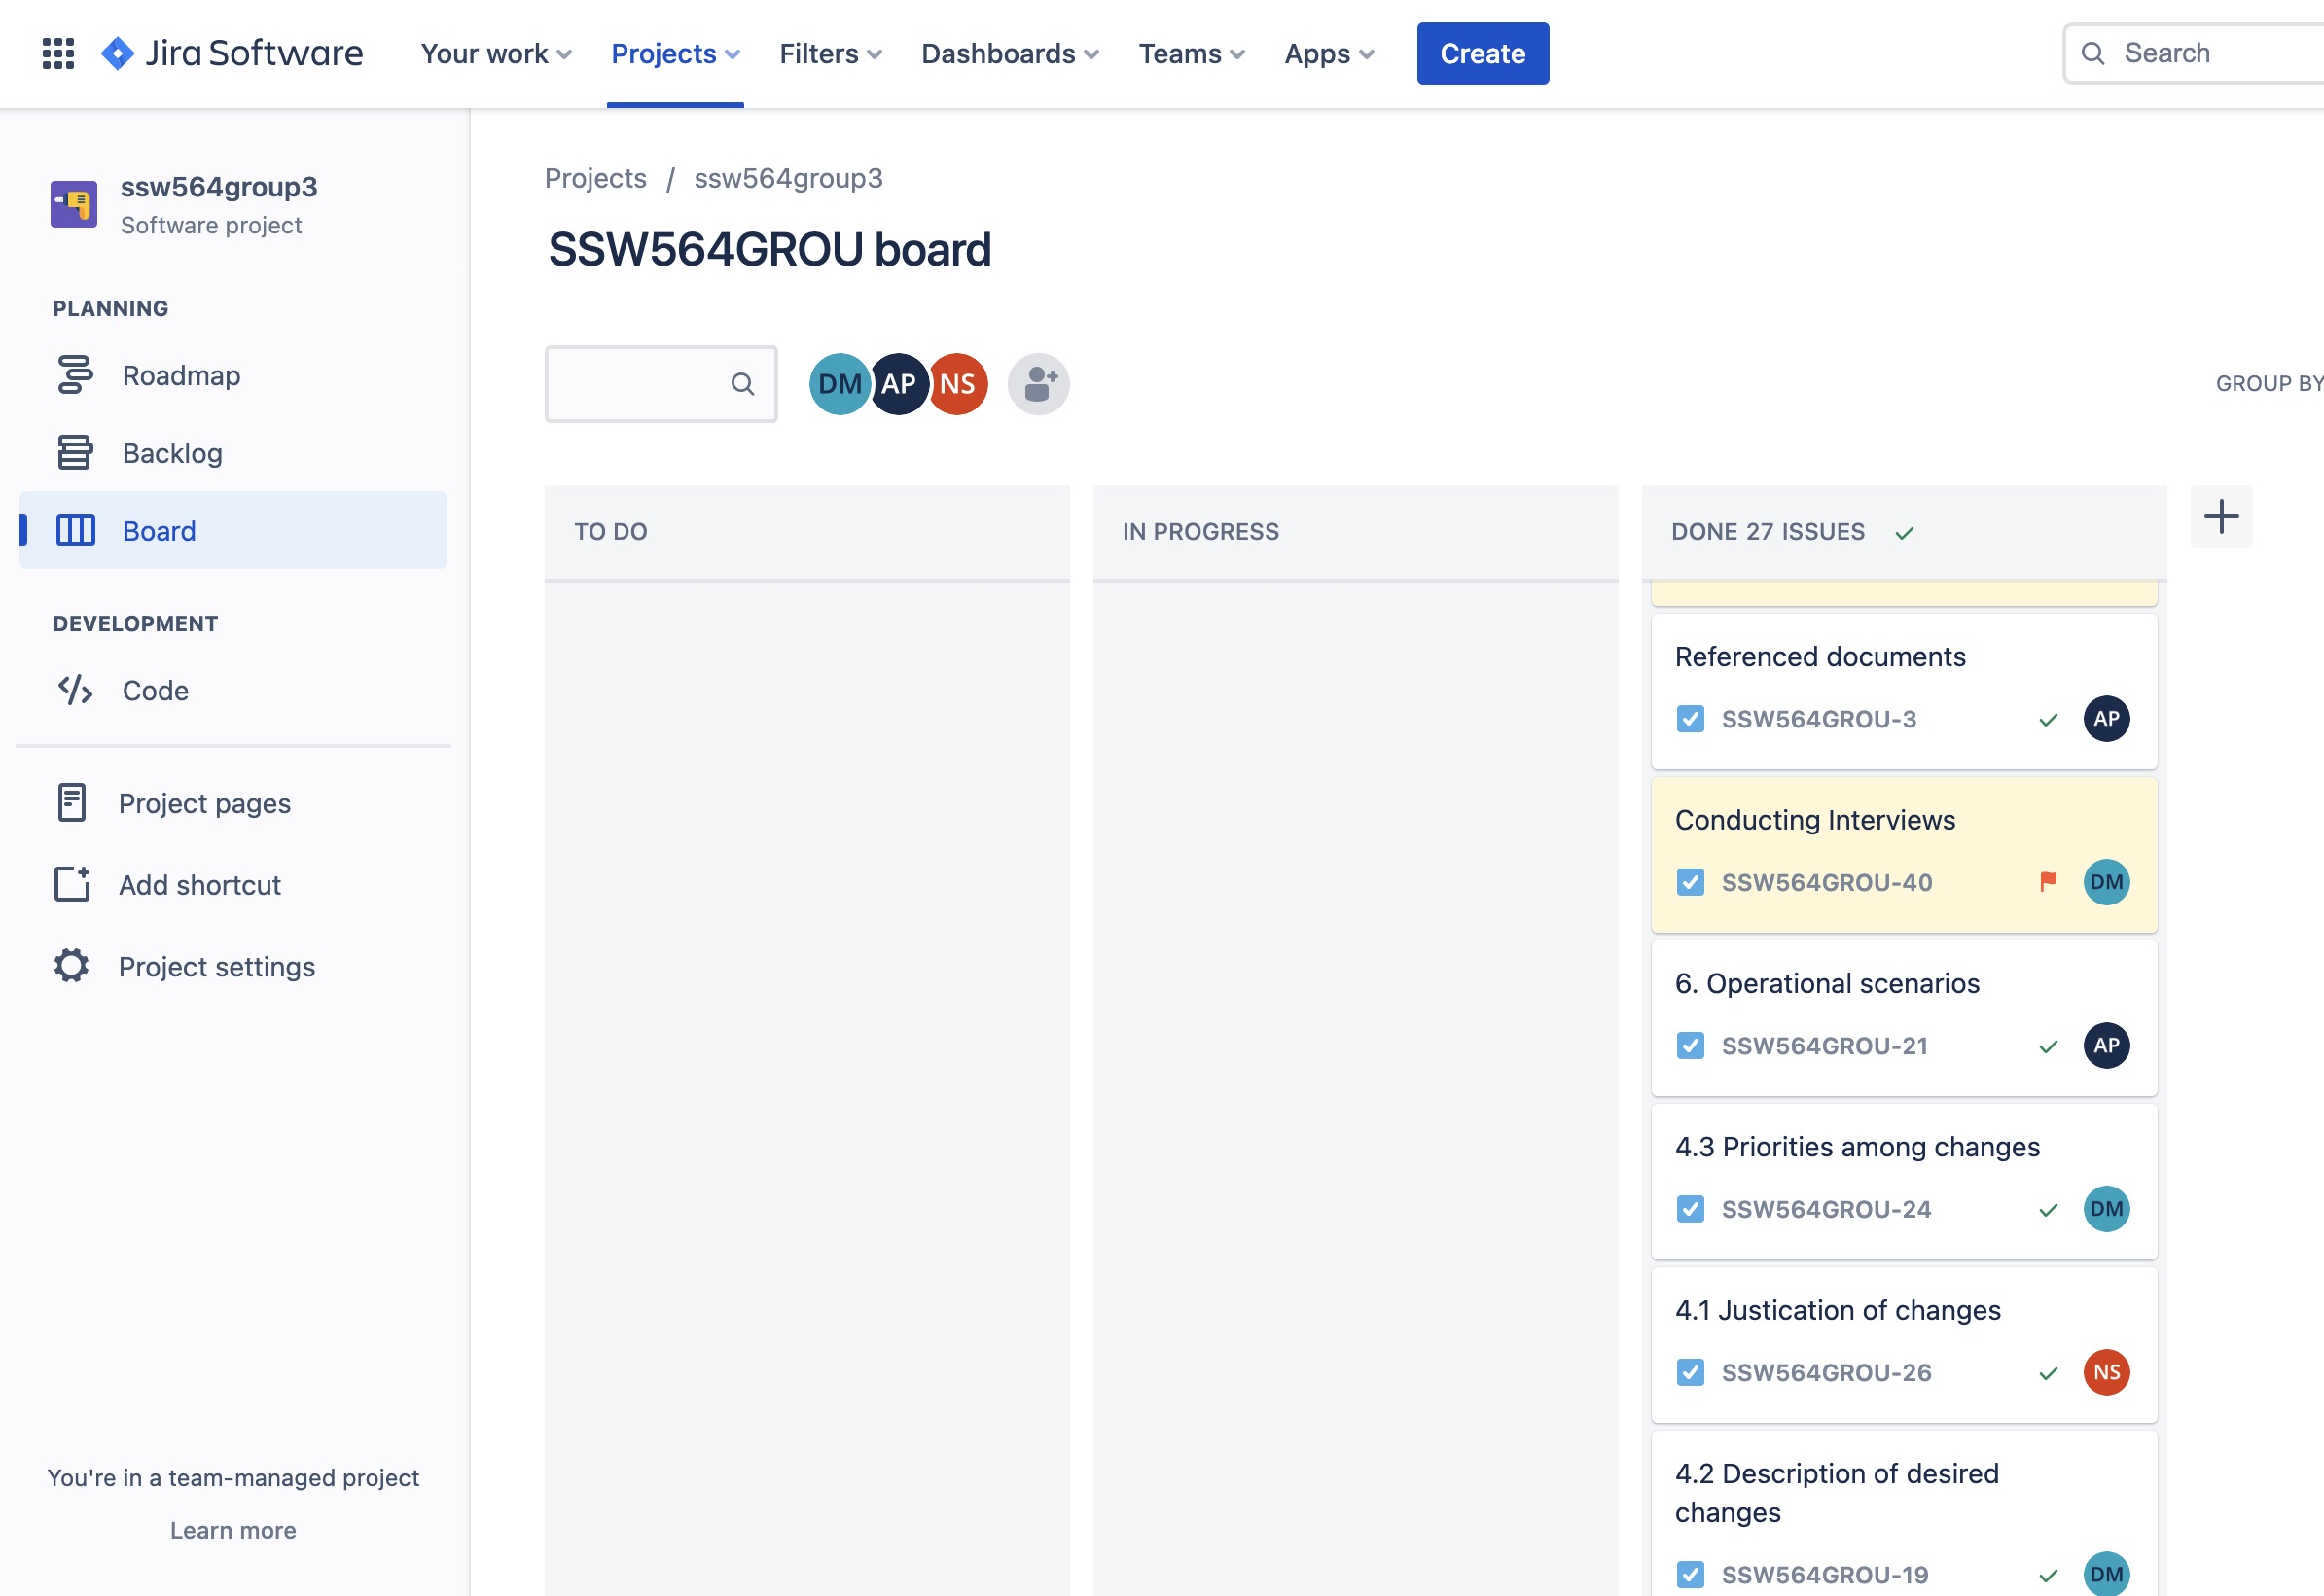
\includegraphics[width=9cm]{Figures/0DA589D3-1556-4FB9-9B0C-23CCDA029EBB_1_201_a.jpeg}
  \caption{Jira Homepage created for the project}
\label{}
\end{figure}
\newpage
\chapter{Analysis of the proposed system \\ 
% \small{\textit{-- Author Name}}
\index{Analysis of the proposed system}
\label{Chapter::Analysisoftheproposedsystem}}
\section{Summary of improvements \label{Section::Summaryofimprovements}}
\begin{enumerate}
    \item Multi-store support: The proposed system will allow for centralized inventory control across multiple locations, enabling inventory transfers between stores.

    \item Mobile access: The proposed system will provide mobile access, allowing for remote inventory management and reducing the need for physical presence in the store.

    \item Customizable alerts: The proposed system will enable customizable alerts to notify store managers and staff of low inventory levels, stockouts, and other inventory-related issues.

    \item Integration with POS system: The proposed system will integrate with the point-of-sale (POS) system, automatically updating inventory levels based on sales transactions, reducing errors related to manual data entry.

    \item Vendor management: The proposed system will include vendor management functionality, allowing for the optimization of the purchasing process and timely delivery of goods.
\end{enumerate}
\noindent
Overall, the proposed system will improve inventory accuracy, increase efficiency, and reduce costs, making it a worthwhile investment.

\section{Disadvantages and limitations \label{Section::Disadvantagesandlimitations}}
\begin{enumerate}


    \item Cost: Developing and implementing the proposed system will require a significant investment of time and resources, including software development, hardware procurement, and staff training.

    \item Technical challenges: The development and implementation of the proposed system may encounter technical challenges, including software bugs, hardware failures, or integration issues with other systems.

    \item Organizational change: The proposed system may require changes to existing workflows or data management practices, which may be disruptive and require staff training.

    \item Security concerns: Storing inventory data in a centralized system may pose security risks if not properly secured.
\end{enumerate}

\section{Alternatives and trade-offs considered \label{Section::Alternativesandtradeoffsconsidered}}
\begin{enumerate}
    \item Even though our system tries to fill in the gaps that are present in the market, the cost of doing that still remains unless and until the system scales and more retailers join, the cost of the system may remain high.
    \item To initially keep the system simple, we decided to keep english as the primary language used in the system. While, we have seen that many of the users may not be well versed with a particular language. However, this ensures a faster development of the initial product in english while later extending support to other languages.
    \item Targeted use of Cloud increases the maintenance and upfront cost of the system, however, in the long run it ensures that the system has higher availability and better scalability.
    \item Incorporation of the system may require changes to the existing workflow as in the initial software versions are designed with specific workflows in mind. Again to ensure a smoother initial release. This workflow is the one that we found to be the most commonly used.
    \item Incorporation of an advanced prediction system for forecasting inventory was considered but the resources required for it may make the system unfeasible. Thus, it should not be a part of the main system. 
\end{enumerate}
\newpage
\chapter{Notes \\ 
% \small{\textit{-- Author Name}}
\index{Notes}
\label{Chapter::Notes}}

\section{Project Mission Statement \label{Section::projectmissionstatement}}
\section{Key Stakeholders \label{Section::keystakeholders}}
\section{Key Drivers \label{Section::keydrivers}}
\section{Key Constraints \label{Section::keyconstraints}}
\section{Key Requirements \label{Section::keyrequirements}}
\section{Requirement Elicitation \label{Section::requirementelicitation}}
\section{Requirement Validation and Analysis \label{Section::requirementvalidationandanalysis}}
\section{Users \label{Section::users}}
\section{JIRA \label{Section::jira}}
\section{GitHub \label{Section::github}}
\begin{itemize}    
    \item The system does not take into account the any mishaps or exceptions in the process unless explicitly informed about it as no sensors are information collection systems are incorporated.
    \item The system may not be compliant to certain regional regulations and may need some customization for operations in such regions.
\end{itemize}

\bibliography{bibfile}
%\bibliographystyle{unsrt}
\bibliographystyle{IEEEtran}

%% Initial version by Darian Muresan, Ph.D.
% Edit and adjust as needed.

\documentclass[12pt]{cornell}

% add index support
\makeindex

% graphing programs
\usepackage{color}
\usepackage{psfrag}
\usepackage{verbatim}
\usepackage{fancyhdr}
%\usepackage{titlesec}
\usepackage{fancyvrb} 
% hyperlink programs
\usepackage[pdfmark, 
breaklinks=true, 
colorlinks=true,
citecolor=blue,
linkcolor=blue,
menucolor=black,
pagecolor=black,
urlcolor=blue
]{hyperref} % links in pdf
%\usepackage[colorlinks]{hyperref} % links in dvi
\usepackage{listings}
\usepackage{amsfonts} 
\usepackage{amssymb} 
%\usepackage{tabto}

\usepackage{tabularx,colortbl}
\usepackage[chapter]{algorithm} 
\usepackage{algorithmic} 
\usepackage{blindtext}
\usepackage{imakeidx}


\definecolor{DarkGreen}{rgb}{0,0.6,0}
\definecolor{mygreen}{rgb}{0,0.6,0}
\definecolor{mygray}{rgb}{0.5,0.5,0.5}
\definecolor{mymauve}{rgb}{0.58,0,0.82}

\usepackage{tocloft}
\usepackage{amsmath}
\usepackage{tcolorbox}
\usepackage{enumitem}
\usepackage{longtable}
%\usepackage{textcomp}
\usepackage{txfonts}

%part for \part titles
%chap for \chapter titles
%sec for \section titles
%subsec for \subsection titles
%subsubsec for \subsubsection titles
%para for \paragraph titles
%subpara for \subparagraph titles
%fig for figure \caption titles
%subfig for subfigure \caption titles
%tab for table \caption titles
%subtab for subtable \caption titles

% update chapter number spacing
\setlength{\cftchapnumwidth}{2em}
\setlength{\cftsecnumwidth}{2.5em}
\setlength{\cftsubsecnumwidth}{3.5em}
\setlength{\cftsubsubsecnumwidth}{4.5em}

\addtolength{\cftsecindent}{0.5em}
\addtolength{\cftsubsecindent}{0.5em}
\addtolength{\cftsubsubsecindent}{0.5em}

%\titlespacing*{\chapter}{0pt}{-50pt}{20pt}
%\titleformat{\chapter}[display]{\normalfont\huge\bfseries}{\chaptertitlename\ 
%\thechapter}{20pt}{\Huge}
%\pagestyle{fancy}
%\pagestyle{cornell}
%
%\rhead{F054-021-0172}
%\chead{Nonlinear Enhancement of Visual Target Detection (AF05-T021)}
%\lhead{GSTI}
%\lfoot{\scriptsize Use or disclosure of data on this page is subject
%to the restriction on the title page of this proposal.}
%\cfoot{}
%\rfoot{\thepage}

\newfont{\Bp}{msbm10}
\newfont{\BpBig}{msbm10 scaled\magstep2}
\newfont{\Sc}{eusm10}
\newfont{\ScBig}{eusm10 scaled\magstep3}
\newfont{\Fr}{eufm10}
\newfont{\FrBig}{eufm10 scaled\magstep1}

% some commands:
\newcommand{\dxi}{{\tt m\_xDeltaInput}}
\newcommand{\dyi}{{\tt m\_yDeltaInput}}
\newcommand{\dci}{{\tt m\_cDeltaInput}}
\newcommand{\dxo}{{\tt m\_xDeltaOutput}}
\newcommand{\dyo}{{\tt m\_yDeltaOutput}}
\newcommand{\dco}{{\tt m\_cDeltaOutput}}
\newcommand{\ttf}[1]{{\tt #1}}
\newcommand{\tbl}[2]{{\begin{tabular}{c} #1 \\ #2 \end{tabular}}}

\newcommand{\urltwo}[2]{\mbox{\href{#1}{\tt #2}}}
\newcommand{\qnorm}[1]{\|#1\|_{\bQ}}
\newcommand{\qdot}[2]{\lrb #1, #2 \rrb_{\bQ}}
\newcommand{\kdot}[2]{\lrb #1, #2 \rrb_{\bf k}}
\newcommand{\tdot}[2]{\lrb #1, #2 \rrb}
\newcommand{\mydiff}[2]{\lrb #1 - #2 \rrb}
\newcommand{\lena}{\textit{lena}}
\newcommand{\barb}{\textit{barbara}}
\newcommand{\boat}{\textit{boat}}
\newcommand{\leaves}{\textit{leaves}}
\newcommand{\rings}{\textit{rings}}
\newcommand{\treg}{\textit{train region}}
\newcommand{\dreg}{\textit{denoise region}}
\newcommand{\oreg}{\textit{overlap region}}
\newcommand{\sil}{\sigma_l^2}
\newcommand{\sn}{\sigma^2}
\newcommand{\bn}{{\mbox{\bf \FrBig N}}}
\newcommand{\n}{\mbox{\Fr N}}
%\newcommand{\bn}{\bf N}
%\newcommand{\n}{N}
\newcommand{\bY}{\textbf{Y}}
\newcommand{\bX}{\textbf{X}}
\newcommand{\bb}{\textbf{b}}
\newcommand{\bu}{\textbf{u}}
\newcommand{\bv}{\textbf{v}}
\newcommand{\by}{\textbf{y}}
\newcommand{\bx}{\textbf{x}}
\newcommand{\be}{\textbf{e}}
\newcommand{\bz}{\textbf{z}}
\newcommand{\bs}{\textbf{s}}
\newcommand{\bw}{\textbf{w}}
\newcommand{\bQ}{\textbf{Q}}
\newcommand{\bphi}{\textbf{$\phi$}}
\newcommand{\lsb}{\left[}
\newcommand{\rsb}{\right]}
\newcommand{\lrb}{\left(}
\newcommand{\rrb}{\right)}
\newcommand{\lcb}{\left\{}
\newcommand{\rcb}{\right\}}
\newcommand{\R}{\mbox{\BpBig R}}
\newcommand{\F}{{\cal F}}
\newcommand{\Fk}{\mbox{\Sc F}}
\newcommand{\bQF}{\textbf{Q}_{\mbox{\Sc F}}}
\newcommand{\N}{{\cal N}}
\newcommand{\xlz}{X_l(z)}
\newcommand{\xhz}{X_h(z)}
\newcommand{\xz}{X(z)}
\newcommand{\pr}{ perfect reconstruction }
\newcommand{\smb}{Smith-Barnwell }
\newcommand{\xw}{X(e^{j\omega})}
\newcommand{\xmw}{X(-e^{j\omega})}
\newcommand{\dw}{D(e^{j\omega})}
\newcommand{\dmw}{D(-e^{j\omega})}
\newcommand{\ew}{E(e^{j\omega})}
\newcommand{\emw}{E(-e^{j\omega})}
\newcommand{\fw}{F_0(e^{j\omega})}
\newcommand{\fmw}{F_0(-e^{j\omega})}
\newcommand{\hoz}{H_1(z)}
\newcommand{\hzz}{H_0(z)}
\newcommand{\goz}{G_1(z)}
\newcommand{\gzz}{G_0(z)}
\newcommand{\hzw}{H_{0}(e^{j\omega})}
\newcommand{\hzmw}{H_{0}(-e^{j\omega})}
\newcommand{\hzcw}{H_{0}(e^{-j\omega})}
\newcommand{\how}{H_1(e^{j\omega})}
\newcommand{\homw}{H_1(-e^{j\omega})}
\newcommand{\gzw}{G_0(e^{j\omega})}
\newcommand{\gzmw}{G_0(-e^{j\omega})}
\newcommand{\gow}{G_1(e^{j\omega})}
\newcommand{\gomw}{G_1(-e^{j\omega})}
\newcommand{\wl}{e^{-jwL}}
\newcommand{\aqua}{\textit{AQua with OR }}
\newtheorem{theorem}{Theorem}
\newtheorem{lemma}{Lemma}
\newtheorem{corollary}{Corollary}
\newtheorem{claim}{Claim}
\newtheorem{definition}{Definition}
\newenvironment{proof}{\noindent{\em Proof.}}{\ \hfill Q.E.D.}
%\newtheorem{moduleCount}{L}
\newcommand*{\labelfile}[1]{%
  \label{file:#1}%
}

\lstset{ %
  backgroundcolor=\color{white},   % choose the background color; you must add \usepackage{color} or \usepackage{xcolor}
  basicstyle=\footnotesize,        % the size of the fonts that are used for the code
  breakatwhitespace=false,         % sets if automatic breaks should only happen at whitespace
  breaklines=true,                 % sets automatic line breaking
  captionpos=b,                    % sets the caption-position to bottom
  commentstyle=\color{DarkGreen},    % comment style
  deletekeywords={...},            % if you want to delete keywords from the given language
  escapeinside={\%*}{*)},          % if you want to add LaTeX within your code
  extendedchars=true,              % lets you use non-ASCII characters; for 8-bits encodings only, does not work with UTF-8
  %frame=single,                   % adds a frame around the code
  keepspaces=true,                 % keeps spaces in text, useful for keeping indentation of code (possibly needs columns=flexible)
  keywordstyle=\color{blue},       % keyword style
  language=C++,                    % the language of the code
  morekeywords={*,...},            % if you want to add more keywords to the set
  numbers=left,                    % where to put the line-numbers; possible values are (none, left, right)
  numbersep=5pt,                   % how far the line-numbers are from the code
  numberstyle=\tiny\color{mygray}, % the style that is used for the line-numbers
  rulecolor=\color{black},         % if not set, the frame-color may be changed on line-breaks within not-black text (e.g. comments (green here))
  showspaces=false,                % show spaces everywhere adding particular underscores; it overrides 'showstringspaces'
  showstringspaces=false,          % underline spaces within strings only
  showtabs=false,                  % show tabs within strings adding particular underscores
  stepnumber=1,                    % the step between two line-numbers. If it's 1, each line will be numbered
  stringstyle=\color{mymauve}     % string literal style
  %tabsize=2,                      % sets default tabsize to 2 spaces
  %caption=\lstname                % show the filename of files included with \lstinputlisting; also try caption instead of title
}

% Uncomment draftcopy to get the word DRAFT boldly across the first page
%   By the way, xdvi won't show it but it will come out when you print
%\usepackage[light,all]{draftcopy}		% DRAFT on first page
%\draftcopySetGrey{.97}
%\draftcopyName{Confidential}{150}
%\draftcopFirstPage{1}

% Uncomment drafthead to get the date and DRAFT in the header of pages
% that are normallly numbered on the top, pages 2-n of each chapter for example
% This doesn't work with centered page numbers: \pagestyle{cornellc}
%\usepackage{drafthead}

% Including selective chapters:
% use this to selectively process chapters, etc.  Put a % in front of
% the sections that you don't want done this time.  Includes are
% used instead of \input so that LaTeX will keep track of chapters and
% pages without processing everything.  Don't let any spaces creep in
% around the words or it will not work!


\includeonly{
prologue,
manIntroduction,
Identifyprojecttitle,
Referenceddocuments,
Currentsystemorsituation,
Justificationforandnatureofchanges,
Conceptsfortheproposedsystem,
Operationalscenarios,
Summaryofimpacts,
Analysisoftheproposedsystem,
Notes

}

\makeindex

\begin{document}

\pagenumbering{roman}
\singlespacing
% File: prologue.tex
% Thesis prologue:  Title page, acknowledgements, table of contents,
% list of figures, and list of tables.
%
% this file is to be \include'd after the \begin{document}

% Cornell-style title page
\begin{titlepage}
        \title{Projects Assignments}
        \author{Ashay Pable\\Divyamshu Mandadi\\Neel Savani\\ Stevens.edu }
        \conferraldate{}{\today} \maketitle
\end{titlepage}

% Copyright page
%\begin{copyrightpage}
\makecopyright
%\end{copyrightpage}

% Abstract: the abstract body is pulled from the file abstract.tex;
%  the title is pulled from the \title command in the titlepage section
\begin{abstract}
        %\makeabstitle
        \input abstract      % puts the abstract file here
\end{abstract}

% Biographical information pulled from file bio.tex
%\begin{biosketch} \input bio \end{biosketch}

% Dedication (optional):  pulls information from file dedication.tex
%\begin{dedication} 
%\input dedicate 
%\end{dedication}

% Acknowledgements:  pulls information from file acknow
%\begin{acknowledgements} \input acknow \end{acknowledgements}

% Table of contents
\contentspage

% If you have no tables or figures put a % in front of the list page line
% List of tables
\tablelistpage

% List of figures
\figurelistpage



\setcounter{page}{1}        % set page counter
\pagenumbering{arabic}      % set page number style
\pagestyle{fancy}         % top right page numbers
%\pagestyle{cornell}
%\pagestyle{cornellc}       % centered page numbers, disables drafthead

\renewcommand{\chaptermark}[1]{\markboth{#1}{}}
\renewcommand{\sectionmark}[1]{\markright{#1}{}}

\fancyhead{} % clear all fields

\lhead{Chapter \thechapter}
%\lhead{\thechapter}
\chead{\leftmark}
\rhead{\thepage}


\lfoot{Chapter \thechapter}
\cfoot{\copyright Stevens -- \today \mbox{} -- Project Name}
\rfoot{\thepage}

\renewcommand{\headrulewidth}{0.4pt}
\renewcommand{\footrulewidth}{0.4pt}

%\rhead{F054-021-0172}
%\chead{Nonlinear Enhancement of Visual Target Detection (AF05-T021)}
%\lhead{GSTI}
%\lfoot{\scriptsize Use or disclosure of data on this page is subject
%to the restriction on the title page of this proposal.}
%\cfoot{}
%\rfoot{\thepage}


\singlespacing
% \chapter{Introduction \\
% \small{\textit{-- Author Name}} 
% % \index{Chapter!introduction}
% \index{introduction}
% \label{Chapter::Introduction}}

% \chapter{Analysis of the proposed system \\ 
% % \small{\textit{-- Author Name}}
% \index{Analysis of the proposed system}
% \label{Chapter::Analysisoftheproposedsystem}}

% % Add a section and label it so that we can reference it later
% \section{My Section \label{Section::MySection}}


% % add a new page
% \newpage

% Hi there world!  Here is an example of a note\footnote{Here is a reference 
% to Figure \ref{Figure::manAgile} and an indexed keyword\index{keyword}.}

\chapter{Identify project and Mission statement \\
% \small{\textit{-- Ashay Pable}} 
%\index{Chapter!Homework One -- Requirements}
\index{Identify project and Mission statement}
\label{Chapter::Identify project and Mission statement}}

% Add a section and label it so that we can reference it later
\section{Team Members \label{Section::teamMembers}}
\begin{enumerate}
  \item \textbf{Ashay Pable} : I am a Masters in Software Engineering student. I have worked as a software
developer for 4 years in India with a wide range of experience from Artificial Intelligence to
3D Graphics development. I have a keen interest in automation powered by AI and research
in contributing fields. My experience as a developer has made me realise the importance of
planning and documentation before initiation of a project
  \item \textbf{Divyamshu Mandadi} : My name is Divyamshu Mandadi and I’m currently in my third
semester doing my Masters in Software Engineering. Before moving to the US I have
worked as a Software Developer in India. My experience while working there combined
with the curiosity to learn more about the Software development processes led me here.
  \item \textbf{Neel Savani} : My name is Neel Savani. I had completed my under-graduation in Informa-
tion and Technology at birla vishwakarma mahavidhyalaya. I am currently in my second-
semester pursuing my masters in Software engineering. I am interested in developing soft-
ware.
\end{enumerate}

\section{Team Name \label{Section::teamName}}
"Group 3 - Inventory Management System for Retail Stores"
\section{Project Chosen \label{Section::projectChosen}}
\begin{itemize}
 \item Inventory Management system for Retail Stores.
 \item The project's goal is to create an intuitive and efficient inventory management system that will provide a retail business with real-time visibility into inventory levels and movement.
\end{itemize}
\section{Project Mission Statement \label{Section::projectMissionStatement}}
Our mission is to provide seamless and continuous supply of inventory so that customers needs are catered to in an efficient manner. Our system will provide an intuitive user interface that enables efficient recording and management of each item in the inventory. Retailers will be able to minimize stockouts, manage inventory levels for maximum profitability, and base data-driven choices on real-time inventory levels. This system provides a comprehensive solution that improves inventory management for retail establishments, frees up time, reduces expenses, and increases overall operational performance.

% \cite{GM1998}.

%\begin{figure}
%\centering
%\scalebox{0.8}{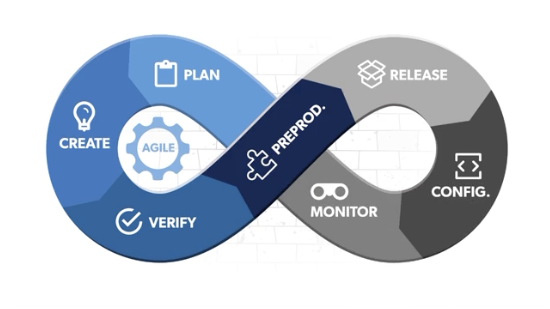
\includegraphics{Figures/manAgileProcess.png}}
%\caption{\label{Figure::manAgile} Figure of the continuous agile process.}
%\end{figure}

% add a new page
\newpage

\chapter{Referenced documents \\ 
% \small{\textit{-- Author Name}}
\index{Referenced documents}
\label{Chapter::Referenceddocuments}} 

Several recent studies, relevant research papers and articles with keywords such as “Inventory Management” and “Retail” or “Retail Sector” and “Operations Research” Databases such as Google Scholar, Science Direct and Z-library were also used. We also used Oracle Retail Store Inventory Management Documentation Library extensively to identify their features, limitations and how through our system we can mitigate them.\cite{ORACLE}

\newpage
\chapter{Current system or situation \\ 
% \small{\textit{-- Author Name}}
\index{Current system or situation}
\label{Chapter::Currentsystemorsituation}} 
\section{Background, objectives, and scope \label{Section::Backgroundobjectivesandscope}}
The instore inventory management system is an essential tool for managing inventory in a retail store. The system is responsible for tracking the movement of goods, monitoring stock levels, and ensuring that the right products are available at the right time. The current manual inventory management system is time-consuming, prone to errors, and lacks real-time visibility of inventory levels. The new instore inventory management system aims to address these challenges by automating the process, providing accurate and real-time inventory information, and enabling efficient and effective management of inventory levels.
The primary objective of the instore inventory management system is to improve the accuracy, efficiency, and effectiveness of inventory management in the retail store. Specifically, the system aims to achieve the following objectives:
\begin{enumerate}    
\item Real-time inventory visibility: Provide accurate and real-time visibility of inventory levels to store managers and staff.

\item Automated inventory tracking: Automate the process of tracking inventory movement, including receiving, stocking, and selling products.

\item Efficient inventory management: Enable efficient management of inventory levels, including setting reorder points, managing stock levels, and reducing waste.

\item Improved decision-making: Provide data analytics and reporting tools to support informed decision-making related to inventory management.
\end{enumerate}
The instore inventory management system will be designed to manage inventory for a single retail store. The system will be integrated with the existing point-of-sale (POS) system to provide real-time inventory information. The system will track the movement of goods from the time they are received into the store until they are sold or removed from inventory. The system will include features for setting reorder points, generating purchase orders, and monitoring stock levels. The system will also include reporting and data analytics tools to support informed decision-making related to inventory management.

The system will be designed to be user-friendly and intuitive to use, with minimal training required for store managers and staff. The system will be scalable, allowing for the addition of new products and the expansion of the store. The system will be designed to be compatible with existing hardware and software systems in the store. Finally, the system will be secure and reliable, ensuring the confidentiality and integrity of inventory data.

\section{Operational policies and constraints \label{Section::Operationalpoliciesandconstraints}}

\textbf{Operational policies:}
\begin{enumerate}
\item Access control: Access to the instore inventory management system will be restricted to authorized personnel only. Access credentials will be assigned on a need-to-know basis.
\item Data protection: The system will store inventory data in a secure and encrypted manner. Data backups will be taken regularly to ensure data integrity and availability in case of system failure.
\item Maintenance and support: The system will be maintained and supported by trained personnel to ensure optimal performance and reliability. Maintenance schedules will be developed to minimize disruptions to store operations.
\item Training and documentation: Store managers and staff will be provided with adequate training and documentation to ensure proper use of the system. Training will be ongoing, and documentation will be updated as needed.
\item Change management: Changes to the system, including upgrades and modifications, will be managed through a formal change management process. Changes will be tested and validated before implementation.

\end{enumerate}

\noindent
\textbf{Constraints:}
\begin{enumerate}
\item Budget: The implementation of the instore inventory management system will be subject to budgetary constraints. The cost of hardware, software, and personnel will need to be within the allocated budget.

\item Integration with existing systems: The system will need to be integrated with the existing point-of-sale (POS) system, which may have limitations on compatibility.

\item Technical limitations: The system will be subject to technical limitations, such as hardware capacity and bandwidth limitations.

\item User adoption: The success of the system will depend on the adoption by store managers and staff. The system will need to be user-friendly and intuitive to ensure adoption.

\item Regulatory compliance: The system will need to comply with all relevant regulatory requirements, including data privacy and security regulations.
\end{enumerate}

\section{Description of the current system or situation \label{Section::Descriptionofthecurrentsystemorsituation}}
The current inventory management system in the retail store is a manual process that is time-consuming and prone to errors. The process involves tracking inventory movement, monitoring stock levels, and placing orders for replenishment. The system relies on physical counts, spreadsheets, and manual record-keeping to track inventory.

The process begins with the receipt of goods from suppliers. The store manager or staff checks the goods against the purchase order and records the receipt in a manual log. The goods are then moved to the storage area, and the stock level is updated manually.

When items are sold, the store manager or staff records the sale in the point-of-sale (POS) system and manually updates the inventory count. When stock levels fall below a certain threshold, the store manager or staff manually creates a purchase order to replenish the inventory.

The current system has several limitations. Firstly, the manual process is time-consuming and prone to errors, leading to inaccurate inventory counts and stockouts. Secondly, the system lacks real-time visibility of inventory levels, making it challenging to manage stock levels effectively. Finally, the manual process does not provide data analytics and reporting tools to support informed decision-making related to inventory management.\cite{OR2020}
\begin{figure}[H]
  \centering
   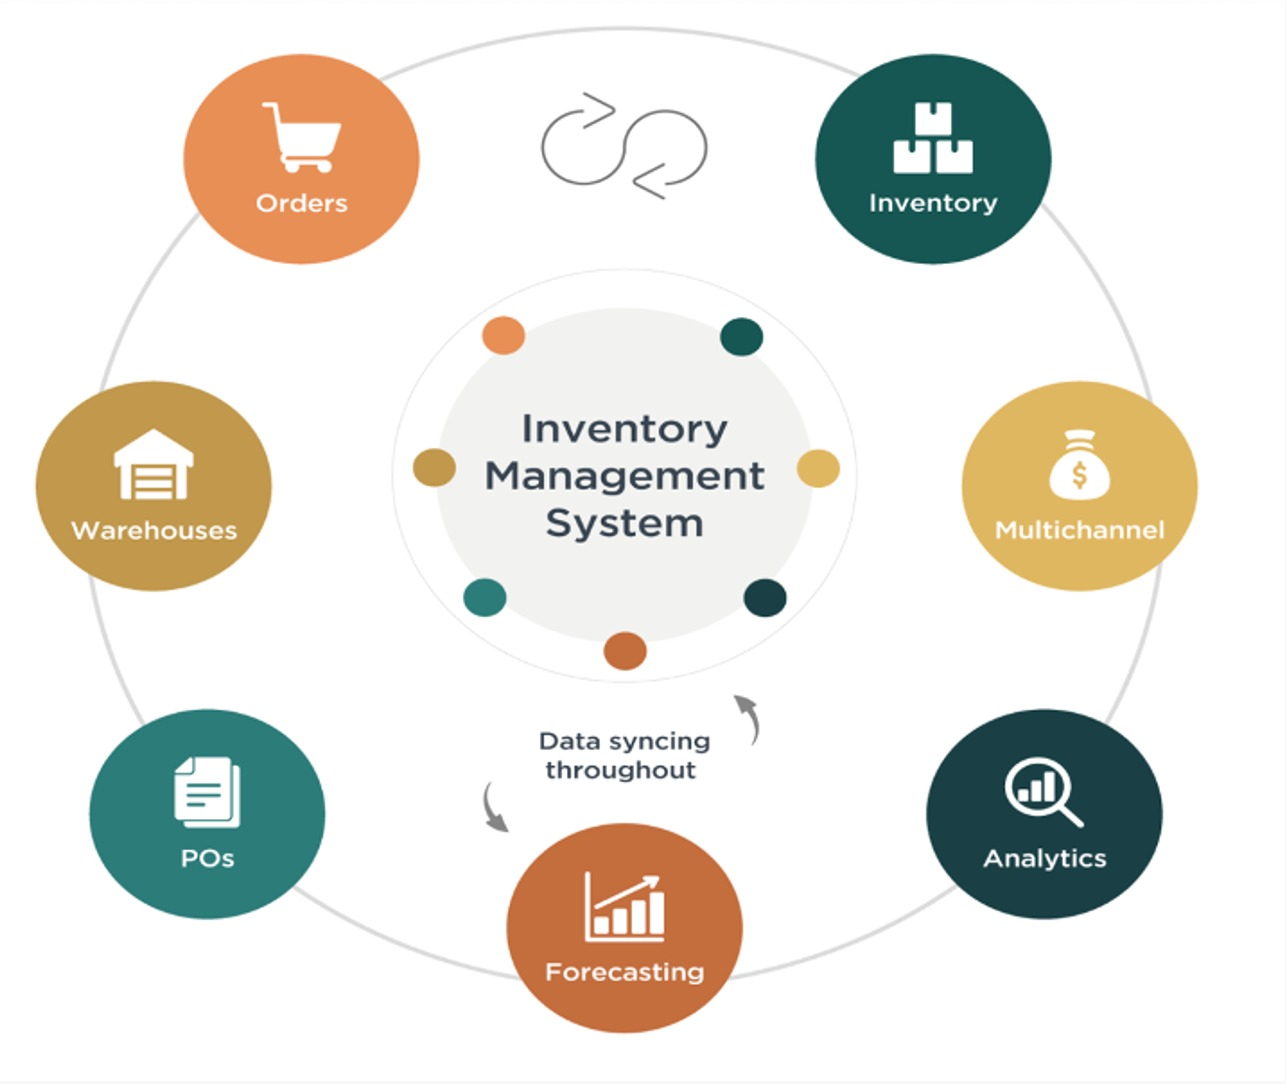
\includegraphics[width=9cm]{Figures/SpiritDiagram.jpeg}
  \caption{Overview Diagram}
\label{}
\end{figure}
\section{Modes of operation for the current system or situation \label{Section::Modesofoperationforthecurrentsystemorsituation}}
The current inventory management system in the retail store operates in the following modes:

\begin{enumerate}
    
\item Receiving mode: This mode is activated when goods are received from suppliers. The store manager or staff checks the goods against the purchase order and records the receipt in a manual log. The goods are then moved to the storage area, and the stock level is updated manually.

\item Stocking mode: This mode is activated when goods are moved from the storage area to the shelves or display areas. The store manager or staff manually updates the inventory count.

\item Selling mode: This mode is activated when items are sold to customers. The store manager or staff records the sale in the point-of-sale (POS) system and manually updates the inventory count.

\item Ordering mode: This mode is activated when stock levels fall below a certain threshold. The store manager or staff manually creates a purchase order to replenish the inventory.

\end{enumerate}

The current system operates in a sequential manner, with each mode depending on the previous mode's completion. The system lacks real-time visibility of inventory levels and does not provide automated inventory tracking or reporting tools.

\section{User classes and other involved personnel \label{Section::Userclassesandotherinvolvedpersonnel}}
The following are the user classes and other personnel involved in the instore inventory management system:

\begin{enumerate}

    \item Store manager: The store manager is responsible for managing the inventory and overseeing the instore inventory management system's operation. The store manager is responsible for setting up the system, assigning access credentials to authorized personnel, and ensuring the system's proper use.


    \item Store staff: The store staff is responsible for handling the goods, updating inventory levels, and generating reports using the instore inventory management system. The store staff will be provided with adequate training and documentation to ensure proper use of the system.

    \item IT personnel: The IT personnel will be responsible for    installing, configuring, and maintaining the hardware and software components of the system. They will also be responsible for ensuring the system's security, integrity, and availability.

    \item Suppliers: The suppliers will be involved in the system through the receipt of purchase orders generated by the system. The suppliers will need to ensure timely delivery of goods and accurate order fulfillment.

    \item Customers: The customers indirectly interact with the system by purchasing goods that are managed by the instore inventory management system. The system will ensure that the customers have access to the products they need when they need them, improving their shopping experience.
    
\end{enumerate}

The involvement of these user classes and personnel is critical to the success of the instore inventory management system, and their cooperation and support will be essential for the system's effective implementation and operation.

\section{Support environment \label{Section::Supportenvironment}}
\begin{enumerate}
    \item Help desk: A help desk will be set up to provide support and assistance to store managers and staff using the system. The help desk will be staffed by trained personnel who can provide technical assistance and troubleshooting support.

    \item Online documentation: The instore inventory management system will include online documentation that provides detailed instructions on how to use the system's features and functionality. The documentation will be regularly updated and available online for easy access.

    \item Training sessions: Store managers and staff will be provided with adequate training on the system's operation and functionality. Training sessions will be conducted both online and in-person and will be tailored to the specific needs of the user class.

    \item Maintenance and support team: A dedicated maintenance and support team will be responsible for ensuring the system's optimal performance and reliability. The team will be available to respond to system issues and perform maintenance tasks as required.

    \item Vendor support: The system vendor will provide technical support and assistance in case of system issues or malfunctions. The vendor will be responsible for ensuring that the system operates as intended and meets the user's requirements.
    
\end{enumerate}


\newpage
\chapter{Justification for and nature of changes \\ 
% \small{\textit{-- Author Name}}
\index{Justification for and nature of changes}
\label{Chapter::Justificationforandnatureofchanges}} 
\section{Justication of changes \label{Section::Justicationofchanges}}
The justification for these changes is to address several key issues identified through a recent analysis of our company's operations. This analysis revealed a number of inefficiencies and bottlenecks that have been negatively impacting productivity and profitability. The proposed changes aim to streamline workflows, improve communication and collaboration, and optimize resource allocation to achieve better results.

\noindent
There are several reasons why changes are required, including:

\begin{enumerate}

    \item New business requirements: The business requirements for the instore inventory management system may change as the business grows or as market conditions change. These changes may require modifications to the system to support new requirements.

    \item Technological advancements: Advancements in technology may provide new opportunities to improve the system's performance, reliability, and scalability. These advancements may require changes to the system to take advantage of the new capabilities.

    \item User feedback: Feedback from users may reveal areas where the system could be improved to better meet their needs. This feedback may prompt changes to the system's design or functionality.

    \item Regulatory requirements: Changes in regulatory requirements may require modifications to the system to ensure compliance with new regulations.

    \item External factors: External factors, such as changes in the competitive landscape or economic conditions, may require modifications to the system to remain competitive or to reduce costs.

\end{enumerate}

The nature of changes in the instore inventory management system can range from minor modifications to major overhauls. Changes may involve adding new functionality, modifying existing functionality, or removing functionality that is no longer required. Changes may also involve modifications to the system's architecture or infrastructure to improve performance, reliability, or scalability.


\section{Description of desired changes \label{Section::Descriptionofdesiredchanges}}
The instore inventory management system requires several changes to enhance its performance, reliability, and scalability. Some of the desired changes are:

\begin{enumerate}

    \item Multi-store support: The system will now support multiple stores, enabling store managers and staff to manage inventory across several locations. This change will provide centralized inventory control and enable inventory transfers between stores, reducing the risk of stockouts or overstocking.

    \item Mobile access: The system will now provide mobile access, allowing store managers and staff to access inventory data and perform inventory management tasks from anywhere at any time. This change will enable remote inventory management and reduce the need for physical presence in the store, increasing efficiency and reducing costs.

    \item Customizable alerts: The system will now enable customizable alerts that notify store managers and staff of low inventory levels, stockouts, and other inventory-related issues. These alerts can be customized to specific thresholds and sent via email, SMS, or in-app notifications. This change will help ensure timely inventory management and reduce the risk of stockouts or overstocking.

    \item Integration with POS system: The system will now integrate with the point-of-sale (POS) system, allowing inventory levels to be automatically updated based on sales transactions. This change will ensure accurate inventory tracking and reduce errors related to manual data entry.

    \item Vendor management: The system will now include vendor management functionality, enabling store managers and staff to manage vendor relationships and track vendor performance. This change will help optimize the purchasing process and ensure timely delivery of goods, reducing the risk of stockouts or overstocking.
    
\end{enumerate}
These changes will improve the system's functionality and make it more user-friendly, efficient, and accurate. The system will provide multi-store support, mobile access, customizable alerts, integration with the POS system, and vendor management functionality, enabling store managers and staff to manage inventory efficiently and effectively across multiple stores.

\section{Priorities among changes \label{Section::Prioritiesamongchanges}}
The priorities of the desired changes for the inventory management system would depend on the specific needs of the product. However, general benefits are:

\begin{enumerate}

    \item Integration with POS system: Integrating the inventory management system with the point-of-sale (POS) system should be a top priority as it would enable automatic inventory updates based on sales transactions. This would ensure accurate inventory tracking, reduce errors related to manual data entry, and provide real-time visibility into inventory levels.

    \item Customizable alerts: Implementing customizable alerts should be a high priority as it would notify store managers and staff of low inventory levels, stockouts, and other inventory-related issues, enabling timely inventory management and reducing the risk of stockouts or overstocking.

    \item Mobile access: Providing mobile access to the inventory management system should also be a high priority as it would enable store managers and staff to access inventory data and perform inventory management tasks from anywhere at any time, increasing efficiency and reducing costs.

    \item Vendor management: Including vendor management functionality should be a moderate priority as it would help optimize the purchasing process and ensure timely delivery of goods, reducing the risk of stockouts or overstocking.

    \item Multi-store support: Implementing multi-store support should be a moderate priority as it would enable store managers and staff to manage inventory across multiple locations, providing centralized inventory control and enabling inventory transfers between stores.

\end{enumerate}
Prioritizing these changes would enable the organization to implement the most critical improvements first and progressively enhance the system's functionality and efficiency over time.

\section{Changes considered but not included \label{Section::Changesconsideredbutnotincluded}}
During the development of the proposed instore inventory management system, several changes may have been considered but not included for various reasons. May be in a future iteration these can be incorporated. Some of these changes may include:

\begin{enumerate}
    \item RFID Technology: The use of RFID technology to track inventory in real-time is an option that may have been considered. However, this technology can be expensive to implement, and it may not be feasible for smaller organizations with limited resources.

    \item Advanced Artificial Intelligence: The use of artificial intelligence to automate inventory management tasks and make more accurate predictions have been considered. However, this technology can be complex and may require significant resources to implement and maintain. This will require a certain scale of operation before it may become profitable. Meanwhile, systems with lesser accuracy may suffice.

    \item Automatic Reorder: Automatic reorder functionality can be used to automatically generate purchase orders when inventory levels fall below a certain threshold. However, this feature involves a high risk factor and utilizing this without thorough testing and establishment may taint the products image in the market.

    \item Custom Barcode Generation: Barcode generation functionality can be used to generate barcodes for inventory items. However, This system may not be necessary as most products already come with a unique barcode. It is done only in case of threat with regards to barcode tampering, which only happens when the suppliers are non trusted entities, which is extremely rare.

\end{enumerate}

\newpage
\chapter{Concepts for the proposed system \\ 
% \small{\textit{-- Author Name}}
\index{Concepts for the proposed system}
\label{Chapter::Conceptsfortheproposedsystem}} 
\section{Background, objectives, and scope \label{Section::Backgroundobjectivesandscope}}
\begin{enumerate}
    
    \item Multi-store support: The system will support multiple stores, allowing store managers and staff to manage inventory across multiple locations. This will provide centralized inventory control and enable inventory transfers between stores.

    \item Mobile access: The system will provide mobile access, allowing store managers and staff to access inventory data and perform inventory management tasks from anywhere at any time. This will enable remote inventory management and reduce the need for physical presence in the store.

    \item Customizable alerts: The system will enable customizable alerts that notify store managers and staff of low inventory levels, stockouts, and other inventory-related issues. Alerts can be customized to specific thresholds and sent via email, SMS, or in-app notifications.

    \item Integration with POS system: The system will integrate with the point-of-sale (POS) system, allowing inventory levels to be automatically updated based on sales transactions. This will ensure accurate inventory tracking and reduce errors related to manual data entry.

    \item Vendor management: The system will include vendor management functionality, allowing store managers and staff to manage vendor relationships and track vendor performance. This will help optimize the purchasing process and ensure timely delivery of goods.

\end{enumerate}

\section{Operational policies and constraints \label{Section::Operationalpoliciesandconstraints}}
\textbf{Operational policies}:
\begin{enumerate}
    \item Access control: Access to the instore inventory management system will be restricted to authorized personnel only. Access credentials will be assigned on a need-to-know basis.

    \item Data protection: The system will store inventory data in a secure and encrypted manner. Data backups will be taken regularly to ensure data integrity and availability in case of system failure.

    \item Maintenance and support: The system will be maintained and supported by trained personnel to ensure optimal performance and reliability. Maintenance schedules will be developed to minimize disruptions to store operations.

    \item Training and documentation: Store managers and staff will be provided with adequate training and documentation to ensure proper use of the system. Training will be ongoing, and documentation will be updated as needed.

    \item Change management: Changes to the system, including upgrades and modifications, will be managed through a formal change management process. Changes will be tested and validated before implementation.
\end{enumerate}
\textbf{Constraints}:
\begin{enumerate}
    \item Budget: The implementation of the instore inventory management system will be subject to budgetary constraints. The cost of hardware, software, and personnel will need to be within the allocated budget.

    \item Integration with existing systems: The system will need to be integrated with the existing point-of-sale (POS) system, which may have limitations on compatibility.

    \item Technical limitations: The system will be subject to technical limitations, such as hardware availability and bandwidth limitations as the system may need to be operated in remote areas where connectivity is scarce.

    \item User adoption: The success of the system will depend on the adoption by store managers and staff. The system will need to be user-friendly and intuitive to ensure adoption.

    \item Regulatory compliance: The system will need to comply with all relevant regulatory requirements, including data privacy and security regulations.
\end{enumerate}
\section{Description of the proposed system \label{Section::Descriptionoftheproposedsystem}}

The proposed instore inventory management system is a web-based software solution designed to help retailers and store managers manage their inventory more efficiently and effectively. The system will include the following key features:

\begin{enumerate}
    \item Multi-store support: Supports multiple stores with centralized inventory control and transfers between stores.

    \item Mobile access: Provides mobile access for remote inventory management.

    \item Customizable alerts: Enables customizable alerts for low inventory levels and other inventory-related issues.

    \item Integration with POS system: Integrates with POS system for automatic inventory updates.

    \item Vendor management: Includes vendor management functionality for managing vendor relationships and tracking performance.

    \item Reporting and analytics: Provides real-time reporting and analytics for data-driven decision making.

    \item User roles and permissions: Has different user roles and permissions for authorized access and data security.

    \item Security and data privacy: Ensures security and privacy of inventory data and user information with robust security features.
\end{enumerate}
The proposed instore inventory management system will provide retailers and store managers with a comprehensive solution for managing their inventory more efficiently and effectively. It will enable centralized inventory control, remote inventory management, and real-time reporting and analytics to help optimize inventory management strategies and improve overall store performance.

\begin{figure}[H]
  \centering
   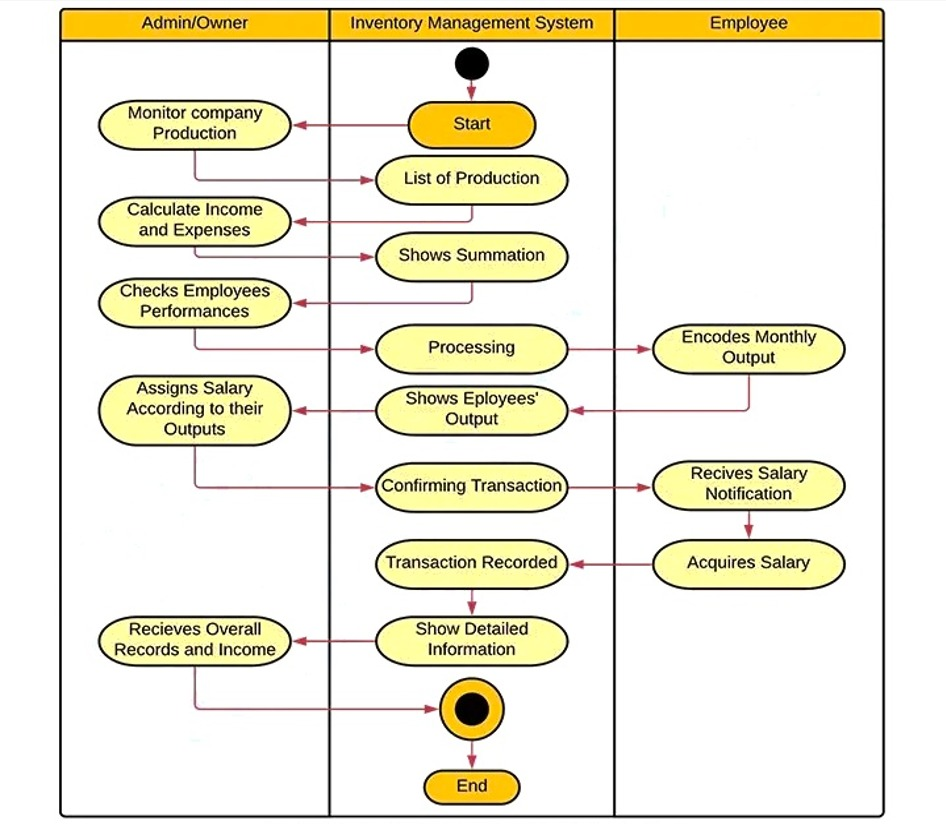
\includegraphics[width=9cm]{Figures/ActivityDiagram.jpeg}
  \caption{Activity Diagram of the system}
\label{}
\end{figure}

\begin{figure}[H]
  \centering
   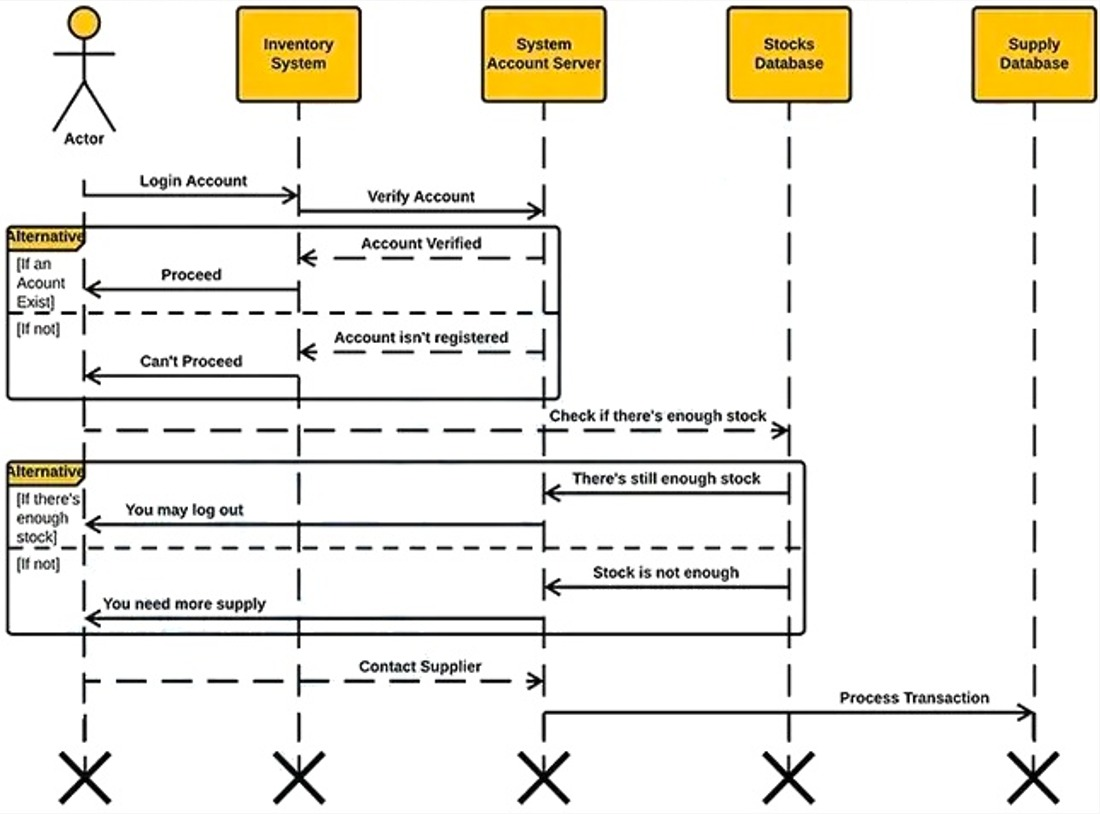
\includegraphics[width=9cm]{Figures/SequenceDiagram.jpeg}
  \caption{Sequence Diagram}
\label{}
\end{figure}

\section{Modes of operation \label{Section::Modesofoperation}}

\begin{enumerate}

    \item Online mode: Allows real-time access to inventory data through a web-based interface.

    \item Offline mode: Enables offline access to inventory data with local storage capabilities, and synchronization with the online system when an internet connection is available.

    \item Mobile mode: Provides mobile access to inventory data through a mobile application that is compatible with both Android and iOS devices.

    \item API mode: Allows integration with third-party systems through RESTful APIs for data sharing and system integration.

    \item Backup and recovery mode: Ensures data backup and recovery capabilities in case of system failures, data loss, or other disruptions.
\end{enumerate}

\section{User classes and other involved personnel \label{Section::Userclassesandotherinvolvedpersonnel}}
\begin{enumerate}
    \item Store managers: Responsible for managing inventory levels, overseeing stock movements, and making purchasing decisions.

    \item Sales staff: Responsible for tracking inventory movements, processing sales transactions, and updating inventory levels in real-time.

    \item Warehouse staff: Responsible for receiving and processing incoming shipments, managing inventory levels, and preparing outgoing shipments.

    \item IT staff: Responsible for system maintenance, upgrades, and technical support for the inventory management system.

    \item Auditors: Responsible for conducting periodic audits of inventory data and transactions to ensure accuracy and compliance with regulatory requirements.

    \item Vendors: Involved in the inventory management system as suppliers of goods and services, and can access the system for order management and delivery tracking.
\end{enumerate}
\begin{figure}[H]
  \centering
   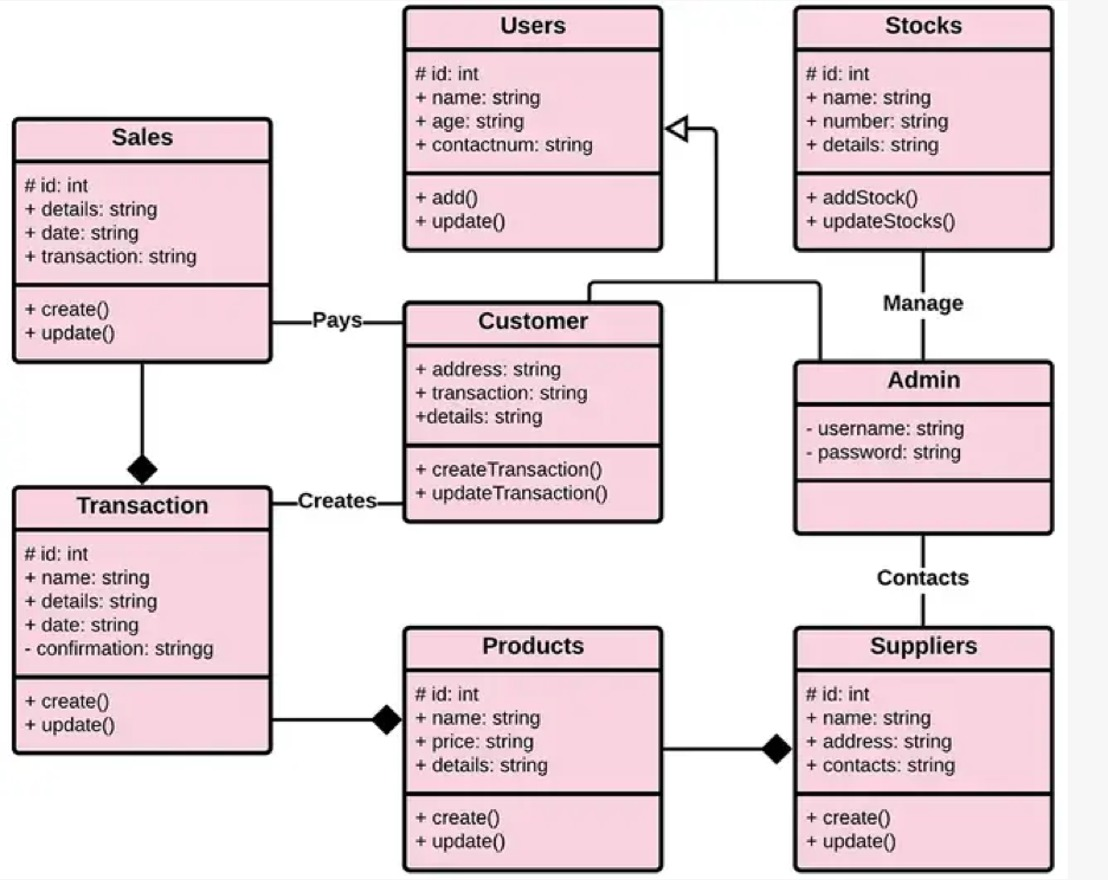
\includegraphics[width=9cm]{Figures/ClassDiagram.jpeg}
  \caption{Class Diagram of the proposed system}
\label{}
\end{figure}

\section{Support environment \label{Section::Supportenvironment}}

\begin{enumerate}
    \item Helpdesk and support services: A centralized helpdesk to provide technical support, assistance, and guidance to system users.

    \item Knowledge base and documentation: A comprehensive knowledge base and documentation system to provide users with resources and self-help tools to resolve issues and answer frequently asked questions.

    \item System maintenance and upgrades: Regular maintenance and upgrades of the system to ensure optimal performance, reliability, and security.

    \item Training and education: Training and education programs for users to ensure they have the necessary knowledge and skills to effectively use the system.

    \item User feedback and feature requests: A mechanism for users to provide feedback and suggest new features and enhancements to the system.
\end{enumerate}
\newpage
\chapter{Operational scenarios \\ 
% \small{\textit{-- Author Name}}
\index{Operational scenarios}
\label{Chapter::Operationalscenarios}} 
\begin{enumerate}
    \item Managing inventory across multiple stores: A store manager can log into the system and view inventory levels across multiple stores, transfer inventory between stores as needed, and receive alerts for low inventory levels or stockouts.


\begin{figure}[H]
  \centering
   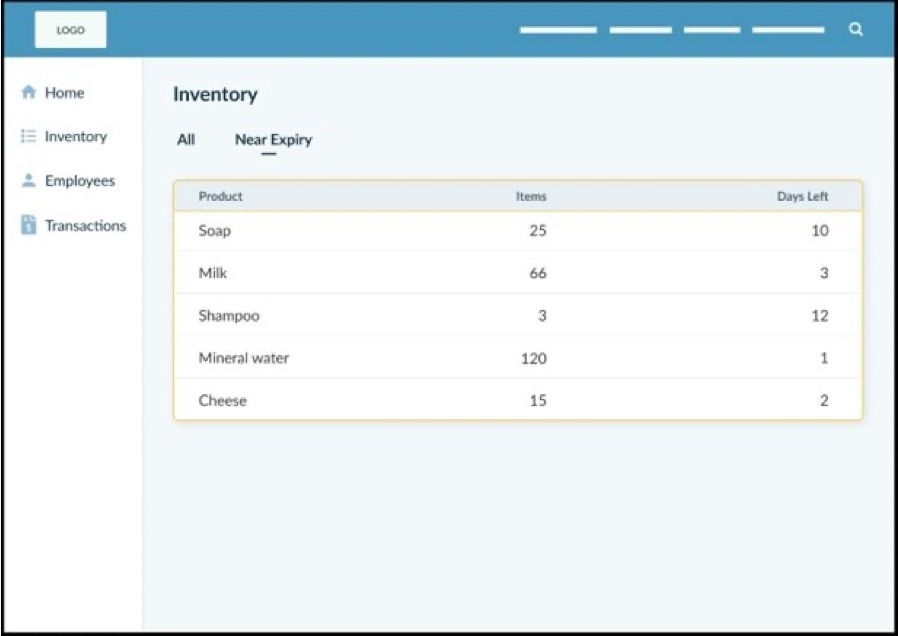
\includegraphics[width=9cm]{Figures/Figma2.jpeg}
  \caption{Inventory tab in the system}
\label{}
\end{figure}

    \item Mobile access for inventory management: A store employee can use the mobile app to access inventory data, update inventory levels, and perform inventory management tasks from anywhere, allowing for more flexibility in managing inventory.

    \begin{figure}[H]
  \centering
   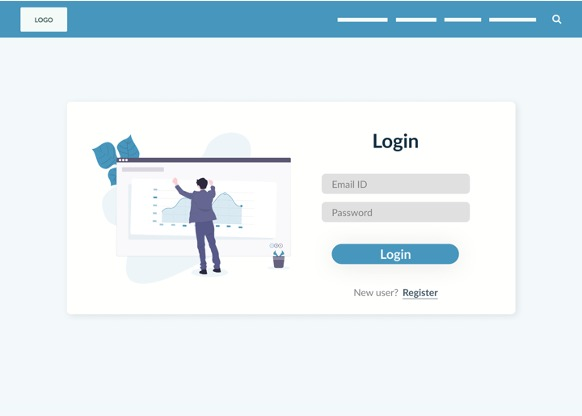
\includegraphics[width=9cm]{Figures/Figma4.jpeg}
  \caption{Login page}
\label{}
\end{figure}

\begin{figure}[H]
  \centering
   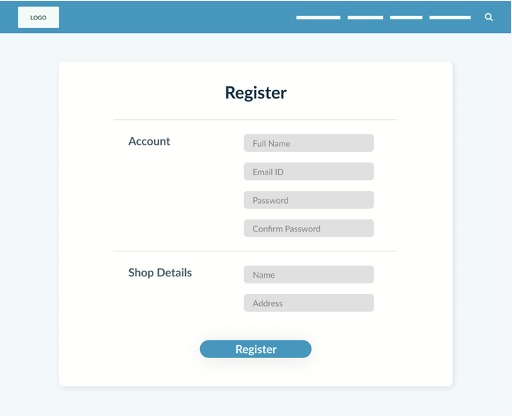
\includegraphics[width=9cm]{Figures/Figma3.jpeg}
  \caption{Registration Page}
\label{}
\end{figure}

\begin{figure}[H]
  \centering
   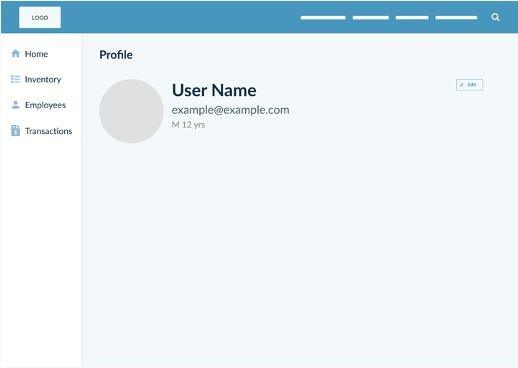
\includegraphics[width=9cm]{Figures/Figma6.jpeg}
  \caption{User profile}
\label{}
\end{figure}

    \item Customizable alerts for inventory issues: A store manager can set up customizable alerts for low inventory levels, stockouts, and other inventory-related issues, receiving notifications via email, SMS, or in-app notifications.

    
    \begin{figure}[H]
  \centering
   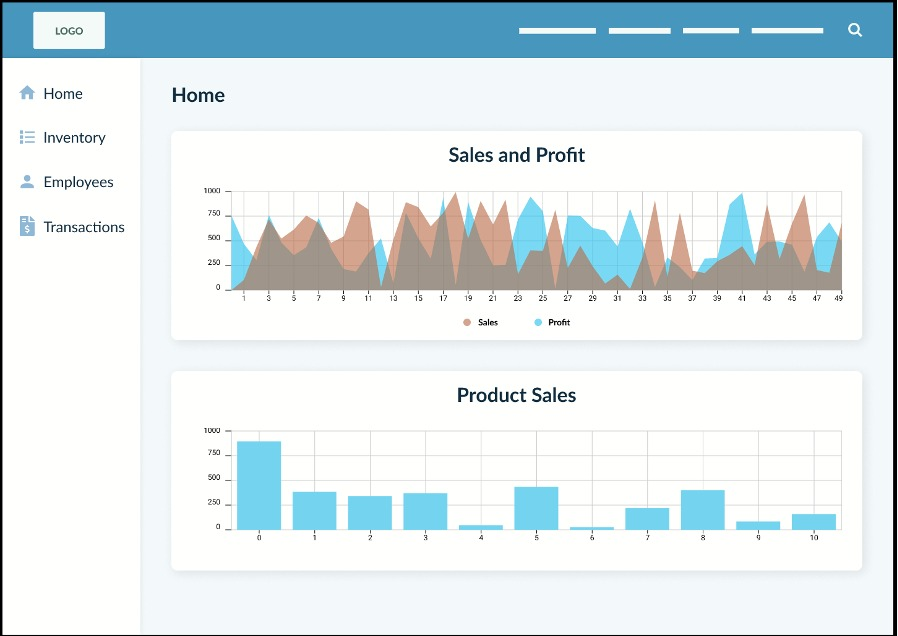
\includegraphics[width=9cm]{Figures/Figma1.jpeg}
  \caption{Homepage of the system}
\label{}
\end{figure}

    \item Automatic updates based on sales transactions: When a customer makes a purchase using the POS system, the inventory management system automatically updates inventory levels, ensuring accurate inventory tracking and reducing errors related to manual data entry.

    \begin{figure}[H]
  \centering
   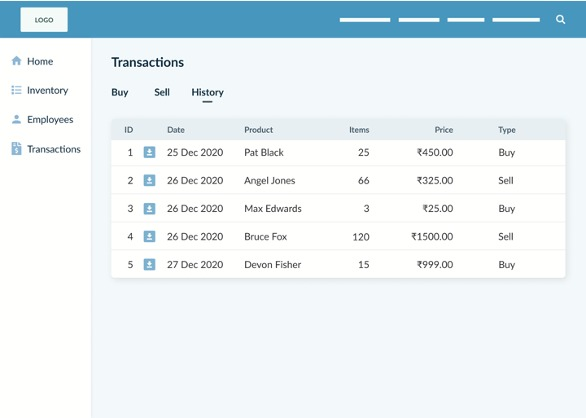
\includegraphics[width=9cm]{Figures/Figma7.jpeg}
  \caption{Transactions History tab}
\label{}
\end{figure}

\begin{figure}[H]
  \centering
   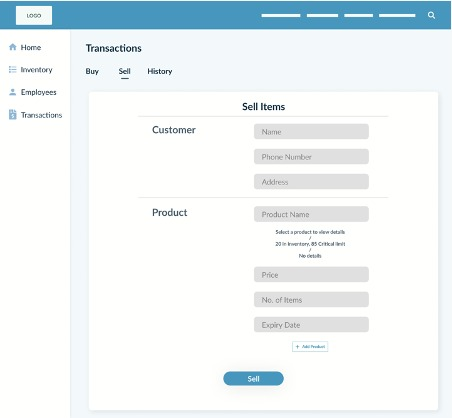
\includegraphics[width=9cm]{Figures/Figma8.jpeg}
  \caption{Transaction Details for selling items}
\label{}
\end{figure}

\begin{figure}[H]
  \centering
   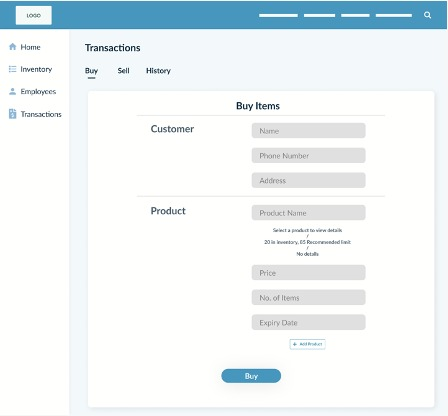
\includegraphics[width=9cm]{Figures/Figma5.jpeg}
  \caption{Transaction Details for buying items}
\label{}
\end{figure}

    \item Managing vendor relationships: A store manager can use the vendor management functionality to track vendor performance, manage purchase orders, and ensure timely delivery of goods, improving the efficiency of the purchasing process and reducing inventory-related issues.
\end{enumerate}
\newpage
\chapter{Summary of impacts \\ 
% \small{\textit{-- Author Name}}
\index{Summary of impacts}
\label{Chapter::Summaryofimpacts}} 
\section{Operational impacts \label{Section::Operationalimpacts}}
\begin{enumerate}
    \item Centralized inventory control: The ability to manage inventory across multiple stores in a centralized manner will lead to greater efficiency and accuracy in inventory tracking and management.

    \item Mobile access: The ability to access inventory data and perform inventory management tasks remotely will increase flexibility and enable more efficient use of staff time.

    \item Customizable alerts: The ability to receive alerts for low inventory levels, stockouts, and other inventory-related issues will improve inventory management and reduce the risk of stockouts and overstocking.

    \item Integration with POS system: The integration of the inventory management system with the point-of-sale system will ensure that inventory levels are automatically updated based on sales transactions, reducing errors and improving accuracy.

    \item Vendor management: The inclusion of vendor management functionality will streamline the purchasing process and improve vendor relationships, leading to more timely delivery of goods and better inventory management.
\end{enumerate}
\section{Organizational impacts \label{Section::Organizationalimpacts}}
\begin{enumerate}
    \item Improved inventory accuracy: The proposed system's automatic updates and centralized inventory control will improve inventory accuracy, reducing errors related to manual data entry and providing more accurate inventory data.

    \item Increased efficiency: Mobile access, customizable alerts, and vendor management functionality will increase the efficiency of inventory management tasks, allowing store managers and staff to manage inventory more quickly and easily.

    \item Reduced costs: Improved inventory accuracy and efficiency will reduce costs associated with overstocking, stockouts, and other inventory-related issues. Additionally, vendor management functionality can help optimize the purchasing process and reduce costs associated with late or incorrect deliveries.
\end{enumerate}

\section{Impacts during development \label{Section::Impactsduringdevelopment}}
\begin{enumerate}
    \item Time and resource requirements: Developing the proposed system will require a significant investment of time and resources, including software development, hardware procurement, and staff training.

    \item Potential disruptions to current operations: The development process may disrupt current inventory management processes, especially if the new system requires changes to existing workflows or data management practices.

    \item Collaboration and communication: Developing the proposed system will require collaboration and communication between developers, project managers, store managers, and other stakeholders to ensure that the system meets their needs and is properly integrated into their workflows.

    \item Technical challenges: The development process may encounter technical challenges, including software bugs, hardware failures, or integration issues with other systems.
\end{enumerate}

\noindent
The technical challenges can be tracked and planned around by utilizing a Bug reporting and job management software. We propose the use of JIRA.
\begin{figure}[H]
  \centering
   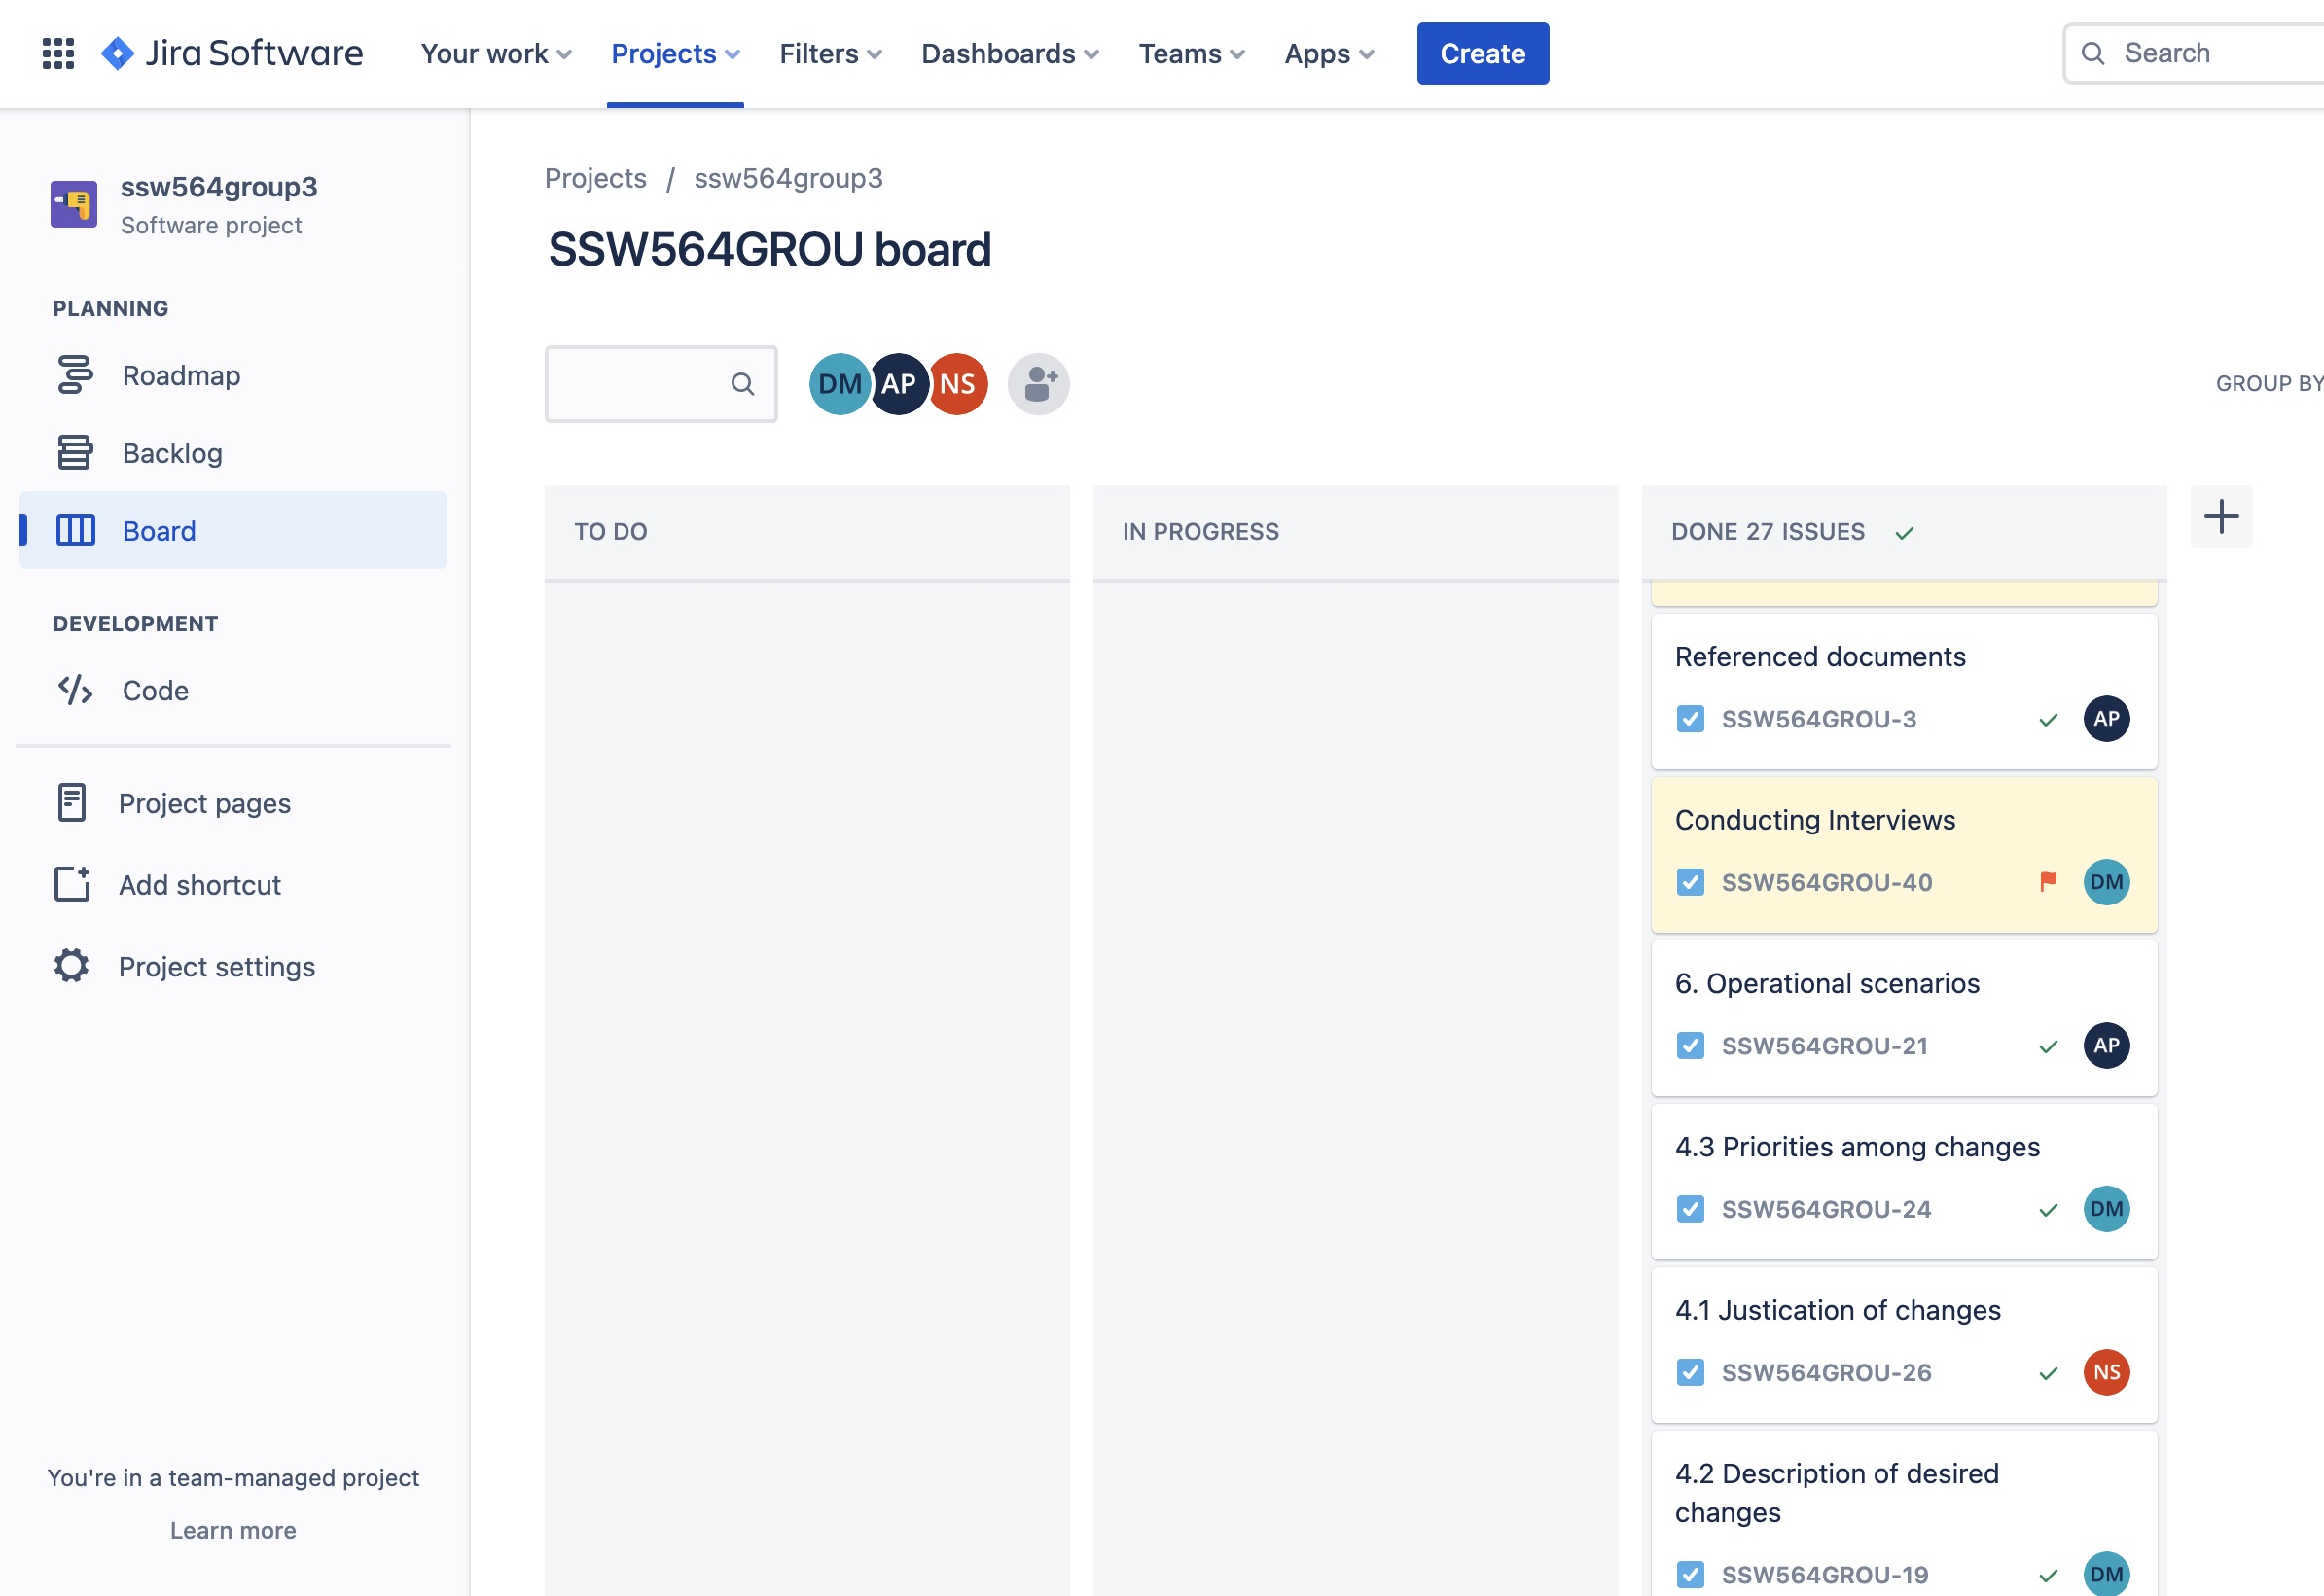
\includegraphics[width=9cm]{Figures/0DA589D3-1556-4FB9-9B0C-23CCDA029EBB_1_201_a.jpeg}
  \caption{Jira Homepage created for the project}
\label{}
\end{figure}
\newpage
\chapter{Analysis of the proposed system \\ 
% \small{\textit{-- Author Name}}
\index{Analysis of the proposed system}
\label{Chapter::Analysisoftheproposedsystem}}
\section{Summary of improvements \label{Section::Summaryofimprovements}}
\begin{enumerate}
    \item Multi-store support: The proposed system will allow for centralized inventory control across multiple locations, enabling inventory transfers between stores.

    \item Mobile access: The proposed system will provide mobile access, allowing for remote inventory management and reducing the need for physical presence in the store.

    \item Customizable alerts: The proposed system will enable customizable alerts to notify store managers and staff of low inventory levels, stockouts, and other inventory-related issues.

    \item Integration with POS system: The proposed system will integrate with the point-of-sale (POS) system, automatically updating inventory levels based on sales transactions, reducing errors related to manual data entry.

    \item Vendor management: The proposed system will include vendor management functionality, allowing for the optimization of the purchasing process and timely delivery of goods.
\end{enumerate}
\noindent
Overall, the proposed system will improve inventory accuracy, increase efficiency, and reduce costs, making it a worthwhile investment.

\section{Disadvantages and limitations \label{Section::Disadvantagesandlimitations}}
\begin{enumerate}


    \item Cost: Developing and implementing the proposed system will require a significant investment of time and resources, including software development, hardware procurement, and staff training.

    \item Technical challenges: The development and implementation of the proposed system may encounter technical challenges, including software bugs, hardware failures, or integration issues with other systems.

    \item Organizational change: The proposed system may require changes to existing workflows or data management practices, which may be disruptive and require staff training.

    \item Security concerns: Storing inventory data in a centralized system may pose security risks if not properly secured.
\end{enumerate}

\section{Alternatives and trade-offs considered \label{Section::Alternativesandtradeoffsconsidered}}
\begin{enumerate}
    \item Even though our system tries to fill in the gaps that are present in the market, the cost of doing that still remains unless and until the system scales and more retailers join, the cost of the system may remain high.
    \item To initially keep the system simple, we decided to keep english as the primary language used in the system. While, we have seen that many of the users may not be well versed with a particular language. However, this ensures a faster development of the initial product in english while later extending support to other languages.
    \item Targeted use of Cloud increases the maintenance and upfront cost of the system, however, in the long run it ensures that the system has higher availability and better scalability.
    \item Incorporation of the system may require changes to the existing workflow as in the initial software versions are designed with specific workflows in mind. Again to ensure a smoother initial release. This workflow is the one that we found to be the most commonly used.
    \item Incorporation of an advanced prediction system for forecasting inventory was considered but the resources required for it may make the system unfeasible. Thus, it should not be a part of the main system. 
\end{enumerate}
\newpage
\chapter{Notes \\ 
% \small{\textit{-- Author Name}}
\index{Notes}
\label{Chapter::Notes}}

\section{Project Mission Statement \label{Section::projectmissionstatement}}
\section{Key Stakeholders \label{Section::keystakeholders}}
\section{Key Drivers \label{Section::keydrivers}}
\section{Key Constraints \label{Section::keyconstraints}}
\section{Key Requirements \label{Section::keyrequirements}}
\section{Requirement Elicitation \label{Section::requirementelicitation}}
\section{Requirement Validation and Analysis \label{Section::requirementvalidationandanalysis}}
\section{Users \label{Section::users}}
\section{JIRA \label{Section::jira}}
\section{GitHub \label{Section::github}}
\begin{itemize}    
    \item The system does not take into account the any mishaps or exceptions in the process unless explicitly informed about it as no sensors are information collection systems are incorporated.
    \item The system may not be compliant to certain regional regulations and may need some customization for operations in such regions.
\end{itemize}

\bibliography{bibfile}
%\bibliographystyle{unsrt}
\bibliographystyle{IEEEtran}

%% Initial version by Darian Muresan, Ph.D.
% Edit and adjust as needed.

\documentclass[12pt]{cornell}

% add index support
\makeindex

% graphing programs
\usepackage{color}
\usepackage{psfrag}
\usepackage{verbatim}
\usepackage{fancyhdr}
%\usepackage{titlesec}
\usepackage{fancyvrb} 
% hyperlink programs
\usepackage[pdfmark, 
breaklinks=true, 
colorlinks=true,
citecolor=blue,
linkcolor=blue,
menucolor=black,
pagecolor=black,
urlcolor=blue
]{hyperref} % links in pdf
%\usepackage[colorlinks]{hyperref} % links in dvi
\usepackage{listings}
\usepackage{amsfonts} 
\usepackage{amssymb} 
%\usepackage{tabto}

\usepackage{tabularx,colortbl}
\usepackage[chapter]{algorithm} 
\usepackage{algorithmic} 
\usepackage{blindtext}
\usepackage{imakeidx}


\definecolor{DarkGreen}{rgb}{0,0.6,0}
\definecolor{mygreen}{rgb}{0,0.6,0}
\definecolor{mygray}{rgb}{0.5,0.5,0.5}
\definecolor{mymauve}{rgb}{0.58,0,0.82}

\usepackage{tocloft}
\usepackage{amsmath}
\usepackage{tcolorbox}
\usepackage{enumitem}
\usepackage{longtable}
%\usepackage{textcomp}
\usepackage{txfonts}

%part for \part titles
%chap for \chapter titles
%sec for \section titles
%subsec for \subsection titles
%subsubsec for \subsubsection titles
%para for \paragraph titles
%subpara for \subparagraph titles
%fig for figure \caption titles
%subfig for subfigure \caption titles
%tab for table \caption titles
%subtab for subtable \caption titles

% update chapter number spacing
\setlength{\cftchapnumwidth}{2em}
\setlength{\cftsecnumwidth}{2.5em}
\setlength{\cftsubsecnumwidth}{3.5em}
\setlength{\cftsubsubsecnumwidth}{4.5em}

\addtolength{\cftsecindent}{0.5em}
\addtolength{\cftsubsecindent}{0.5em}
\addtolength{\cftsubsubsecindent}{0.5em}

%\titlespacing*{\chapter}{0pt}{-50pt}{20pt}
%\titleformat{\chapter}[display]{\normalfont\huge\bfseries}{\chaptertitlename\ 
%\thechapter}{20pt}{\Huge}
%\pagestyle{fancy}
%\pagestyle{cornell}
%
%\rhead{F054-021-0172}
%\chead{Nonlinear Enhancement of Visual Target Detection (AF05-T021)}
%\lhead{GSTI}
%\lfoot{\scriptsize Use or disclosure of data on this page is subject
%to the restriction on the title page of this proposal.}
%\cfoot{}
%\rfoot{\thepage}

\newfont{\Bp}{msbm10}
\newfont{\BpBig}{msbm10 scaled\magstep2}
\newfont{\Sc}{eusm10}
\newfont{\ScBig}{eusm10 scaled\magstep3}
\newfont{\Fr}{eufm10}
\newfont{\FrBig}{eufm10 scaled\magstep1}

% some commands:
\newcommand{\dxi}{{\tt m\_xDeltaInput}}
\newcommand{\dyi}{{\tt m\_yDeltaInput}}
\newcommand{\dci}{{\tt m\_cDeltaInput}}
\newcommand{\dxo}{{\tt m\_xDeltaOutput}}
\newcommand{\dyo}{{\tt m\_yDeltaOutput}}
\newcommand{\dco}{{\tt m\_cDeltaOutput}}
\newcommand{\ttf}[1]{{\tt #1}}
\newcommand{\tbl}[2]{{\begin{tabular}{c} #1 \\ #2 \end{tabular}}}

\newcommand{\urltwo}[2]{\mbox{\href{#1}{\tt #2}}}
\newcommand{\qnorm}[1]{\|#1\|_{\bQ}}
\newcommand{\qdot}[2]{\lrb #1, #2 \rrb_{\bQ}}
\newcommand{\kdot}[2]{\lrb #1, #2 \rrb_{\bf k}}
\newcommand{\tdot}[2]{\lrb #1, #2 \rrb}
\newcommand{\mydiff}[2]{\lrb #1 - #2 \rrb}
\newcommand{\lena}{\textit{lena}}
\newcommand{\barb}{\textit{barbara}}
\newcommand{\boat}{\textit{boat}}
\newcommand{\leaves}{\textit{leaves}}
\newcommand{\rings}{\textit{rings}}
\newcommand{\treg}{\textit{train region}}
\newcommand{\dreg}{\textit{denoise region}}
\newcommand{\oreg}{\textit{overlap region}}
\newcommand{\sil}{\sigma_l^2}
\newcommand{\sn}{\sigma^2}
\newcommand{\bn}{{\mbox{\bf \FrBig N}}}
\newcommand{\n}{\mbox{\Fr N}}
%\newcommand{\bn}{\bf N}
%\newcommand{\n}{N}
\newcommand{\bY}{\textbf{Y}}
\newcommand{\bX}{\textbf{X}}
\newcommand{\bb}{\textbf{b}}
\newcommand{\bu}{\textbf{u}}
\newcommand{\bv}{\textbf{v}}
\newcommand{\by}{\textbf{y}}
\newcommand{\bx}{\textbf{x}}
\newcommand{\be}{\textbf{e}}
\newcommand{\bz}{\textbf{z}}
\newcommand{\bs}{\textbf{s}}
\newcommand{\bw}{\textbf{w}}
\newcommand{\bQ}{\textbf{Q}}
\newcommand{\bphi}{\textbf{$\phi$}}
\newcommand{\lsb}{\left[}
\newcommand{\rsb}{\right]}
\newcommand{\lrb}{\left(}
\newcommand{\rrb}{\right)}
\newcommand{\lcb}{\left\{}
\newcommand{\rcb}{\right\}}
\newcommand{\R}{\mbox{\BpBig R}}
\newcommand{\F}{{\cal F}}
\newcommand{\Fk}{\mbox{\Sc F}}
\newcommand{\bQF}{\textbf{Q}_{\mbox{\Sc F}}}
\newcommand{\N}{{\cal N}}
\newcommand{\xlz}{X_l(z)}
\newcommand{\xhz}{X_h(z)}
\newcommand{\xz}{X(z)}
\newcommand{\pr}{ perfect reconstruction }
\newcommand{\smb}{Smith-Barnwell }
\newcommand{\xw}{X(e^{j\omega})}
\newcommand{\xmw}{X(-e^{j\omega})}
\newcommand{\dw}{D(e^{j\omega})}
\newcommand{\dmw}{D(-e^{j\omega})}
\newcommand{\ew}{E(e^{j\omega})}
\newcommand{\emw}{E(-e^{j\omega})}
\newcommand{\fw}{F_0(e^{j\omega})}
\newcommand{\fmw}{F_0(-e^{j\omega})}
\newcommand{\hoz}{H_1(z)}
\newcommand{\hzz}{H_0(z)}
\newcommand{\goz}{G_1(z)}
\newcommand{\gzz}{G_0(z)}
\newcommand{\hzw}{H_{0}(e^{j\omega})}
\newcommand{\hzmw}{H_{0}(-e^{j\omega})}
\newcommand{\hzcw}{H_{0}(e^{-j\omega})}
\newcommand{\how}{H_1(e^{j\omega})}
\newcommand{\homw}{H_1(-e^{j\omega})}
\newcommand{\gzw}{G_0(e^{j\omega})}
\newcommand{\gzmw}{G_0(-e^{j\omega})}
\newcommand{\gow}{G_1(e^{j\omega})}
\newcommand{\gomw}{G_1(-e^{j\omega})}
\newcommand{\wl}{e^{-jwL}}
\newcommand{\aqua}{\textit{AQua with OR }}
\newtheorem{theorem}{Theorem}
\newtheorem{lemma}{Lemma}
\newtheorem{corollary}{Corollary}
\newtheorem{claim}{Claim}
\newtheorem{definition}{Definition}
\newenvironment{proof}{\noindent{\em Proof.}}{\ \hfill Q.E.D.}
%\newtheorem{moduleCount}{L}
\newcommand*{\labelfile}[1]{%
  \label{file:#1}%
}

\lstset{ %
  backgroundcolor=\color{white},   % choose the background color; you must add \usepackage{color} or \usepackage{xcolor}
  basicstyle=\footnotesize,        % the size of the fonts that are used for the code
  breakatwhitespace=false,         % sets if automatic breaks should only happen at whitespace
  breaklines=true,                 % sets automatic line breaking
  captionpos=b,                    % sets the caption-position to bottom
  commentstyle=\color{DarkGreen},    % comment style
  deletekeywords={...},            % if you want to delete keywords from the given language
  escapeinside={\%*}{*)},          % if you want to add LaTeX within your code
  extendedchars=true,              % lets you use non-ASCII characters; for 8-bits encodings only, does not work with UTF-8
  %frame=single,                   % adds a frame around the code
  keepspaces=true,                 % keeps spaces in text, useful for keeping indentation of code (possibly needs columns=flexible)
  keywordstyle=\color{blue},       % keyword style
  language=C++,                    % the language of the code
  morekeywords={*,...},            % if you want to add more keywords to the set
  numbers=left,                    % where to put the line-numbers; possible values are (none, left, right)
  numbersep=5pt,                   % how far the line-numbers are from the code
  numberstyle=\tiny\color{mygray}, % the style that is used for the line-numbers
  rulecolor=\color{black},         % if not set, the frame-color may be changed on line-breaks within not-black text (e.g. comments (green here))
  showspaces=false,                % show spaces everywhere adding particular underscores; it overrides 'showstringspaces'
  showstringspaces=false,          % underline spaces within strings only
  showtabs=false,                  % show tabs within strings adding particular underscores
  stepnumber=1,                    % the step between two line-numbers. If it's 1, each line will be numbered
  stringstyle=\color{mymauve}     % string literal style
  %tabsize=2,                      % sets default tabsize to 2 spaces
  %caption=\lstname                % show the filename of files included with \lstinputlisting; also try caption instead of title
}

% Uncomment draftcopy to get the word DRAFT boldly across the first page
%   By the way, xdvi won't show it but it will come out when you print
%\usepackage[light,all]{draftcopy}		% DRAFT on first page
%\draftcopySetGrey{.97}
%\draftcopyName{Confidential}{150}
%\draftcopFirstPage{1}

% Uncomment drafthead to get the date and DRAFT in the header of pages
% that are normallly numbered on the top, pages 2-n of each chapter for example
% This doesn't work with centered page numbers: \pagestyle{cornellc}
%\usepackage{drafthead}

% Including selective chapters:
% use this to selectively process chapters, etc.  Put a % in front of
% the sections that you don't want done this time.  Includes are
% used instead of \input so that LaTeX will keep track of chapters and
% pages without processing everything.  Don't let any spaces creep in
% around the words or it will not work!


\includeonly{
prologue,
manIntroduction,
Identifyprojecttitle,
Referenceddocuments,
Currentsystemorsituation,
Justificationforandnatureofchanges,
Conceptsfortheproposedsystem,
Operationalscenarios,
Summaryofimpacts,
Analysisoftheproposedsystem,
Notes

}

\makeindex

\begin{document}

\pagenumbering{roman}
\singlespacing
\include{prologue}

\setcounter{page}{1}        % set page counter
\pagenumbering{arabic}      % set page number style
\pagestyle{fancy}         % top right page numbers
%\pagestyle{cornell}
%\pagestyle{cornellc}       % centered page numbers, disables drafthead

\renewcommand{\chaptermark}[1]{\markboth{#1}{}}
\renewcommand{\sectionmark}[1]{\markright{#1}{}}

\fancyhead{} % clear all fields

\lhead{Chapter \thechapter}
%\lhead{\thechapter}
\chead{\leftmark}
\rhead{\thepage}


\lfoot{Chapter \thechapter}
\cfoot{\copyright Stevens -- \today \mbox{} -- Project Name}
\rfoot{\thepage}

\renewcommand{\headrulewidth}{0.4pt}
\renewcommand{\footrulewidth}{0.4pt}

%\rhead{F054-021-0172}
%\chead{Nonlinear Enhancement of Visual Target Detection (AF05-T021)}
%\lhead{GSTI}
%\lfoot{\scriptsize Use or disclosure of data on this page is subject
%to the restriction on the title page of this proposal.}
%\cfoot{}
%\rfoot{\thepage}


\singlespacing
\include{manIntroduction}
\include{Identifyprojecttitle}
\include{Chapters/manReferenceddocuments}
\include{Chapters/manCurrentsystemorsituation}
\include{Chapters/manJustificationforandnatureofchanges}
\include{Chapters/manConceptsfortheproposedsystem}
\include{Chapters/manOperationalscenarios}
\include{Chapters/manSummaryofimpacts}
\include{Chapters/manAnalysisoftheproposedsystem}
\include{Chapters/manNotes}

\bibliography{bibfile}
%\bibliographystyle{unsrt}
\bibliographystyle{IEEEtran}

%\input{manual.ind}
\printindex
\end{document}

\printindex
\end{document}

\printindex
\end{document}

\printindex
\end{document}
